\documentclass[acmsmall,review,screen,nonacm]{acmart}

% Preserve the repository's single-column ACM review layout.
% TODO: Replace author metadata and add venue metadata and CCS concepts.
\usepackage{amsmath,booktabs,tabularx,array}
\usepackage{listings}
\usepackage{placeins}
\usepackage{float}
\usepackage{wrapstuff}
\usepackage{microtype}
\setcounter{secnumdepth}{3}
\setcounter{tocdepth}{3}
\lstdefinelanguage{TEPL}{
  morekeywords={dialect,op,attrs,axis,extent,coordinate,axes,semantics,dtype,bind,yield,let,rule,where,derive,from,import,as,use,auto,tensor},
  sensitive=true,morecomment=[l]{//},morestring=[b]"
}
\lstset{basicstyle=\normalfont\ttfamily\small,keywordstyle=\bfseries,
  commentstyle=\normalfont\ttfamily\color{black!60},
  columns=fullflexible,keepspaces=true,showstringspaces=false,
  breaklines=true,breakatwhitespace=true,frame=single,
  framerule=0.3pt,rulecolor=\color{black!25},xleftmargin=4pt,xrightmargin=4pt,
  captionpos=b}
\newcommand{\code}[1]{{\upshape\ttfamily\detokenize{#1}}}
\newcommand{\todo}[1]{\textcolor{black!75}{\textbf{[TODO:} #1\textbf{]}}}
\newcommand{\catseq}{\mathbin{\Vert}}
\newcommand{\gath}{\operatorname{gather}}
\newcommand{\ocomp}{\operatorname{ordered\_complement}}
\newcommand{\pos}{\operatorname{pos}}
\newcommand{\mpo}{\operatorname{matchPositions}}
\newcommand{\Axes}{\operatorname{Axes}}

\newcommand{\Isel}{I_{\mathrm{sel}}}
\newcommand{\Irem}{I_{\mathrm{rem}}}
\newcommand{\Jsel}{J_{\mathrm{sel}}}
\newcommand{\Jrem}{J_{\mathrm{rem}}}
\newcolumntype{Y}{>{\raggedright\arraybackslash}X}
% Algorithms remain ordinary floats; listings stay in the text flow so they
% can break automatically across pages.
\floatstyle{plaintop}
\newfloat{paperalgorithm}{htbp}{loa}
\floatstyle{plain}
\floatname{paperalgorithm}{Algorithm}
\newcommand{\paperfigure}[5]{%
  \begin{figure}[!htbp]\centering
  \includegraphics[width=#1\linewidth]{#2}
  \caption{#3}\label{#4}\Description{#5}
  \end{figure}}


% Place a small figure beside normal paragraphs; never enclose the prose.
% Usage: \sidefigure[width fraction]{file}{caption}{label}{description}
% Reserve only the artwork/caption height; prose is never boxed.
% If necessary, start the wrapped figure on the next page, never a full-width row.
\newsavebox{\sidefigureart}
% A soft space reservation lets TeX break before an attached heading, rather
% than forcing a break between that heading and its first paragraph.
\makeatletter
\newcommand{\reservesidefigurespace}[1]{%
  \begingroup
    \@tempskipb\lastskip
    \vskip-\@tempskipb
    \dimen@=#1\relax
    \advance\dimen@\@tempskipb
    \vskip0pt plus\dimen@
    \if@nobreak\penalty10000\else\penalty-100\fi
    \vskip0pt plus-\dimen@
    \vskip\dimen@
    \penalty9999
    \vskip-\dimen@
    \vskip\@tempskipb
  \endgroup
}
\makeatother
\newcommand{\sidefigure}[5][0.45]{%
  \par\wrapstuffclear
  \sbox{\sidefigureart}{%
    \begin{minipage}{#1\textwidth}
      \centering
      \captionsetup{type=figure,hypcap=false}%
      \includegraphics[width=\linewidth]{#2}%
      \caption{#3}\label{#4}\Description{#5}%
    \end{minipage}}%
  \reservesidefigurespace{\dimexpr\ht\sidefigureart+\dp\sidefigureart+2\baselineskip+\intextsep\relax}%
  \begin{wrapstuff}[r,belowsep=\intextsep]
    \usebox{\sidefigureart}%
  \end{wrapstuff}%
}

% Code, lists, display math and floats require full width with this class.
% Keep ordinary text flowing around figures across section headings.
\BeforeBeginEnvironment{lstlisting}{\par\wrapstuffclear}
\BeforeBeginEnvironment{itemize}{\par\wrapstuffclear}
\BeforeBeginEnvironment{enumerate}{\par\wrapstuffclear}
\BeforeBeginEnvironment{description}{\par\wrapstuffclear}
\BeforeBeginEnvironment{equation}{\par\wrapstuffclear}
\BeforeBeginEnvironment{align}{\par\wrapstuffclear}
\BeforeBeginEnvironment{equation*}{\par\wrapstuffclear}
\BeforeBeginEnvironment{align*}{\par\wrapstuffclear}
\BeforeBeginEnvironment{gather}{\par\wrapstuffclear}
\BeforeBeginEnvironment{gather*}{\par\wrapstuffclear}
\BeforeBeginEnvironment{multline}{\par\wrapstuffclear}
\BeforeBeginEnvironment{multline*}{\par\wrapstuffclear}
\BeforeBeginEnvironment{displaymath}{\par\wrapstuffclear}
\BeforeBeginEnvironment{table}{\par\wrapstuffclear}
\BeforeBeginEnvironment{figure}{\par\wrapstuffclear}
\BeforeBeginEnvironment{paperalgorithm}{\par\wrapstuffclear}
\BeforeBeginEnvironment{table*}{\par\wrapstuffclear}
\BeforeBeginEnvironment{figure*}{\par\wrapstuffclear}

\title[TEPL]{TEPL: Synthesizing Attribute Programs from Tensor Rewrite Semantics}
\author{Author Name}
\affiliation{\institution{Institution}\city{City}\country{Country}}

\begin{document}
\begin{abstract}
Tensor rewrite rules are concise in algebraic form, but their implementations
require substantial attribute-transformation logic. Rewrite rules written as
tensor expressions describe how to change a computation graph, but matching alone
does not compute the attributes needed by the replacement, such as permutations
and contraction dimensions.
TEPL (Tensor Equality Pattern Language) is a domain-specific language (DSL) for
describing tensor rewrites, explicit conditions, and attribute changes together.
More importantly, TEPL can automatically synthesize attribute transformations
from operation semantics. We prove constructive completeness for a restricted class of tensor
rewrites: under the stated assumptions, our synthesis algorithm constructs
correct attribute transformations whenever they exist. To support attribute
synthesis in the compiler, we introduce Axes IR and symbolic axis mapping to
handle tensors of arbitrary rank and track axis relationships. The implementation
supports a wider range of operations than the theorem covers, synthesizing
attribute transformations and independently verifying the resulting rewrites.
TEPL's supported operation semantics cover 119 of 209 concrete XLA rewrite
cases, with RHS attribute synthesis succeeding in 36 of the 43 eligible
cases (83.7\%). Across these successful cases, compact inferred TEPL uses
17.8\% fewer tokens than TEPL with explicit attribute transformations.
\end{abstract}
\keywords{tensor rewrites, attribute synthesis, symbolic axis mapping}
\maketitle

\section{Introduction}
\label{sec:introduction}
\subsection{Motivation}
Algebraic tensor rewriting is used to optimize tensor computations. A rewrite
rule can be simple in algebraic form, but complex to implement. For example,
dot reassociation changes $(XY)Z$ into $X(YZ)$. The equation shows how to
rearrange the computation, but general tensor dot operations also need
attributes specifying their batch and contraction dimensions. The rewrite
must compute these attributes for the new operations while preserving the
output axis order. XLA's \code{AssociativeReorderNestedDot} routine illustrates
this work: it includes dimension-mapping logic as well as checks on when the
rewrite applies and whether it is beneficial~\cite{xla-simplifier}.

Computing these replacement attributes is a major source of complexity.
Matching the operations and attributes on the left-hand side identifies the
source computation, but does not determine the attributes needed on the
right-hand side. Users must write additional expressions or custom code to
compute them. This requires tracking how axis positions, operand pairings,
and output order change across composed operations. Two axes with the same
size can still represent different coordinates, so sizes alone are not enough
to determine their correspondence. The transformation must also work for
tensors of arbitrary rank; checking a few fixed-rank examples does not
establish that it works in general. Legality checks and the selected numerical
policy impose further requirements on the completed rewrite.

Our research question is: \emph{What if we could design a language that makes
tensor rewriting as easy and intuitive as writing its algebraic form, while
leaving complex attribute transformation to the compiler?}
TEPL pursues this goal by using operation semantics and symbolic axis mapping
to infer replacement attributes under explicit conditions.
Figure~\ref{fig:why-tepl} illustrates the idea with dot reassociation. It
compares a symbolic rewrite pattern, handwritten attribute logic, and two
ways to write the rule in TEPL: computing attributes explicitly or letting
the compiler infer them. The example has no batch axes and assumes an
arithmetic policy that permits reassociation. The completed rewrite must
still pass the applicability and semantic checks.

\paperfigure{1}{figures/Why TEPL_ From Algebraic Rules to Practical Tensor Rewrites.pdf}{TEPL combines concise tensor rewrite patterns with explicit or inferred replacement attributes.}{fig:why-tepl}{Four panels compare an algebraic pattern, custom implementation logic,
explicit TEPL attribute expressions, and inferred TEPL attributes for the
same nested-dot replacement graph.}
\FloatBarrier
\subsection{Central Thesis}
TEPL describes algebraic patterns, applicability conditions, and attribute
changes together. Users define operations once in reusable dialects, then
write replacement descriptors or request inference with \code{auto}.
The central technical advance pursued here is construction of reusable RHS
attribute programs from semantics and ordered coordinate correspondence.
Reasoning uses operation legality and declared conditions; inference does
not silently strengthen the guard when correctness cannot be established.

\subsection{Proposed Contributions}
\begin{enumerate}
\item \textbf{A language for tensor rewrites.} User-defined dialects express
operations and semantics; rules combine patterns, conditions, descriptor
capture, reuse, and explicit attribute computation.
\item \textbf{Automatic attribute inference.} For supported rewrites, the
compiler constructs reusable functions of source metadata without fixing
rank. Axes IR combines arbitrary-length groups with ordered interfaces,
operand mappings, and value semantics.
\item \textbf{Symbolic axis mapping for composed operations.} Compositional
mappings and group refinement preserve logical coordinate identity, order,
and pairings for read matching and attribute construction.
\end{enumerate}
These are design and mechanism claims, with the correctness contract stated
as an intended guarantee. Section~\ref{sec:evaluation} reports XLA-derived
coverage and conditional inference results; authoring and performance benefits
remain evaluation questions.

\section{High-Level Language Design}
\label{sec:language}
\subsection{Dialects, Operations, and Attributes}
\label{sec:dialects}
A dialect defines reusable operations, their operand signatures, attributes,
and semantics. Attributes configure operations independently of tensor values:
a transpose, for example, carries \code{permutation: index[]}.
Semantic blocks specify element-type behavior (\code{dtype}), coordinate
bindings, legality, and output order (\code{axes}), and scalar element values
(\code{semantics}). Transpose preserves element type and input values while
changing output coordinate order; \code{yield input} therefore need not mean
an unchanged tensor interface. Appendix~\ref{app:language} gives expanded syntax.

\subsection{Imports and Rewrite Rules}
Rules import dialects with \code{from "tensor.tepl" import TensorLang as t;}
and select operations with \code{use t::{transpose};}.
An LHS pattern precedes its RHS replacement. Nested operations describe
producer--consumer edges, and repeated tensor captures identify the same
matched value. This application graph is distinct from the semantic graph
used to reason about coordinates and values. Our running rule replaces
\code{(transpose (transpose X))} with \code{(transpose X)}.

\subsection{Attribute Binding and Reuse}
\label{sec:binding}
\code{op[@name]} captures an LHS operation's descriptor. Omitted LHS
annotations capture descriptors independently and anonymously; names make
them accessible to conditions, derivations, and compatible RHS operations.
Field access, such as \code{@outer.permutation}, selects one attribute.
\begin{figuretext}{figures/Attribute Binding and Derivation.pdf}{Captured operation descriptors can be read and transformed to configure replacement operations.}{fig:attribute-binding}{An input graph with transpose and dot is replaced by a dot. Colored descriptor
bindings connect the rule to a table with two captured rows and one derived row.}
Reusing \code{@name} on a compatible RHS operation copies its descriptor;
compatibility checks structure, not semantic correctness. A derived descriptor
can configure an operation in the same way.

Figure~\ref{fig:attribute-binding} illustrates a separate transpose-absorption
instance: captured \code{@tr} and \code{@d} feed a user-written
\code{f_transform} that produces \code{@new_d}. Absorbing permutation
\code{[1,0,2]} changes the left contraction position from 1 to 0.
The short fields \code{perm}, \code{l_dim}, and \code{r_dim} are schematic,
rather than the generalized-dot schema used later. The figure shows descriptor
dataflow; arbitrary absorption still requires semantic checking.
\end{figuretext}
\FloatBarrier
\subsection{Writing Attribute Changes}
Metadata expressions read captured attributes and available shape and dtype
bindings without executing tensor computations. Lists, indexing, local
bindings, conditionals, comprehensions, and builtins construct immutable
descriptors. Runtime expressibility is broader than semantic checkability:
an executable expression need not be one the checker can establish correct.

\subsection{Conditions with \texorpdfstring{\code{where}}{where}}
\label{sec:where}
A \code{where} block contains optional \code{let} computations followed by
its applicability condition; only the bindings end with semicolons.
Conditions combine predicates with \code{&&} and \code{||}, and can express
semantic requirements or application policy. TEPL does not infer profitability.
For example, \code{@outer.lhs_batching_dimensions == @inner->B} constrains
axis routing, as explained in Section~\ref{sec:partitioning}.

\subsection{Attribute Construction with \texorpdfstring{\code{derive}}{derive}}
A \code{derive} block computes named RHS descriptors. Composing inner
permutation $p$ with outer permutation $q$ requires $r[i]=p[q[i]]$:
\begin{codeblock}[H]
\begin{lstlisting}[language=TEPL]
rule compose_transposes_explicit {
  (transpose[@outer] (transpose[@inner] X))
  => (transpose[@combined] X)
  derive {
    @combined = {
      permutation: gather(@inner.permutation, @outer.permutation)
    };
  }
}
\end{lstlisting}
\end{codeblock}
\code{where} decides applicability, \code{derive} constructs descriptors, and
the RHS specifies the replacement. Separate local scopes prevent accidental
sharing of temporary bindings; derivations can use captures and earlier
derived descriptors. The explicit constructor is within the supported
transpose-verification fragment; attribute typing alone is insufficient.

\subsection{Automatic Attributes with \texorpdfstring{\code{auto}}{auto}}
\label{sec:auto}
Omitting an RHS descriptor, or writing \code{[auto]}, requests inference:
\begin{codeblock}[H]
\begin{lstlisting}[language=TEPL]
rule compose_transposes_auto {
  (transpose (transpose X)) => (transpose X)
}
\end{lstlisting}
\end{codeblock}
\begin{figuretext}{figures/Introducing auto.pdf}{\code{auto} becomes a reusable attribute function at compilation and is evaluated on matched metadata at runtime.}{fig:introducing-auto}{A vertical flow separates the user rule and operation semantics, compiler
synthesis and verification, and runtime application of the generated function.}
For this rule, compilation derives the same reusable permutation program
$r[i]=p[q[i]]$. Each omitted descriptor is inferred independently;
\code{[@name]} reuses a descriptor, and \code{[auto, field = value]} pins a
field during inference. Users still supply semantics and required conditions.
Unsupported inference produces a diagnostic.

Figure~\ref{fig:introducing-auto} illustrates the compilation/runtime boundary
using matrix transpose absorption. The compiler constructs and checks $f(p,q)$;
each match supplies its transpose permutation and dot descriptor. Absorbing
\code{[1,0]} changes the displayed left contraction position from 0 to 1.
The figure shows only that changing field, not a complete dot definition.
Construction happens once during compilation; runtime evaluates the program
on matched metadata.
\end{figuretext}
\FloatBarrier
\subsection{From \texorpdfstring{\code{auto}}{auto} to Attribute Synthesis}
The compiler must turn known LHS metadata into reusable programs for missing
RHS attributes across ranks and shapes, preserving the computation under the
declared conditions. We now state that requirement precisely.

\section{Problem Definition}
\label{sec:problem}
This section defines the attribute synthesis problem and the correctness
requirements for its solutions. Given a rewrite's LHS metadata, the goal is
to construct RHS attributes that make the replacement legal and preserve
its result under the declared conditions. We also specify the mathematical
fragment for which we establish correctness and completeness.

\subsection{Tensor Expressions and Rewrites}
Let $\mathcal X=\{X_1,\ldots,X_n\}$ be the input tensor names. Each $X_i$ has
symbolic shape $s_i$; a match supplies its concrete shape. Let $\mathcal O$
be the operations. An operation $o\in\mathcal O$ has $k$ inputs and an
attribute descriptor $a$. Tensor expressions have the form
\begin{equation}
 T ::= X_i \mid o_a(T_1,\ldots,T_k).
\end{equation}
A rewrite is $L\Rightarrow R$. Its LHS attributes are known, and its RHS
attributes are to be constructed. We use the following notation throughout:
\begin{equation}
\begin{aligned}
 s&=(s_1,\ldots,s_n) &&\text{input shapes},\\
 \alpha&=\text{LHS attributes},\\
 p&=(s,\alpha) &&\text{source metadata},\\
 \beta&=\text{RHS attributes}.
\end{aligned}
\label{eq:metadata}
\end{equation}
Metadata $p$ is concrete at a match and makes every LHS operation legal.
Writing $X=(X_1,\ldots,X_n)$ for the input values, the two computations are
$L_p(X)$ and $R_{p,\beta}(X)$. An attribute program reads $p$, never the
entries of $X$.

\subsection{Valid Attribute Assignments}
\label{sec:valid}
An assignment must make every RHS operation legal and preserve both ordered
output shape and values:
\begin{equation}
 \operatorname{Valid}(p,\beta)\iff
 \operatorname{Legal}_R(p,\beta)
 \land\operatorname{Shape}_L(p)=\operatorname{Shape}_R(p,\beta)
 \land\forall X,\; L_p(X)=R_{p,\beta}(X).
\label{eq:valid}
\end{equation}
Here $X$ ranges over all values with the shapes in $p$.
$\operatorname{Legal}_R$ includes every intermediate operation, and a shape
is an ordered vector. The same $\beta$ must work for every compatible $X$:
the quantifier order is $\exists\beta\,\forall X$, not a separate attribute
choice for each tensor value.

\subsection{What Must Synthesis Produce?}
\label{sec:find}
Our goal is to synthesize two reusable programs, \code{check} and
\code{build}, from a symbolic rewrite. Given source metadata $p$,
\code{check} decides whether valid RHS attributes exist, and \code{build}
constructs them whenever \code{check} succeeds. The programs must satisfy:
\begin{align}
 \operatorname{check}(p)&\iff\exists\beta:\operatorname{Valid}(p,\beta),
 \label{eq:check-goal}\\
 \operatorname{check}(p)&\Rightarrow
 \operatorname{Valid}(p,\operatorname{build}(p)).
 \label{eq:build-goal}
\end{align}
Both programs depend only on source metadata and must satisfy these
requirements for every legal instance in the defined fragment, across
varying ranks and shapes.

\subsection{Scope and Assumptions of the Completeness Theorem}
\label{sec:formal-scope}
Sections~\ref{sec:axis-model} and~\ref{sec:mathematical-synthesis} use the following
assumptions. TEPL also handles operations and rules outside this model;
Section~\ref{sec:broader-operators} explains that separate path.

\paragraph{Operation contracts.}
The proof uses exactly the operation contracts in
Table~\ref{tab:formal-operations}. Empty attribute lists are permitted.
\begin{table}[!htbp]
\caption{Operations in the mathematical model.}
\label{tab:formal-operations}
\begin{tabularx}{\linewidth}{@{}p{0.17\linewidth}YY@{}}\toprule
Operation & Attributes and legality & Computation and output\\\midrule
Permutation & A full permutation $\pi$ of input positions.
& Output axis $j$ selects input axis $\pi_j$.\\
Unary\newline summation & Distinct, in-range positions $d$.
& Sum over $d$, remove those axes, and preserve the remaining axis order.\\
Contraction & Ordered batch lists $(b_\ell,b_r)$ and contraction lists $(k_\ell,k_r)$.
For each operand, all listed positions are distinct and in range.
Corresponding left/right lists have equal lengths and pair axes of equal extent.
& Multiply at paired coordinates and sum over contraction axes. Output order:
batch-list order, then left-free axes, then right-free axes; free axes retain
operand order.\\
Addition & No attributes. Operands have identical ordered shapes; no broadcasting.
& Add corresponding elements and preserve the operand shape and axis order.\\\bottomrule
\end{tabularx}
\end{table}

\paragraph{Inputs and arithmetic.}
Inputs have arbitrary finite ranks, including zero, and axis extents
of at least two. Input values vary independently over the reals,
and arithmetic is exact.

\paragraph{Expression structure.}
A \emph{read-once component} is a contraction/permutation/unary-summation
tree that uses every tensor in a nonempty input set exactly once. The LHS
and RHS of a component use the same input set.

For addition, expand the LHS using linearity and bilinearity into
$L=\sum_t L_t$. The actual RHS must already be an explicit sum of matching
components, $R=\sum_t R_t$. Each $L_t,R_t$ is read-once and uses the same
input set $U_t$. Different terms have different input sets, although these
sets may overlap.

\paragraph{RHS attributes.}
Each RHS operation has its own attributes for the compiler to infer,
subject only to Table~\ref{tab:formal-operations}. The theorem excludes
attributes fixed in advance or required to be shared between RHS operations.
Expanding expressions must preserve captured LHS attributes and their
sharing, without splitting a shared RHS attribute into separate choices.

The completeness theorem applies only to this fragment.
Section~\ref{sec:limitations} discusses cases outside its scope.

\subsection{The Contract Exposed by TEPL}
\label{sec:contract}
Whenever a legal computation matches the LHS and satisfies \code{where},
the rule's attribute program must successfully compute RHS attributes that
produce a legal, equivalent replacement. This applies whether the program
is written explicitly or inferred. Writing $C(p)$ for the condition and $f$
for the attribute program, TEPL seeks to establish
\begin{equation}
 \forall p.\quad \operatorname{Legal}_L(p)\land C(p)
 \Longrightarrow p\in\operatorname{dom}(f)
 \land\operatorname{Valid}(p,f(p)).
\label{eq:contract}
\end{equation}

\section{Axis-Based Representation}
\label{sec:axis-model}
Within the read-once fragment, a computation is determined by which input
axes share a coordinate and which axes remain in the output, in what order.
This section makes that observation precise. All statements use
Section~\ref{sec:formal-scope}'s assumptions.

\subsection{Logical Axes}
A logical axis groups input axes that use the same index. For example, in
\code{einsum('ik,kj->ij', A, B)}, the two axes named \code{k} share an index.
We record this relation using input \emph{ports}. Port $(X,d)$ is dimension
$d$ of input $X$. For a component with input set $\mathcal X$, let
\begin{equation}
 P=\{(X,d)\mid X\in\mathcal X,\ 0\le d<\operatorname{rank}(X)\}.
\end{equation}
Two ports are related by $\sim$ when they are connected, directly or
indirectly, to use the same index. A logical axis is one equivalence class:
\begin{equation}
 \mathcal A=P/{\sim}.
\end{equation}
Equal extents do not establish axis identity. We also retain the classes of
axes removed by summation: they still record how input coordinates connect.

\subsection{The Representation}
For an expression $T$ with assigned attributes, define
\begin{equation}
 N(T)=(P,\sim,F),
 \label{eq:axis-representation}
\end{equation}
where $F$ lists the output classes in dimension order. This representation
specifies the value at each output coordinate: use the same index at
connected input ports, multiply the selected input entries, and sum over
all classes absent from $F$. Classes in $F$ remain as output coordinates.

For matrix multiplication $T=AB$, the classes are
\begin{equation}
 i=\{(A,0)\},\qquad k=\{(A,1),(B,0)\},\qquad j=\{(B,1)\}.
\end{equation}
Thus
\begin{equation}
 N(T)=\bigl(\{(A,0),(A,1),(B,0),(B,1)\},\sim_{AB},(i,j)\bigr).
\end{equation}
The class $k$ is absent from the output, giving $T_{ij}=\sum_k A_{ik}B_{kj}$.

\subsection{When the Representation Determines Equivalence}
\begin{lemma}[Axis exactness]
\label{lem:axis-exactness}
For two legal components $L,R$ over the same inputs at fixed source metadata,
\begin{equation}
 \forall X,\quad L(X)=R(X)\quad\iff\quad N(L)=N(R).
 \label{eq:axis-exactness}
\end{equation}
\end{lemma}
Equality of representations means the same connections between input ports
and the same class at each output position, regardless of the names assigned
to classes. Tensor equality includes the ordered output shape.

We use three properties of read-once trees. Every class contains an input
port, no class contains two ports of the same input, and a logical axis
appears at most once in any node's output. Contraction connects axes from
disjoint input subtrees. If two separate axes survive in the same child,
a later operation cannot merge them with each other. A removed axis cannot
reappear. These properties also support the synthesis algorithm below.

\begin{proof}
If $N(L)=N(R)$, each output coordinate selects the same input entries and
sums over the same index combinations. The resulting sums of products agree.

For the converse, suppose $N(L)\ne N(R)$. Different output shapes already
show inequivalence, so consider equal shapes. Add a port for each output
position and connect it to its class. Output-order differences now appear
as differences in connections too. There are two ports connected in one
representation but separate in the other. Swapping $L,R$ if necessary, call
them $u,w$ with $u\sim_L w$ and $u\not\sim_R w$.

In $R$, assign index 0 to the class of $u$, index 1 to the class of $w$,
and index 0 to every other class. These indices exist because extents are
at least two. Set each input to a one-hot tensor $X^*$ with value 1 only at
the selected coordinate, and choose output coordinate $y$ the same way.
Set rank-zero inputs to 1. Every class has an input port, so exactly one
summand of $R(X^*)[y]$ is 1. In $L$, the connected ports would require
indices 0 and 1 at once, making every summand zero. Therefore
\begin{equation}
 R(X^*)[y]=1\ne0=L(X^*)[y].
\end{equation}
This proves the contrapositive of the converse.
\end{proof}

For example, a dot product differs from multiplying two independent sums.
The one-hot inputs $A^*=(1,0)$ and $B^*=(0,1)$ distinguish them:
\begin{equation}
\begin{aligned}
 L(A^*,B^*)&=\sum_k A^*_k B^*_k=1\cdot0+0\cdot1=0,\\
 R(A^*,B^*)&=\left(\sum_i A^*_i\right)
             \left(\sum_j B^*_j\right)=(1+0)(0+1)=1.
\end{aligned}
\end{equation}
The axis extents are the same; the connections are different.

\section{Attribute Synthesis: Algorithm and Guarantees}
\label{sec:mathematical-synthesis}
We now construct RHS attributes from the LHS axis representation. Logical
axes and the target output order $F$ always come from the LHS. The algorithm
has three passes: find the axes that survive at each node, check whether
the required orders are possible, and construct attributes. It does not
enumerate possible attribute assignments.

\subsection{Canonical Intermediate Axes}
\label{sec:canonical-axes}
The question is how to decide which axes each intermediate RHS result must
keep. An axis must remain if it is needed in the final output or must connect
to another input later. Otherwise, we remove it as soon as the operation
allows.

We first identify the axes that must be kept, called the \emph{mandatory
axes}. For a node $v$, let $U_v$ be the inputs in its subtree, and let
$\sigma(a)$ be the inputs that contain logical axis $a$. The mandatory
set $M_v$ contains axes used in this subtree that are also needed in the
final output $F$ or in an input outside the subtree:
\begin{equation}
 M_v=\left\{a\in\mathcal A\;\middle|\;
 \sigma(a)\cap U_v\ne\varnothing
 \land (a\in\operatorname{set}(F)\lor\sigma(a)\nsubseteq U_v)
 \right\}.
 \label{eq:mandatory-axes}
\end{equation}
An operation may also have to keep an axis that is no longer needed.
For example, a contraction cannot sum out an axis present in only one
operand; it must keep that axis as a free axis.

Let $P_v$ be the axes that our algorithm keeps in the output of node
$v$.\footnote{$P_v$ is a set of logical axes; $P$ in
Section~\ref{sec:axis-model} is the set of input ports.}
This set includes every mandatory axis, so $M_v\subseteq P_v$.
We call it the \emph{canonical live set} because the algorithm follows one
fixed rule: remove each unneeded axis at the first operation that can
legally remove it.

We compute these sets from the RHS inputs toward the root, using
Table~\ref{tab:canonical-live}. Here $I_X$ lists the axes of input $X$ in
their original order, using the logical axes identified on the LHS.
\begin{table}[!htbp]
\caption{Axes kept at each RHS node. A unary node has child $u$.}
\label{tab:canonical-live}
\centering
\begin{tabular}{@{}lll@{}}\toprule
Node & Axes kept ($P_v$) & Reason\\\midrule
Input $X$ & $\operatorname{set}(I_X)$ & Start with all input axes.\\
Permutation & $P_u$ & Keep all axes and change their order.\\
Unary summation & $P_u\cap M_v$ & Keep only mandatory axes.\\
Contraction & $B_v\cup LF_v\cup RF_v$ & Keep batch and free axes.\\\bottomrule
\end{tabular}
\end{table}
For a contraction, a shared axis is kept as a batch axis if it is mandatory;
otherwise, it is summed out. Axes present in only one operand remain free.
For children $\ell,r$, the batch, contraction, left-free, and right-free
axis sets are therefore
\begin{equation}
B_v=P_\ell\cap P_r\cap M_v,\quad
K_v=(P_\ell\cap P_r)\setminus M_v,\quad
LF_v=P_\ell\setminus P_r,\quad
RF_v=P_r\setminus P_\ell.
\label{eq:canonical-roles}
\end{equation}
An axis is \emph{complete} in a subtree when all inputs containing it are
inside that subtree. Only complete axes absent from the final output can
be removed. Contraction removes such axes when they are shared; unary
summation can remove any such axis in its input.

Applying these rules from the inputs upward keeps every mandatory axis,
and every retained axis comes from an input in the subtree. At the root,
the remaining axes must be exactly those required by the LHS output:
\begin{equation}
 P_{\mathrm{root}}=\operatorname{set}(F).
 \label{eq:root-live}
\end{equation}
Extra axes may survive intermediate nodes, but none may remain in the final
output. Appendix~\ref{app:canonical-axes-example} provides a concrete example
of how these axis sets are computed for batched matrix multiplication
followed by a row sum, including a case where $M_v\subsetneq P_v$.

\subsection{Why the Canonical Choice Does Not Lose Solutions}
\label{sec:canonicalization}
Let $\operatorname{Ord}_v(\beta)$ be the ordered list of logical axes
in node $v$'s output when the RHS attributes are assigned by $\beta$.
The notation $S|_Q$ denotes the subsequence obtained by removing from $S$
every element not in $Q$, while preserving the order of the remaining elements. By
Lemma~\ref{lem:axis-exactness}, any valid RHS has the LHS partition, so its
intermediate axes can be named using LHS classes.

\begin{lemma}[Canonicalization preserves feasibility]
\label{lem:canonicalization}
If a valid assignment $\beta$ exists, a valid assignment $\beta'$ exists with
\begin{equation}
 \forall v,\qquad
 \operatorname{Ord}_v(\beta')=\operatorname{Ord}_v(\beta)|_{P_v}.
 \label{eq:canonicalization}
\end{equation}
\end{lemma}
The lemma guarantees that whenever a valid assignment exists, one also
exists that keeps exactly $P_v$ at each node while preserving the relative
order of retained axes.

For example, let $A,B$ have shape $[2]$ and consider the RHS
$\operatorname{sum}(\operatorname{dot}(A,B))$. A valid assignment can keep
the shared axis as batch and sum it later. The canonical assignment contracts
it immediately:
\begin{table}[!htbp]
\caption{Two ways to compute the scalar $A_0B_0+A_1B_1$.}
\label{tab:canonical-example}
\centering
\begin{tabular}{@{}llll@{}}\toprule
Assignment & Dot $(b_\ell,b_r,k_\ell,k_r)$ & Dot shape & Sum axes\\\midrule
$\beta$ & $([0],[0],[],[])$ & $[2]$ & $[0]$\\
$\beta'$ & $([],[],[0],[0])$ & $[]$ & $[]$\\\bottomrule
\end{tabular}
\end{table}
Summation over an empty list leaves its input unchanged.

For TEPL, this means that synthesis can fix the intermediate axis sets
before determining their order and attributes, without losing feasible
rewrites within the defined fragment.

The proof is given in Appendix~\ref{app:canonicalization-proof}.

\subsection{Ordering Feasibility}
\label{sec:ordering-feasibility}
Choosing axis sets is not enough. Each operation also restricts output
order. Let $Req_v$ be an ordered subsequence that the output at $v$ must
contain. Write $A\preceq B$ when $A$ is a subsequence of $B$, and
$A\Vert B$ for concatenation. Propagate requirements from root to inputs
using Table~\ref{tab:order-requirements}.
\begin{table}[!htbp]
\caption{Propagation of required axis orders. A unary node has child $u$;
a contraction has children $\ell,r$.}
\label{tab:order-requirements}
\begin{tabularx}{\linewidth}{@{}llY@{}}\toprule
Location & Required order & Reason\\\midrule
Root & $Req_{\mathrm{root}}=F$ & Match the LHS output order.\\
Permutation & $Req_u=[]$ & The permutation can rearrange axes.\\
Unary summation & $Req_u=Req_v$ & Summation preserves the order of surviving axes.\\
Contraction & \begin{tabular}[t]{@{}l@{}}$Req_\ell=Req_v|_{LF_v}$\\$Req_r=Req_v|_{RF_v}$\end{tabular}
& Free-axis order comes from the corresponding operand.\\\bottomrule
\end{tabularx}
\end{table}
Batch-axis order is chosen at the contraction itself through its attribute
lists.

At each contraction, the required sequence must respect its three output
blocks:
\begin{equation}
 Req_v=(Req_v|_{B_v})\Vert(Req_v|_{LF_v})\Vert(Req_v|_{RF_v}).
 \label{eq:block-order}
\end{equation}
At an input node, its fixed axis order must contain the requirement:
\begin{equation}
 Req_v\preceq I_v.
 \label{eq:input-order}
\end{equation}
Combining these with the root live-set check gives
\begin{equation}
\begin{aligned}
 \operatorname{check}(p)={}&[P_{\mathrm{root}}=\operatorname{set}(F)]\\
 &{}\land\bigwedge_{\text{input }v}[Req_v\preceq I_v]\\
 &{}\land\bigwedge_{\text{contraction }v}
 \left[Req_v=(Req_v|_{B_v})\Vert(Req_v|_{LF_v})\Vert(Req_v|_{RF_v})\right].
\end{aligned}
\label{eq:feasibility}
\end{equation}
These checks depend only on source metadata, which determines the LHS
classes, input orders, and target output order.

In TEPL, the rule's \code{where} condition (Section~\ref{sec:where}) must
imply $\operatorname{check}(p)$ for every legal LHS match within this
fragment. Section~\ref{sec:condition-suggestions} explains how TEPL verifies
this requirement and suggests additional conditions.

\subsection{Constructing Attributes}
\label{sec:formal-construction}
Once $\operatorname{check}(p)$ succeeds, the remaining task is to turn
the selected axes and ordering requirements into RHS attributes.
The $\operatorname{build}$ program processes the RHS from inputs to root,
using each child's output order to determine the required axis positions.

At each node $v$, we choose an output order $\operatorname{Ord}_v$
that contains exactly the axes in $P_v$ and satisfies the required
relative order $Req_v$:
\begin{equation}
 \operatorname{set}(\operatorname{Ord}_v)=P_v,
 \qquad Req_v\preceq\operatorname{Ord}_v.
 \label{eq:order-invariant}
\end{equation}
\paragraph{Input.}
Use the input's existing axis order, $\operatorname{Ord}_v=I_v$.
No attributes are needed.

\paragraph{Permutation.}
Place $Req_v$ first, then append the remaining child axes in their current
order. The permutation attribute lists their positions in the child.

\paragraph{Unary summation.}
Set $\operatorname{Ord}_v=\operatorname{Ord}_u|_{P_v}$. The summation
attribute lists the positions of $P_u\setminus P_v$ in the child.

\paragraph{Contraction.}
Construct the attributes and output order in three steps:
\begin{enumerate}
\item \emph{Choose axis orders.}
Form the batch sequence $b$ by placing $Req_v|_{B_v}$ first, then appending
the remaining batch axes in a fixed order. List the contraction axes
$K_v$ in a fixed order $k$. Use the same sequences for both operands.

\item \emph{Convert axes to operand positions.}
The notation $\operatorname{pos}(S,A)$ denotes the list of zero-based
positions of the axes in $A$ within $S$, following the order in $A$.
For example, $\operatorname{pos}((i,k,j),(j,i))=[2,0]$.
The four attribute lists are
\begin{equation}
\begin{aligned}
 b_\ell&=\operatorname{pos}(\operatorname{Ord}_\ell,b),&
 b_r&=\operatorname{pos}(\operatorname{Ord}_r,b),\\
 k_\ell&=\operatorname{pos}(\operatorname{Ord}_\ell,k),&
 k_r&=\operatorname{pos}(\operatorname{Ord}_r,k).
\end{aligned}
\label{eq:formal-attributes}
\end{equation}
\item \emph{Determine the output order.}
The output lists batch axes first, then left-free axes, then right-free
axes. Free axes keep their order from the corresponding operand:
\begin{equation}
 \operatorname{Ord}_v=b\Vert
 (\operatorname{Ord}_\ell|_{LF_v})\Vert
 (\operatorname{Ord}_r|_{RF_v}).
 \label{eq:constructed-order}
\end{equation}
\end{enumerate}

Together, these attribute assignments form
$\beta=\operatorname{build}(p)$. The rewrite tree is fixed, but the
attribute lists may vary in length, so the same program handles different
input ranks and shapes within the defined fragment. Both $\operatorname{check}$
and $\operatorname{build}$ operate on finite metadata lists.
This is a mathematical program construction; Section~\ref{sec:method}
describes TEPL's symbolic groups and expression generation.

\subsection{Correctness and Completeness}
\label{sec:formal-correctness}
We prove that the mathematical algorithm decides whether a valid assignment
exists and constructs one whenever it does.

\begin{theorem}[Complete constructive attribute synthesis]
\label{thm:complete-synthesis}
For a symbolic rewrite and metadata $m$ satisfying
Section~\ref{sec:formal-scope}, including the requirement that every input
axis have extent at least two,

\begin{align}
 \operatorname{check}(m)&\iff\exists\beta:\operatorname{Valid}(m,\beta),
 \label{eq:complete-theorem}\\
 \operatorname{check}(m)&\Rightarrow
 \operatorname{Valid}(m,\operatorname{build}(m)).
 \label{eq:sound-theorem}
\end{align}
\end{theorem}
Intuitively, \code{check} answers whether any valid RHS attribute assignment
exists for the given match metadata. If it succeeds, \code{build} produces
one; if it fails, no valid assignment exists within the defined fragment.
Thus the algorithm both finds a solution whenever possible and guarantees
that the constructed replacement is legal and equivalent to the LHS.

When a rule's \code{where} condition implies \code{check}, the constructor
supplies valid attributes for every legal match in this fragment.
Appendix~\ref{app:completeness-proof}
gives the necessity and sufficiency proofs and the extension to multiple terms.

\section{From Axis Mappings to Attribute Programs}
\label{sec:method}

Section~\ref{sec:mathematical-synthesis} defines the complete constructor.
This section compiles that same constructor into a symbolic metadata
program, before a match supplies concrete ranks or axis lists. Axis
mappings locate groups; partitioning separates their roles. The generated
program retains any group computations that are not simplified during
compilation. Native execution and checked symbolic lowering consume
the same program; they do not implement separate canonical constructors.

\subsection{Symbolic Axis Mapping}
\label{sec:symbolic-axis-mapping}
Section~\ref{sec:mathematical-synthesis} chooses logical axes for each RHS
operation, but operation attributes require zero-based dimension positions.
Compilation must express those positions using match metadata, before a
match supplies concrete ranks and axis lists. Symbolic mappings track where
variable-length groups occur and compose their position expressions into
RHS attributes.

A mapping associates a group $\vec G$ with a position-list expression $q_G$
in tensor $t$:
\begin{equation}
 \gath(\operatorname{Ord}_t,q_G)=\vec G.
 \label{eq:mapping}
\end{equation}
Here $\gath$ selects metadata-list entries at the specified positions.
$\operatorname{Ord}_t$ and $q_G$ are program expressions. At a match,
source replay assigns logical-axis identities from input-port connections;
equal extents never identify axes. Intermediate orders are expressions
constructed by Section~\ref{sec:mathematical-synthesis}'s passes.
Replaying source declarations supplies mappings from captured axis fields
and derived lists, such as ordered complements for free axes. For example,
$\operatorname{Ord}_T=[i_0,i_1,j_0,j_1]$ consists of groups
$\vec I=[i_0,i_1]$ and $\vec J=[j_0,j_1]$, with position lists
$q_I=[0,1]$ and $q_J=[2,3]$.

\noindent\textbf{Composing mappings.}
A selection $h$ within $\vec G$ has positions $\gath(q_G,h)$ in tensor
$t$, because
\begin{equation}
 \gath(\gath(\operatorname{Ord}_t,q_G),h)=\gath(\operatorname{Ord}_t,\gath(q_G,h)).
 \label{eq:gather-composition}
\end{equation}
Both selectors must be valid. For example, selecting $j_1$ within $\vec J$
uses $h=[1]$, giving $\gath(q_J,h)=\gath([2,3],[1])=[3]$ in $T$.

\subsection{Symbolic Axis Partitioning}
\label{sec:symbolic-axis-partitioning}
Continuing the example in Section~\ref{sec:symbolic-axis-mapping},
Figure~\ref{fig:axis-partitioning} shows a consumer contracting positions $d_\ell=[3,0]$ in $T$, paired
with $d_r=[2,0]$ in another operand $Z$. The selected axes $[j_1,i_0]$
cross the producer groups, so each group must be split into selected and
remaining axes.

\paperfigure{1}{figures/Symbolic Axis Partitioning (Dot Reassociation).pdf}{Symbolic axis partitioning for unbatched dot reassociation. Splitting selected axes by producer origin preserves their contraction partners. The figure uses $c_L,c_R$ for the text's $d_\ell,d_r$, $L$ for the selected contraction group, and $F=[f]$ for $Z$'s free group.}{fig:axis-partitioning}{Three panels show the intermediate tensor T with axes i0, i1, j0, j1; selection of positions 3 and 0; partition into selected and remaining I and J subgroups; and preservation of partners at positions 2 and 0 of Z. A table distinguishes positions within producer groups from slots in the contraction list and corresponding partner positions.}

For each $\vec G\in\{\vec I,\vec J\}$, compute
\begin{equation}
 (u_G,v_G)=\mpo(d_\ell,q_G),\qquad z_G=\gath(d_r,u_G).
 \label{eq:symbolic-partition-selectors}
\end{equation}
Paired matching finds common entries in $d_\ell$'s order, satisfying
$\gath(d_\ell,u_G)=\gath(q_G,v_G)$. Thus $u_G$ indexes slots in the
consumer's contraction list, whereas $v_G$ indexes axes within $\vec G$.
The selected subgroup is $\gath(\vec G,v_G)$; the ordered complement of
$v_G$ selects the remainder. These subgroups are disjoint and cover $\vec G$,
but concatenating them need not restore its order.

The figure's middle panel gives $(u_I,v_I)=([1],[0])$ and
$(u_J,v_J)=([0],[1])$. Applying these consumer slots to $d_r$ gives
$z_I=[0]$ and $z_J=[2]$, preserving the pairings shown in the right panel.
These pairings determine the replacement contractions; group positions
$v_G$ cannot substitute for consumer slots $u_G$.

\subsection{Symbolic Attribute-Program Construction}
\label{sec:symbolic-program-construction}
Mappings and partitions represent the sets and ordered groups of
Section~\ref{sec:mathematical-synthesis}. The compiler appends expressions
for its three passes: canonical retained axes, required-order checks, and
positional attributes. For example, mandatory axes are represented by
\begin{equation}
 M_v=\left(\bigcup_{X\in U_v}\operatorname{set}(I_X)\right)
 \cap\left(\operatorname{set}(F)\cup
             \bigcup_{X\notin U_v}\operatorname{set}(I_X)\right).
 \label{eq:emitted-mandatory}
\end{equation}
The subtree input sets $U_v$ are known at compilation; the source frames
$I_X$ and $F$ are supplied by replay at a match. Intersections and
differences implement the canonical role partitions; ordered filters and
concatenation implement the chosen layouts. Position queries convert the
resulting groups to RHS attributes. The same group order is used on both
sides of each paired contraction.

\noindent\textbf{One symbolic program.}
The compiler translates Section~\ref{sec:mathematical-synthesis}'s construction
into one program containing feasibility checks and computations of RHS
attributes. The mappings and partitions above express these computations
without concrete ranks or axis lists. Shared axis-group computations are
represented once and reused across attributes. This program is the compiler's
metadata intermediate representation (IR).

At compile time, TEPL lowers this symbolic metadata program into expressions
over source attributes, using axis mappings, partitioning, and simplification. For example, the selected subgroup $\gath(\vec J,v_J)$ has
positions $\gath(q_J,v_J)$ in $T$. The mapping for $\vec J$ yields this position
expression. At matching time, match metadata
supplies the lists: $q_J=[2,3]$ and $v_J=[1]$ give the position list $[3]$.
Thus compilation derives the formula; matching evaluates it to obtain the
RHS attribute. These computations operate on axis metadata, not tensor values.
A fresh validator checks the lowered expressions, their definedness,
and the rewrite obligations under the written guard.

Program construction does not require every computation to simplify.
If bounded symbolic lowering fails, the shared program is retained, but
Rust/C++ code generation requires this lowering to succeed. Direct
interpretation of the retained program is described in
Section~\ref{sec:implementation-scope}.

\begin{theorem}[Symbolic compilation correspondence]
\label{thm:symbolic-compilation}
For every admitted semantic plan in Section~\ref{sec:formal-scope}, compilation
constructs a finite metadata program $(E_q,E_f)$ independently of concrete
ranks and the written guard. For every legal metadata instance $m$ in that
section's completeness domain,
\begin{align}
 \lbrack\!\lbrack E_q\rbrack\!\rbrack_m&=\operatorname{check}(m),
 \label{eq:emitted-check}\\
 \operatorname{check}(m)&\Rightarrow
 \lbrack\!\lbrack E_f\rbrack\!\rbrack_m=\operatorname{build}_{\tau}(m).
 \label{eq:emitted-build}
\end{align}
Here $\tau$ fixes unconstrained paired orders using the left operand's
order. The predicate is total on the domain; builders are defined when it
holds. Sufficient resources and representable metadata are assumed.
\end{theorem}
\begin{proof}[Proof sketch]
The compiler translates each step of Section~\ref{sec:mathematical-synthesis}
into metadata operations that compute the same axis sets, ordering checks,
and positional attributes. Appendix~\ref{app:symbolic-compilation-proof}
proves this correspondence and shows that program construction terminates
without concrete metadata, the written guard, or successful simplification.
\end{proof}
Together with Theorem~\ref{thm:complete-synthesis}, this establishes
completeness of the generated feasibility/builder program on the stated
domain. Guard certification and checked symbolic lowering have separate
acceptance obligations; neither is claimed complete.

Appendix~\ref{app:batched-reassociation-program} gives the complete generated
attribute program for guarded batched reassociation.

\subsection{Acceptance and Implementation Boundary}
\label{sec:compilation-scope}
Table~\ref{tab:guarantee-map} collects the guarantees and their domains.
\begin{table}[!htbp]
\caption{Guarantees and their scope.}
\label{tab:guarantee-map}
\small
\begin{tabularx}{\linewidth}{@{}lY@{}}\toprule
Result & Guarantee\\\midrule
Constructor (Theorem~\ref{thm:complete-synthesis}) & Complete under D1--D4, read-once components, exact arithmetic, and extents $\ge2$; all RHS axis fields unknown.\\
Compilation (Theorem~\ref{thm:symbolic-compilation}) & Shared metadata IR realizes the constructor for admitted plans; compilation does not discharge guards.\\
Certified acceptance (Theorem~\ref{thm:accepted-core}) & Sound native portable execution under a certified guard; extents $\ge0$. Guard certification is sufficient, not complete.\\
Validation (Theorem~\ref{thm:validator-soundness}) & Sound completed candidates, including supplied fields, within the calculus; extents $\ge0$.\\
Certified schemas (Lemma~\ref{lem:certified-extensions}) & Sound broadcast/reverse, product, negation, and unit-view schemas, including certified supplied fields; no completeness claim.\\
Default extensions & Broader reasoning outside the proved fragments has empirical support only.\\\bottomrule
\end{tabularx}
\end{table}
Program construction and acceptance are separate. Acceptance requires
certification under the written guard for the whole-axis constructor or
the sound schemas in Appendix~\ref{app:axis-extensions}.
Schemas may preserve supplied fields when their equality with generated
metadata is certified; other candidates use the independent validator.

\paragraph{A small guard checker.}
Guard certification uses sufficient, explicit checks rather than
asking the general normalizer to simplify the entire generated program.
First, it recognizes five source/target structures with constructive
feasibility arguments: sum movement across contraction; transpose folding into contraction with
one free axis on the folded side; unary chains of
sums and permutations with sufficient RHS operations; equal expanded
component trees; and batched reassociation under the prefix-routing guard
of Appendix~\ref{app:batched-reassociation-program}.
Second, when input ranks and every source axis list are fixed by capture
constraints or positive conjuncts of $C$, it evaluates $E_q$ on that axis
layout with every extent set to two. This is an exact abstraction of
\emph{axis topology}: replay's port classes, ordered interfaces, and every
node of $E_q$ depend only on ranks and axis lists. No tensor values are
sampled. Therefore one successful abstract evaluation proves $E_q$ for
all legal extent assignments having that layout. The checker extracts no
facts from disjunctions or unmet obligations and adds no guard.
Appendix~\ref{app:accepted-core-proof} specifies these checks and their
constructive arguments.

The certified backend checks identity dtype transport for views, numeric
dtype preservation for sums and negation, and equal numeric input dtypes
for contraction and pointwise addition/product. Target numeric requirements
must follow from source legality. Custom dtype behavior is conservatively rejected.

\begin{theorem}[End-to-end certified acceptance]
\label{thm:accepted-core}
Assuming the trusted contracts in Section~\ref{sec:implementation-scope}, if
a rule satisfies the certification checks described above, native execution of its successfully
loaded program computes a legal replacement preserving values and ordered
shape for every legal source match satisfying its original guard $C$.
This holds under declared algebraic semantics, for nonnegative extents,
sufficient resources, and representable metadata.
\end{theorem}
\begin{proof}
For canonical emission, acceptance requires template admission, independent
automatic RHS fields, the dtype checks above, and guard certification. The
guard-checker lemmas establish $C\Rightarrow E_q$ from source legality.
Canonical dtype contracts preserve a common input dtype; source numeric
legality discharges every target numeric requirement.
The builder induction in Theorem~\ref{thm:symbolic-compilation} uses membership,
ordering, and paired extent equality, none of which requires a lower
extent bound. Its value argument uses finite sums and products and remains
valid for empty and singleton domains. Thus a true predicate suffices for
defined attributes, legal operations, and semantic equality. Only the
\emph{necessity} direction of completeness requires the minimum-extent
assumption; no completeness claim is made here for degenerate extents.
For the additional schemas, Lemma~\ref{lem:certified-extensions} supplies
the corresponding constructor argument. Guard certification checks its
conditions and equality of any supplied fields with the generated fields.
Materialization and loading preserve the checked DAG, schedule, and guard;
native evaluation executes the same metadata primitives.
\end{proof}

Portable programs store the canonical or schema DAG and its source/target schedule.
The loader regenerates the DAG, checks exact equality, binds the schedule
to actual operation contracts and fields, and reruns the guard checker on
the serialized conditions. The native evaluator caches the DAG when loading
and evaluates source replay and its builders per match. A failed canonical
predicate is an invariant failure, not an additional applicability guard;
resource exhaustion is reported separately. The loader checks this metadata
certificate; declaration semantics and their agreement with an execution
backend remain trusted.

These checks do not decide arbitrary guard implications. An unresolved
certification proof returns \code{Unknown}, without concluding infeasibility.
The validator checks inferred or supplied expression candidates. The
ordinary ordered strategy symbolically lowers the same canonical IR into
attribute expressions; generated Rust/C++ still require that lowering to succeed. Native
portable execution retains the residual IR. Broader general construction and
sound schema extensions remain outside the complete-constructor theorem.

\section{Connecting the Model to TEPL}
\label{sec:tepl-integration}
Three steps connect the theorem to the language: recognize operation
contracts, represent the mathematical construction with symbolic metadata
expressions, and verify the resulting program under the user's condition.
These steps have different proof obligations.

\subsection{From Operation Declarations to the Model}
\label{sec:declaration-adapters}
A TEPL declaration supplies an attribute schema, an \code{axes} block for
connections and output order, and a \code{semantics} block for element
values. An operation qualifies for the formal model by the structure of
this declaration, not by a name such as \code{dot} or \code{transpose}.

For contraction, check that its four fields, bindings, output order, and
value expression match Table~\ref{tab:formal-operations}. Check for extra
restrictions as well. A declaration with additional constraints is not an
unrestricted instance of the model.

Let $\rho_v$ map a declaration's fields to the model's standard roles. In
an admitted declaration, the fields are distinct and cover all roles.
Consequently the combined RHS adapter is a bijection between declared
attribute assignments and model assignments. The LHS adapter reads captured
values and preserves their sharing.

The preservation argument follows the expression tree. At an input, the
shape and values are unchanged. At an operation, assume preservation for
the children. Matching the operation contract preserves attribute legality,
the ordered output shape, and the element calculation. Induction therefore
preserves these properties for the entire expression. The bijective adapter
neither loses nor introduces attribute solutions. Recognizing the supported
templates is a finite structural check; it does not require deciding whether
an arbitrary declaration is semantically equivalent to a template.

\subsection{From Logical Axes to Symbolic Programs}
\label{sec:symbolic-bridge}
The proof uses individual port classes, finite axis sets, and sequences.
TEPL uses symbolic ordered groups and position expressions so that one rule
can describe many ranks. A symbolic interface $\mathsf I_v$ denotes an axis
order; at a concrete match it corresponds to $\operatorname{Ord}_v$.
An input interface corresponds to $I_X$. For a canonical construction,
its class set must be $P_v$, and its order must contain $Req_v$.

A mapping record $(\mathsf I,G,q)$ represents
$\operatorname{gather}(\mathsf I,q)=G$. The expression $q$ computes positions
from source metadata. Refinement splits groups while preserving their
members, order, and paired positions. Position queries implement the
$\operatorname{pos}$ operation in Equation~\eqref{eq:formal-attributes}.
Resolving intermediate queries into source-only expressions produces the
executable constructor.

These correspondences identify what a full implementation proof must show:
source extraction represents $N(L)$ faithfully; symbolic membership and
ordering operations agree with the mathematical passes; emitted expressions
evaluate to the constructed positions; and the recognized operation adapters
preserve the resulting computation. The declaration argument above covers
the adapter step. Theorem~\ref{thm:complete-synthesis} alone does not prove
all the other steps or establish completeness of symbolic proof search.

The current ordered synthesis path implements the contraction/permutation
specialization. It derives ordering requirements before construction and
leaves them as obligations under the written guard. If admission or bounded
reasoning does not support this path, TEPL can try the general synthesis
procedure in Algorithm~\ref{alg:synthesis}. Both paths check completed
candidates in a fresh context. Unary summation and the full separated-addition
extension on the exact path remain implementation work.

\subsection{Verification and Condition Suggestions}
\label{sec:condition-suggestions}
Let $C(p)$ be the user's \code{where} condition and $f$ the attribute program
used by the rule. The difference from \code{build} in
Section~\ref{sec:find} is that $f$ can be written explicitly by the user or
inferred, while \code{build} is produced by the mathematical synthesis
algorithm. Given source metadata $p$, the program computes
\begin{equation}
 \beta=f(p).
 \label{eq:attribute-program}
\end{equation}
TEPL checks Equation~\eqref{eq:contract}, requiring defined attribute
computation, RHS legality, matching output shape and dtype, and equivalent
values under the arithmetic laws permitted by the selected policy.

$C(p)$ means that evaluating \code{where} successfully returns \code{true}.
Whenever this condition holds, computing the RHS attributes must succeed
without errors, including invalid lookups, out-of-range indexing, or invalid
permutation inversions. Evaluation follows the language's ordering and
short-circuiting rules. If evaluating \code{where} fails, the rule does not
apply. An undefined $f(p)$ does not satisfy the contract.

Within the theorem's assumptions and compatible dtype and arithmetic
conditions, using its constructor reduces the obligation to
\begin{equation}
 \forall p,\quad
 \operatorname{Legal}_L(p)\land C(p)\Rightarrow\operatorname{check}(p).
 \label{eq:guard-feasibility}
\end{equation}
This is a statement about all metadata satisfying the guard. Deciding
feasibility at each concrete $p$ does not itself provide a complete proof
procedure for this universal implication. Broader operations require direct
verification of the completed RHS. The theorem concerns the mathematical
algorithm; implementation soundness is a separate obligation
(Section~\ref{sec:guarantee}).

If TEPL cannot establish sufficiency, it rejects the rule as unproved.
Failure to prove a rule does not establish that it is incorrect.
With \code{--suggest-where}, it searches for an extra condition $G(p)$,
reruns synthesis, and independently checks the new constructor under
\begin{equation}
\begin{aligned}
 \forall p,\quad &\operatorname{Legal}_L(p)\land C(p)\land G(p)\\
 &\Rightarrow p\in\operatorname{dom}(f)\land\operatorname{Valid}(p,f(p)).
\end{aligned}
 \label{eq:suggested-condition}
\end{equation}
A concrete legal metadata witness also checks that the proposed domain is
nonempty. Search is bounded: it need not find a condition, and it need not
find the weakest one. A suggestion does not accept the original rule or
silently add a runtime guard. The user must add it to \code{where}, after
which ordinary checking runs again. At runtime, verified attribute programs
use the metadata supplied by each match.

\subsection{Example: Reassociation with a Suggested Condition}
\label{sec:suggested-reassociation}
Consider this rule with omitted RHS attributes and no \code{where} block.
Imports of \code{TensorLang} and the \code{use} declaration are omitted.
\begin{codeblock}[H]
\begin{lstlisting}[language=TEPL]
rule reassociate {
  (source: dot (inner: dot A B) C)
  => (dot A (dot B C))
}
\end{lstlisting}
\end{codeblock}
The unrestricted generalized-dot rule cannot be accepted merely from
algebraic associativity: axis routing and output order also matter. Save the example in the file
named by this suggestion command:
\begin{lstlisting}[language=bash]
tepl check examples/semantic/reassociate.tepl \
  --semantic-policy=algebraic --suggest-where --rule reassociate
\end{lstlisting}
A sufficient restriction used by the reassociation example is
\begin{codeblock}[H]
\begin{lstlisting}[language=TEPL]
where {
  source.attrs.lhs_batching_dimensions == inner.axes.B.positions
}
\end{lstlisting}
\end{codeblock}
Here \code{source} and \code{inner} name operation nodes. The \code{B} in
\code{inner.axes.B} names the batch group, not input tensor \code{B}.
The condition requires the outer dot's left batch positions to be exactly
the inner dot's batch output positions, in the same order. It is the same
routing restriction used in Section~\ref{sec:partitioning}, expressed
through named nodes instead of descriptor captures.

Initially $C(p)=\top$; the proposed restriction is $G(p)$. After the user
adds this condition and checks again, synthesis fills the two omitted dot
descriptors and verification checks the result. A suggestion alone leaves
the original rule unproved. This condition is a verified sufficient
restriction, not a claim to the necessary-and-sufficient feasibility
condition of Equation~\eqref{eq:feasibility}.

\subsection{Broader Operations and Their Checking Contract}
\label{sec:broader-operators}
TEPL also supports operations outside the completeness theorem, including
broadcast, slice, convolution, reverse, negate, subtract, and
\code{zero_like}. Reverse changes element order within an axis; negate
changes signs; subtract permits cancellation; and \code{zero_like}
constructs a zero tensor of the same shape.

These operations involve coordinate transformations, negative coefficients,
or cancellation that the theorem's axis representation does not capture.
TEPL constructs candidates and independently checks their legality, ordered
output shape, and values under the written guard. For example, composing
two slices requires computing starts and strides and checking that the
combined access selects the same elements within bounds, as in
Section~\ref{sec:emit-programs}.

The intended guarantee for accepted rules is the same correctness contract,
without a completeness guarantee for discovering attributes. Failure to
synthesize or verify does not establish that no valid RHS exists. This
checking discipline is not a formal soundness proof of the current compiler;
Section~\ref{sec:guarantee} records the implementation obligations.

\subsection{Verifying Completed Rewrites}
\label{sec:correctness}
\label{sec:broader-operators}
Let $C(p)$ be the rule's \code{where} condition and $f$ its attribute program,
so that $\beta=f(p)$. Note that $f$ differs from \code{build} in
Section~\ref{sec:find}: $f$ may be user-written or inferred, whereas
\code{build} is the constructor defined by the mathematical algorithm.
Both are checked under the contract in Equation~\eqref{eq:contract}.

The verifier substitutes the attribute programs and reconstructs the completed
rewrite in a fresh context. It derives coordinate relationships and values
from those programs, rather than assuming conclusions used during synthesis.
Table~\ref{tab:verification-checks} lists the requirements. Only source
legality and the declared guard may be assumed; any additional conditions
needed by construction must follow from them.

\begin{table}[!htbp]
\caption{Checks required for a completed semantic rewrite.}
\label{tab:verification-checks}
\begin{tabularx}{\linewidth}{@{}lY@{}}\toprule
Check & Required property\\\midrule
Attribute computation & Every constructor uses only source metadata, has no
holes, and is evaluable whenever the rule applies.\\
RHS legality & Constructed attributes satisfy operation contracts, including
valid positions, paired extents, reduction domains, and access bounds.\\
Value equivalence & Fully lowered expressions agree in indexed reads,
coefficients, and reduction domains under the selected arithmetic policy.\\
Output agreement & Results have identical ordered output shapes and
compatible fixed dtype.\\\bottomrule
\end{tabularx}
\end{table}

Here $C(p)$ means that evaluating \code{where} successfully returns
\code{true}. Whenever it holds, the attribute program must evaluate without
errors, respecting the language's evaluation order and short-circuiting
rules. Undefined attribute computation cannot satisfy the contract.

Under the theorem's assumptions, using its constructor reduces the
verification obligation to
\begin{equation}
 \forall p,\quad
 \operatorname{Legal}_L(p)\land C(p)\Rightarrow\operatorname{check}(p).
 \label{eq:guard-feasibility}
\end{equation}
Whenever the source is legal and the declared condition holds,
the feasibility check must succeed.
Thus, verification must establish that the declared condition implies
the feasibility check. The theorem then guarantees correctness of
the constructed replacement for every legal match satisfying that condition.


\section{Implementation}
\label{sec:implementation}
TEPL is implemented in C++20 with ANTLR parsing. Rules and dialect semantics
are compilation inputs; the graph to rewrite is supplied to runtime.
Compilation resolves names and types, synthesizes missing
attributes, verifies semantic rules, and produces executable programs that
can be exported as JSON. Type-checked rules may retain holes; executable rules
have completed constructors, guards, and replacement patterns.

Runtime loads and validates compiled programs, matches LHS patterns,
evaluates guards and constructors, and builds replacements. A failed guard or
invalid evaluation skips the match. Generated Rust uses the shared runtime;
C++ generation is unavailable. E-graph export is also implemented and well
supported in TEPL, but is outside the scope of this paper.
\FloatBarrier

The ordered contraction/permutation path recognizes supported declarations,
derives axis and ordering requirements, and constructs positional fields.
The general synthesis path remains available for other supported cases.
Both use completed-rule verification. The mathematical unary-summation and
additive extension is presented in full in this paper, but is not yet fully
implemented on the exact path. This distinction also applies to interpreting
the evaluation results.

\section{Limitations}
\label{sec:limitations}
\label{sec:guarantee}
\paragraph{Coordinate semantics for automatic inference.}
TEPL supports coordinate transformations such as static slice and reverse,
but its current semantic language cannot describe every tensor access pattern.
Dynamic slice requires tensor-valued indices; pad and concatenate require
coordinate-dependent branches; and general reshape requires coordinate
flattening and unflattening using division and modulo. Without these operation
semantics, TEPL cannot automatically infer attributes or semantically verify
rewrites involving them. Extending the coordinate language and its associated
reasoning is future work.

These restrictions concern semantic verification and inference. Users can
still express structural rewrites for these operations, specify applicability
conditions, and construct RHS attributes explicitly using TEPL's attribute
expressions. Manual authoring therefore remains useful beyond the automatic
inference fragment: TEPL can match patterns, evaluate guards and attribute
programs, and build replacement graphs. Such structural rewrites do not carry
the tensor-equivalence guarantee of semantically verified rules.

\paragraph{Completeness of the model and limits of the implementation.}
Theorem~\ref{thm:complete-synthesis} establishes completeness for the exact-real,
read-once fragment in Section~\ref{sec:formal-scope}. It excludes zero and
singleton extents, fixed or shared RHS unknowns, repeated inputs within a
component, additive terms with identical input sets, constants, subtraction,
cancellation, and operations outside Table~\ref{tab:formal-operations}.
TEPL's language allows more than this fragment, including explicit attribute
derivations and descriptor reuse.
These features do not inherit its completeness guarantee.

The current implemented fragment is described in Section~\ref{sec:implementation}.
A correct rule can remain unproved because coordinate correspondence is
ambiguous, a metadata relation or coupled index equation is unsupported,
the required arithmetic laws are unavailable, or the verifier cannot
establish the guard implication. Multiple read-coordinate assignments must
agree before acceptance. Algebraic reassociation alone does not ensure
strict floating-point equivalence.
Verifying a manually supplied constructor does not guarantee that general
synthesis can discover it. Future work can expand this reasoning and the
implemented fragment without changing the theorem's stated scope.

\paragraph{Implementation soundness.}
The theorem proves constructive soundness for the mathematical algorithm;
the current compiler, symbolic translation, and broader verifier are not
formally proved sound. A full implementation proof must show that source
extraction represents the logical axes faithfully, symbolic membership and
ordering agree with the mathematical passes, and emitted programs compute
the intended attributes. It also depends on correct operation definitions,
coordinate transport, metadata and index checks, and evaluation of guards
and partial attribute programs. Reconstructing a completed rule in a fresh
context separates verification from synthesis conclusions, but both paths
share semantic infrastructure; this separation is not itself a soundness proof.

\paragraph{Reasoning cost and scalability.}
Long compositions and overlapping axis relationships can increase symbolic
partitions and normalized-expression size. Verification and inference use
finite proof budgets, so a rule may remain unresolved when reasoning exceeds
those budgets. The XLA evaluation in Section~\ref{sec:evaluation} measures
coverage; it does not establish scalability across arbitrary composition
depths or expression sizes. Future work includes systematic scaling experiments
and more efficient symbolic representations and proof search.

\section{XLA Evaluation}
\label{sec:evaluation}
\begin{figuretext}{figures/XLA rewrite case results.pdf}{XLA case coverage and attribute synthesis. The fragment classification follows concrete encodings; completeness guarantees additionally require the theorem's assumptions.}{fig:xla-results}{A downward tree partitions 209 compiled XLA rewrite cases into 119 semantically supported cases and 90 unsupported cases. Of the supported cases, 94 verify with explicit attributes, 76 require no RHS descriptors, and 43 require synthesis. Synthesis succeeds on 36 cases: all 10 classified within the theorem fragment and 26 of 33 beyond it. Seven cases remain unresolved.}
We evaluate attribute synthesis on 209 concrete rewrite cases representing
199 XLA rewrite schemas. Of these, 119 cases have the operation semantics
required by the verifier; the remaining 90 require semantics that are not
currently supported. Among the supported cases, 43 contain RHS attribute
descriptors to synthesize. The other 76 require no RHS descriptors: their
replacements use attribute-free operations, such as elementwise addition,
or directly return a matched value, as in
$\operatorname{add}(X,0) \to X$.
Figure~\ref{fig:xla-results} summarizes the results.
\end{figuretext}

With explicit RHS metadata formulas, the verifier proves 94 of the 119
supported cases (79.0\%). Attribute synthesis succeeds on 36 of the 43
eligible cases (83.7\%), inferring all RHS descriptors while preserving the
written rewrite conditions. These include all 10 cases classified within
the fragment of Theorem~\ref{thm:complete-synthesis} and 26 of 33 cases
beyond it. Within the fragment, completeness holds under the theorem's
stated assumptions. For the 26 beyond-fragment successes, independent
semantic verification checks the soundness of each synthesized rewrite
under the declared semantics and written conditions.

\begin{table}[!htbp]
\centering
\begin{minipage}{0.86\linewidth}
\caption{Specification size across 36 successfully synthesized cases representing 30 XLA rewrite schemas.}
\label{tab:xla-specification-size}
\begin{tabularx}{\linewidth}{@{}Xrr@{}}
\toprule
Representation & Total lines\textsuperscript{1} & Total tokens\textsuperscript{1}\\
\midrule
Corresponding XLA implementation excerpts & 1,398 & 10,849\\
TEPL with explicit RHS attributes & 243 & 3,370\\
TEPL with inferred RHS attributes & 198 & 2,277\\
\bottomrule
\end{tabularx}
\smallskip
\begin{minipage}{\linewidth}
\footnotesize
\textsuperscript{1} Counts exclude blank lines and comments.
\end{minipage}
\end{minipage}
\end{table}

Across these 36 successfully synthesized cases representing 30 XLA rewrite
schemas, attribute inference reduces TEPL specification size by 18.5\% in
lines and 32.4\% in tokens (Table~\ref{tab:xla-specification-size}). It
eliminates 47 explicit RHS descriptor occurrences while preserving the
rewrite equations and written conditions. The XLA code matches patterns,
transforms attributes, and builds replacement graphs. TEPL handles this
work through declarative rules and attribute inference, reducing the code
authors must write. Some XLA excerpts also cover extra cases and policies,
which contribute to their larger size.

\section{Related Work}
\label{sec:related-work}
\textbf{[TODO]}

\paragraph{Comparison with TensorRight.}
TensorRight verifies tensor graph rewrites for tensors of arbitrary rank and
size. Its aggregated axes group an arbitrary number of named axes, allowing
one rewrite specification to describe tensors with different ranks without
enumerating each dimension separately. It reduces verification to a finite
set of bounded proof obligations checked by an SMT solver~\cite{tensorright}.

TEPL focuses on automatically constructing the replacement attributes for a
user-specified rewrite. It builds on axis grouping but represents groups as
ordered sequences and tracks their positions in tensor interfaces. This
distinguishes logical axis identity, extent, and position: contraction lists
must specify both which axes are reduced and how operand axes are paired in
list order. Axes IR and symbolic axis mapping use these ordered,
compositional correspondences to synthesize reusable attribute programs,
such as permutations and contraction-dimension lists, from source metadata
(Section~\ref{sec:method}). TEPL then checks the completed rewrite using its
operation semantics. Arbitrary-rank verification and axis grouping are
established by prior work; this paper's focus is attribute synthesis for
executable tensor rewrites.

\section{Conclusion}
\label{sec:conclusion}
TEPL combines algebraic tensor patterns with explicit or inferred replacement
attributes. Ordered symbolic groups, composed mappings, refinement, and
normalized reads provide coordinate correspondence for reusable attribute
programs. The completed replacement is then checked against legality, output
agreement, and value semantics under declared conditions and arithmetic laws.
The intended correctness contract remains conditional on the stated
assumptions; this draft does not establish implementation soundness.
Of 209 XLA-derived cases, 118 have semantic coverage and 86 verify explicitly.
All 20 verified axis/extent cases succeed with automatic attributes, conditional
on verification and within 38 eligible axis/extent cases. Authoring savings,
cost, reliability, and scalability remain to be measured.

\label{main-text-end}
\clearpage
\bibliographystyle{ACM-Reference-Format}
\bibliography{references}
\clearpage
\appendix
\section{Mathematical Foundations: Examples and Proofs}
\label{app:foundations}
This appendix provides examples and proofs supporting the axis-based
representation in Section~\ref{sec:axis-model} and the mathematical
synthesis algorithm in Section~\ref{sec:mathematical-synthesis}.

\section{Proof of Axis Exactness}
\label{app:axis-exactness}
We prove Lemma~\ref{lem:axis-exactness} for legal read-once components $L,R$
at fixed metadata, under Section~\ref{sec:formal-scope}'s assumptions.
Every logical axis contains an input port, contains at most one port from
each input, and appears at most once in a node's output. These properties
follow because contraction pairs distinct axes from disjoint input subtrees;
permutation reorders axes, and summation removes them from the output.
Removed axes cannot reappear, and separate axes in one child cannot later
merge with each other.

\subsection{Forward Direction}
Suppose $N(L)=N(R)$. The same ordered output classes give the same output
shape. At any output coordinate, both computations select the same input
entries and sum their products over the same remaining indices. Under
exact real arithmetic, the order of these operations does not affect the
result. Thus $L(X)=R(X)$ for every input $X$.

\subsection{Converse Direction}
Suppose $N(L)\ne N(R)$. We construct inputs for which the results differ.

\paragraph{Find a different connection.}
Different output shapes already imply inequivalence. Otherwise, add a port
for each output position and connect it to its class. This makes output
order part of the connection relation. The representations must differ on
some pair of ports: swapping $L,R$ if needed, choose $u,w$ with
$u\sim_L w$ but $u\not\sim_R w$.

\paragraph{Choose inputs.}
In $R$, assign index 1 to the class of $w$ and index 0 to every other class,
including that of $u$. These indices exist because extents are at least two.
Set each input to 1 at the selected coordinate and 0 elsewhere; set scalar
inputs to 1. Call these inputs $X^*$, and let $y$ be the selected output
coordinate.

\paragraph{Compare results.}
In $R$, exactly one summand is 1: changing any summed index selects a zero
input entry, since every class contains an input port. In $L$, a nonzero
summand would require index 0 at $u$ and index 1 at $w$, as fixed by $X^*$
and $y$. Their connection forbids this, so every summand is zero. Hence
\begin{equation}
 L(X^*)[y]=0\ne1=R(X^*)[y].
\end{equation}
Thus equal results for all inputs require equal representations.

\subsection{Example: A Dot Product and Two Independent Sums}
A dot product shares an index; two independent sums do not. With
$A^*=(1,0)$ and $B^*=(0,1)$,
\begin{equation}
\begin{aligned}
 L(A^*,B^*)&=\sum_k A^*_k B^*_k=1\cdot0+0\cdot1=0,\\
 R(A^*,B^*)&=\left(\sum_i A^*_i\right)
             \left(\sum_j B^*_j\right)=(1+0)(0+1)=1.
\end{aligned}
\end{equation}
The extents agree, but the different connections produce different results.

\FloatBarrier
\subsection{Mandatory and Retained Axes: A Worked Example}
\label{app:canonical-axes-example}
Consider a rewrite that moves a row sum from an input to the result of
batched matrix multiplication:
\begin{equation}
 \operatorname{dot}(\operatorname{sum}_i(A),B)
 \;\Rightarrow\;
 \operatorname{sum}_i(\operatorname{dot}(A,B)).
\end{equation}
Here $\operatorname{dot}$ preserves the shared batch axis $b$ and contracts
axis $k$, while $\operatorname{sum}_i$ removes row axis $i$. The LHS sums
the rows of $A$ before multiplication; the RHS multiplies first and sums
the resulting rows. We apply Section~\ref{sec:canonical-axes} to the RHS,
where multiplication must keep $i$ until the final summation even though
it is not needed in the final output.

\subsubsection{Inputs and Logical Axes}
Let $A,B$ have shapes $(s,m,n)$ and $(s,n,p)$, with all extents at least two.
Their ordered logical axes are
\begin{equation}
 I_A=(b,i,k),\qquad I_B=(b,k,j).
\end{equation}
Axes $b,k$ connect the inputs, while $i,j$ occur in only one input each:
\begin{equation}
 \sigma(b)=\sigma(k)=\{A,B\},\qquad
 \sigma(i)=\{A\},\qquad \sigma(j)=\{B\}.
\end{equation}
In indexed form, the source $L$, RHS intermediate $T$, and RHS output $Y$ are
\begin{equation}
\begin{aligned}
 L_{bj}&=\sum_k\left(\sum_i A_{bik}\right)B_{bkj},\\
 T_{bij}&=\sum_k A_{bik}B_{bkj},\qquad
 Y_{bj}=\sum_i T_{bij}.
\end{aligned}
\end{equation}
Both computations have output order $F=(b,j)$ and agree under exact real
arithmetic. The RHS nodes are $A,B,T,Y$.

\subsubsection{Mandatory Axes and Axes Kept}
At input $A$, axis $b$ is required in the output and $k$ must connect to $B$.
In particular, $\sigma(k)=\{A,B\}\nsubseteq U_A=\{A\}$: an input
containing $k$ lies outside this subtree. Axis $i$ is not mandatory, but
an input node keeps all its axes. Thus $M_A=\{b,k\}$ while
$P_A=\{b,i,k\}$.

At $T$, both inputs are inside the subtree, so only the final output axes
are mandatory: $M_T=\{b,j\}$. Multiplication sums out $k$, but cannot
sum out $i$, which appears only in its left operand. It must keep $i$ as
a free axis, giving
\begin{equation}
 M_T=\{b,j\}\subsetneq P_T=\{b,i,j\}.
\end{equation}
The final unary summation removes $i$. Table~\ref{tab:matmul-axis-sets}
lists the sets at every RHS node.
\begin{table}[!htbp]
\caption{Mandatory and retained axes for batched multiplication followed
by a row sum.}
\label{tab:matmul-axis-sets}
\begin{tabularx}{\linewidth}{@{}lYll@{}}\toprule
Node & Inputs in subtree & Mandatory axes & Axes kept\\\midrule
$A$ & $\{A\}$ & $\{b,k\}$ & $\{b,i,k\}$\\
$B$ & $\{B\}$ & $\{b,k,j\}$ & $\{b,k,j\}$\\
$T=AB$ & $\{A,B\}$ & $\{b,j\}$ & $\{b,i,j\}$\\
$Y=\operatorname{sum}_i(T)$ & $\{A,B\}$ & $\{b,j\}$ & $\{b,j\}$\\\bottomrule
\end{tabularx}
\end{table}

\subsubsection{Batch, Contraction, and Free Axes}
At $T$, the operands share $b,k$. Axis $b$ is mandatory and stays as batch;
$k$ is not mandatory and is summed out. Axes $i,j$ remain free.
Table~\ref{tab:matmul-axis-roles} lists the four roles.
\begin{table}[!htbp]
\caption{Axis roles at the multiplication node $T$.}
\label{tab:matmul-axis-roles}
\begin{tabularx}{\linewidth}{@{}llY@{}}\toprule
Role & Axis set & Reason\\\midrule
Batch & $B_T=\{b\}$ & Shared and required in the final output.\\
Contraction & $K_T=\{k\}$ & Shared and no longer needed.\\
Left-free & $LF_T=\{i\}$ & Present only in $A$; multiplication must keep it.\\
Right-free & $RF_T=\{j\}$ & Present only in $B$; required in the final output.\\\bottomrule
\end{tabularx}
\end{table}
Thus $P_T=B_T\cup LF_T\cup RF_T=\{b,i,j\}$. At the root, unary
summation keeps $P_Y=P_T\cap M_Y=\{b,j\}=\operatorname{set}(F)$.
The extra axis $i$ survives multiplication only because that operation
cannot remove it.

\FloatBarrier
\subsection{Canonicalization Preserves Feasibility}
\label{app:canonicalization-proof}
We prove Lemma~\ref{lem:canonicalization} under the assumptions of
Section~\ref{sec:formal-scope}, with every input axis having extent at least
two, as required by Lemma~\ref{lem:axis-exactness}. We use the retained-axis
and contraction-role rules in Appendix~\ref{app:canonical-axis-rules}.
Start with a valid attribute assignment
$\beta$. By Lemma~\ref{lem:axis-exactness}, its axes can be identified
with the LHS logical axes.

\subsubsection{Proof Plan}
We construct $\beta'$ from the inputs toward the root. At each node $v$,
we show that $P_v$ is a subset of the original output axes and that legal
attributes can produce exactly
\begin{equation}
 \operatorname{Ord}_v(\beta')=\operatorname{Ord}_v(\beta)|_{P_v}.
\end{equation}
In words, we delete axes outside $P_v$ without changing the order of those
that remain. Every mandatory axis must also survive under $\beta$:
once removed, it cannot connect to another input or reach the final output.

\subsubsection{Constructing Attributes at Each Node}
\paragraph{Inputs and unary operations.}
Inputs stay unchanged. A permutation can arrange its retained axes in
the required order. A unary summation keeps $P_v=P_u\cap M_v$ and sums
out the others. These mandatory axes also survive under $\beta$, and
summation preserves their order.

\paragraph{Contraction.}
Assume the construction holds for both children $\ell,r$.
There are three points to check:
\begin{enumerate}
\item \emph{Shared axes must connect here.}
An axis in $P_\ell\cap P_r$ occurs in both original children.
Under $\beta$, these occurrences must be paired at this contraction;
otherwise they become separate axes in one subtree and cannot be joined
later.
\item \emph{Shared axes have the required roles.}
An axis in $B_v$ is mandatory, so $\beta$ must keep it as batch.
An axis in $K_v$ has no connections outside the subtree and is absent
from the final output. We can contract it now, even if $\beta$ keeps
it as batch and sums it out later.
D2 permits this change of axis roles and the corresponding changes to
position lists.
\item \emph{Free axes remain free.}
Suppose a left-free axis $a\in P_\ell\setminus P_r$ appeared in the
original right child. Since it connects inputs in both children,
it would be mandatory in the right child and hence belong to $P_r$,
a contradiction. Thus it was left-free under $\beta$ too.
The right-free case is identical.
\end{enumerate}
Therefore every axis in $P_v=B_v\cup LF_v\cup RF_v$ survives in the
original output with the same role. Keep the original relative order
of batch axes, pair contraction axes in the same order on both sides,
and inherit the retained free-axis orders from the children.
This produces exactly the original output order restricted to $P_v$.
The attributes are legal: positions are distinct, batch and contraction
axes are disjoint, and paired axes have equal extents.

\subsubsection{Why the Result Is Valid}
The construction connects only matching LHS logical axes. It removes an
axis only after all its input connections are complete and only if the
axis is absent from the final output. Thus the input-port connections
are unchanged.

At the root, the mandatory axes and the original output axes are both
$\operatorname{set}(F)$. The subset property above gives
\begin{equation}
 \operatorname{set}(F)\subseteq P_{\mathrm{root}}
 \subseteq\operatorname{set}(F).
\end{equation}
Hence the root keeps exactly those axes, in the original order $F$.
The new assignment is legal and has the same axis representation as
$\beta$, so Lemma~\ref{lem:axis-exactness} makes it valid.

\FloatBarrier
\subsection{Correctness and Completeness}
\label{app:completeness-proof}
We prove Theorem~\ref{thm:complete-synthesis} under the assumptions of
Section~\ref{sec:formal-scope}. The proof has three parts: every valid
assignment passes the checks; passing the checks gives a valid construction;
and the restricted additive fragment separates into independent components.

\subsubsection{Necessity}
\begin{lemma}[Necessity]
\label{lem:necessity}
For one component,
$\exists\beta:\operatorname{Valid}(p,\beta)\Rightarrow\operatorname{check}(p)$.
\end{lemma}
\begin{proof}
Suppose $\beta$ is valid. Lemma~\ref{lem:canonicalization} gives a valid
canonical assignment $\beta'$ with live set $P_v$ at every node. Its final
output agrees with the LHS, so
$P_{\mathrm{root}}=\operatorname{set}(F)$.

Starting with the root requirement $F$, prove from parents to children that
each canonical output contains $Req_v$ as a subsequence. A contraction's
output consists of batch, left-free, and right-free blocks in that order.
Any subsequence of that output must follow the same block order, giving
Equation~\eqref{eq:block-order}. Each free subsequence must occur in the
corresponding child. Batch order can be chosen independently of child order.

Unary summation preserves the order of surviving axes, so its child contains
the same required subsequence. A permutation imposes no child requirement.
These are exactly the propagation rules of
Section~\ref{sec:ordering-feasibility}. At an input, the propagated
requirement must be a subsequence of its actual order, $Req_v\preceq I_v$.
All clauses of Equation~\eqref{eq:feasibility} therefore hold.
\end{proof}

\subsubsection{Sufficiency}
\begin{lemma}[Sufficiency]
\label{lem:sufficiency}
For one component,
$\operatorname{check}(p)\Rightarrow
\operatorname{Valid}(p,\operatorname{build}(p))$.
\end{lemma}
\begin{proof}
Assume the checks pass. First prove Equation~\eqref{eq:order-invariant}
by structural induction on the RHS. An input uses its fixed order, which
passes the input subsequence check. A permutation freely arranges its axes.
Unary summation removes exactly the specified axes and preserves the rest.

At a contraction, the construction uses $B_v,K_v,LF_v,RF_v$.
The block-order check ensures that placing required batch axes first and
inheriting the child free orders satisfies $Req_v$. The output axes are
exactly $P_v$. Each selected axis occurs once in its child, so all position
lookups are defined. Paired axes have equal extents because they belong to
the same LHS class. Batch and contraction sets are disjoint. Thus all
constructed attributes are legal.

We also maintain a partition invariant: at node $v$, the constructed port
partition equals the LHS partition restricted to input ports from $U_v$.
Classes already removed from the output remain recorded in this partition.

At an input, distinct axes belong to distinct classes. Permutation and
unary summation do not merge ports. At a contraction, any LHS class with
support in both child subtrees is mandatory in both children, so it appears
in both live sets. The contraction connects these two occurrences and never
connects distinct LHS classes. The combined partition is therefore exactly
the LHS partition restricted to the current subtree.

A class is removed only when it is absent from the final output and all its
support is already inside the subtree. The partition invariant ensures that
its supporting ports have been connected, so no later connection is lost.
At the root, the full input partition consequently agrees with the LHS.

Finally, $P_{\mathrm{root}}=\operatorname{set}(F)$ and
$F\preceq\operatorname{Ord}_{\mathrm{root}}$. The output has exactly these
axes, each once, so $\operatorname{Ord}_{\mathrm{root}}=F$. Hence
$N(L)=N(R)$. Lemma~\ref{lem:axis-exactness} gives equality for all input
values. Together with legality, this proves
$\operatorname{Valid}(p,\operatorname{build}(p))$.
\end{proof}

\subsubsection{Extension to Addition}
\label{sec:addition-proof}
Under Section~\ref{sec:formal-scope}'s additive restrictions, write
\begin{equation}
 L=\sum_{t\in J}L_t,\qquad R=\sum_{t\in J}R_t.
\end{equation}
Expanding the LHS preserves captured attributes and replaces operands with
summands of the same shape. It therefore preserves operation legality and
output shape.

To see why equality separates by component, multiply each input $X_i$ by
an independent real scalar $z_i$. Read-once components are multilinear, so
\begin{equation}
 L_t((z_iX_i)_i)=\left(\prod_{X_i\in U_t}z_i\right)L_t(X).
\end{equation}
The same identity holds for $R_t$. Fix tensor values and an output
coordinate, and compare the two sides as polynomials in the $z_i$.
Distinct input sets $U_t$ give distinct monomials. Uniqueness of polynomial
coefficients therefore gives, for legal expressions with equal output shape,
\begin{equation}
 \forall X,\ L(X)=R(X)
 \quad\iff\quad
 \forall t\in J,\ \forall X,\ L_t(X)=R_t(X).
 \label{eq:additive-separation}
\end{equation}
Apply the component algorithm independently and combine the results:
\begin{equation}
 \operatorname{check}(p)=\bigwedge_{t\in J}\operatorname{check}_t(p),
 \qquad
 \operatorname{build}(p)=\bigcup_{t\in J}\operatorname{build}_t(p).
 \label{eq:additive-construction}
\end{equation}
The RHS components use disjoint attribute identifiers, so the assignments
cannot conflict. Each successful construction has its LHS component's
output shape. LHS expansion preserves shape, so all these shapes agree
with the overall LHS, making the RHS additions legal.

Each component has its own axis partition. Inputs may appear in several
terms, but addition only aligns output coordinates; it does not merge input
port classes across terms.

The restrictions are necessary for this argument. Terms with the same
input set cannot be separated by the scaling variables. Shared unknowns
can also prevent component solutions from combining. For independent square
matrices $A,B$, consider
\begin{equation}
 A+\operatorname{transpose}(B)
 \quad\Rightarrow\quad
 \operatorname{transpose}_{\pi}(A)+\operatorname{transpose}_{\pi}(B).
\end{equation}
The first component requires identity and the second requires swap. Each
has a solution separately, but they cannot share the same unknown $\pi$.

Lemmas~\ref{lem:necessity} and~\ref{lem:sufficiency} prove the theorem for
one component. Equation~\eqref{eq:additive-separation} and the independent
assignment construction extend both directions to the additive fragment.
This completes the proof of Theorem~\ref{thm:complete-synthesis}.

\FloatBarrier

\clearpage
\section{Symbolic Compilation Details}
\label{app:compilation}
This appendix expands the symbolic compilation procedure in
Section~\ref{sec:method} and the operation declaration adapters used by
the implementation in Section~\ref{sec:implementation-scope}.

\section{Extended Language Examples}
\label{app:language}
\subsection{Dialects, Operations, and Attributes}
\label{extended:sec:dialects}
A dialect groups user-defined operations with their operand signatures,
attribute schemas, and semantics. Users define an operation once and import
it into multiple rules; different dialects can provide different operation
vocabularies. Attributes configure an operation independently of its tensor
operands. For example, a transpose carries a permutation list. The following
excerpt declares its signature and attribute in a dialect file,
\code{tensor.tepl}:
\begin{codeblock}[H]
\begin{lstlisting}[language=TEPL]
dialect TensorLang {
  op transpose(input: tensor) -> tensor {
    attrs {
      permutation: index[];
    }
  }
}
\end{lstlisting}
\end{codeblock}
This excerpt introduces the schema; it omits the semantic blocks. In a
semantic definition, \code{dtype} specifies element-type behavior,
\code{axes} declares coordinate bindings, legality, and output order, and
\code{semantics} gives the value at those coordinates. For transpose,
\code{dtype} preserves the element type. Transpose changes output coordinate
order while preserving the coordinate-indexed input value, so a value clause
\code{yield input} does not imply an unchanged tensor interface. We defer
the representation and composition of these blocks to Axes IR in
Section~\ref{sec:axes-ir}.


\subsection{Imports and Rewrite Rules}
A rule imports a dialect and selects the operations it uses:
\begin{codeblock}[H]
\begin{lstlisting}[language=TEPL]
from "tensor.tepl" import TensorLang as t;
use t::{transpose};
\end{lstlisting}
\end{codeblock}
Rewrites are written as algebraic equations with an LHS pattern followed by an
RHS replacement. Nested operations denote producer--consumer edges, while
tensor captures identify matched values or subcomputations. Repeated captures
refer to the same matched value. This application graph is distinct from the
semantic graph used to reason about tensor elements and their coordinates.

Our running pattern is
\code{(transpose[@outer] (transpose[@inner] X))}.
Its intended replacement is a single transpose of \code{X}; the remaining
task is to construct that transpose's permutation. Tensor declarations may
also constrain shape and dtype, but equal dimension sizes alone do not
establish coordinate identity.


\subsection{Attribute Binding and Reuse}
\label{extended:sec:binding}
The annotation \code{op[@name]} binds an operation's attribute descriptor on
the LHS. If LHS attributes are omitted, the matcher captures each operation's
descriptor independently and anonymously. A name is needed when an expression
or an RHS operation refers to that descriptor. Captures are available in
\code{where} conditions, \code{derive} expressions, and RHS operations.
Field access such as \code{@outer.permutation} selects an individual
attribute where the expression context supports it.


Reusing \code{@name} on a compatible RHS operation reuses its descriptor;
a derived descriptor can configure an RHS operation in the same way.
Compatibility checks the attribute structure, rather than the mathematical
correctness of that choice. In the transpose-composition example, binding
\code{@inner} and \code{@outer} makes both permutations available, but copying
either one alone generally does not give the replacement permutation.

Figure~\ref{fig:attribute-binding} illustrates capture and derivation through
a separate transpose-absorption example. The input graph supplies \code{@tr}
and \code{@d}; a user-written \code{f_transform} computes \code{@new_d}.
The table distinguishes the two captured descriptors from the derived one.
Its short fields \code{perm}, \code{l_dim}, and \code{r_dim} belong to a
schematic dialect, rather than the generalized-dot schema used later.
For the displayed permutation \code{[1,0,2]}, the left contraction position
changes from \code{1} in the transposed operand to \code{0} in the original
operand. The figure illustrates descriptor dataflow for this instance; an
arbitrary transpose-absorption rule still requires semantic checking.



\subsection{Writing Attribute Changes}
Conditions and replacement attributes are metadata computations. Expressions
can read captured attributes and available shape and dtype bindings, but they
do not execute tensor computations. Local bindings, builtins, lists, indexing,
conditionals, and comprehensions provide the computations needed to build
descriptors. For transpose composition,
\code{gather(@inner.permutation, @outer.permutation)} computes the replacement
permutation by selecting entries of the inner permutation in outer-permutation
order. Descriptor constructors collect computed fields into immutable
attributes for an RHS operation. Runtime expressibility and semantic
checkability are distinct: some expressions can execute even when the
compiler cannot establish that they preserve a rule's tensor result.


\subsection{Conditions with \texorpdfstring{\code{where}}{where}}
\label{extended:sec:where}
A \code{where} block ends with the condition deciding whether a rule applies.
Any local calculations precede that condition. Only \code{let} bindings end
with a semicolon. Conditions can use captured metadata, builtins, and local
expressions, combining predicates with \code{&&} and \code{||}. For the running
transpose pattern, an illustrative clause is:
\begin{codeblock}[H]
\begin{lstlisting}[language=TEPL]
where {
  let rank = len(@inner.permutation);
  len(@outer.permutation) == rank
}
\end{lstlisting}
\end{codeblock}
The length test illustrates field access and local computation. For a legal
composition of transposes, the equality already follows from operation
legality. A rule can omit \code{where} when no additional condition is needed.

Conditions may express semantic applicability or application policy; TEPL does
not infer profitability decisions. They can also state axis-routing
relationships, for example:
\begin{codeblock}[H]
\begin{lstlisting}[language=TEPL]
@outer.lhs_batching_dimensions == @inner->B
\end{lstlisting}
\end{codeblock}
Its mapping interpretation is introduced in Section~\ref{extended:sec:partitioning}. For a verified semantic rule,
every correctness obligation must follow from operation legality and supported
user-written conditions.


\subsection{Attribute Construction with \texorpdfstring{\code{derive}}{derive}}
The \code{derive} block names replacement descriptors computed from captured
information. Transpose composition combines two captures and an explicit
descriptor constructor:
\begin{codeblock}[H]
\begin{lstlisting}[language=TEPL]
rule compose_transposes_explicit {
  (transpose[@outer] (transpose[@inner] X))
  => (transpose[@combined] X)
  derive {
    @combined = {
      permutation: gather(@inner.permutation, @outer.permutation)
    };
  }
}
\end{lstlisting}
\end{codeblock}
If the inner permutation is $\pi$ and the outer permutation is $\tau$, the resulting
permutation is $\eta[i]=\pi[\tau[i]]$. The three parts of a rule have distinct roles:
\code{where} decides applicability, \code{derive} constructs attributes, and
the RHS specifies the replacement computation.

Local bindings can name intermediate metadata computations. A spread such as
\code{{ ..@outer, permutation: permutation }} copies fields before applying
explicit overrides. The \code{where} and \code{derive} blocks have separate
local scopes; derivations can read captured descriptors and earlier derived
descriptors. With the transpose semantics, this explicit constructor is within
the supported semantic-verification fragment. Checking its attribute types
alone would not establish that the rewrite preserves the result.


\subsection{Automatic Attributes with \texorpdfstring{\code{auto}}{auto}}
\label{extended:sec:auto}
Users can omit replacement attributes when operation semantics support
synthesis. An explicit \code{[auto]} annotation requests the same inference:
\begin{codeblock}[H]
\begin{lstlisting}[language=TEPL]
rule compose_transposes_auto {
  (transpose (transpose X)) => (transpose X)
}
\end{lstlisting}
\end{codeblock}

Matching supplies tensor captures and LHS descriptors. Semantic compilation
then derives a reusable program for the RHS permutation. The explicit rule
specifies how to combine two permutations; the automatic rule asks the compiler
to derive that computation from transpose semantics, again obtaining
$\eta[i]=\pi[\tau[i]]$.

Each omitted RHS descriptor is inferred independently. A named annotation
\code{[@name]} instead reuses an existing descriptor, while
\code{[auto, field = value]} pins one field during inference. Users still
provide operation semantics and any required correctness conditions.
Unsupported inference is rejected with a diagnostic. Constructor synthesis
occurs when the rule is compiled; application evaluates the completed
constructor on the matched metadata. Completed constructors can execute in
the greedy rewrite engine or in generated Rust with the shared runtime.
C++ generation remains unavailable.

Figure~\ref{fig:introducing-auto} makes the compile-time/runtime boundary
explicit using matrix transpose absorption. The compiler synthesizes and
checks a function $f(p)$ from the rule and operation semantics. Each runtime
match supplies the transpose permutation $\pi$ and dot descriptor $\delta$, both contained in $p$, and the
function supplies the replacement dot descriptor. In the matrix instance,
absorbing permutation \code{[1,0]} changes the left contraction position from
$0$ to $1$. The figure shows only that changing field; it does not imply that
other descriptor fields can be ignored in a complete operation definition.



\subsection{From \texorpdfstring{\code{auto}}{auto} to Attribute Synthesis}
The \code{auto} annotation lets users leave RHS attributes to the compiler,
but the compiler must still determine how to construct them. Matching exposes
known attributes and tensor metadata from the LHS. The challenge is to turn
that information into a program that computes the missing RHS attributes
across ranks and shapes and preserves the computation under the user's
conditions. Section~\ref{sec:problem} defines this problem and its correctness contract.


\section{Axes IR Definitions and Examples}
\label{app:axes}
Axes IR is TEPL's intermediate representation of tensor computations. It
describes how operations use tensor axes and compute output values.
Translating operation definitions into this shared representation lets the
compiler track axis relationships across operations, infer replacement
attributes, and check whether completed rewrites preserve the result.


\subsection{Symbolic Axis Groups}
\label{extended:sec:axis-groups}
A symbolic axis group represents an ordered sequence of axes without fixing
its length. One group can, for example, describe all contraction axes of an
operation. This representation borrows arbitrary-rank grouping from
TensorRight's aggregated axes~\cite{tensorright}. TensorRight represents an
aggregated axis as a set of named axes; TEPL uses an ordered sequence and
tracks position mappings from groups to tensor axes for attribute construction.


TEPL declares a group with \code{bind}, associating it with axis positions in
one or more operands. When two operands bind the same group, their selected
axes are paired in list order. Attributes determine those positions, allowing
the same definition to describe different ranks and layouts. The two selections
must have equal length and equal sizes at corresponding positions. Matching
sizes alone do not establish pairing: the binding specifies which coordinates
correspond.

Figure~\ref{fig:axis-groups} illustrates arbitrary-length groups, one concrete
dot binding, and output construction. In that instance, the contraction axes
appear in different physical orders in the two operands. Selecting \code{[2,3]}
in \code{X} and \code{[5,2]} in \code{Y} nevertheless identifies the same
ordered contraction group. Reducing it leaves the ordered output
$B\catseq I\catseq J$.


We use four related notions. A tensor's ordered axes form an interface
$\mathsf{I}=\langle a_0,\ldots,a_{n-1}\rangle$ in dimension order, together with established
mappings from groups into $\mathsf{I}$. Axis labels denote logical coordinates, rather
than sizes. A group $G=\langle g_0,\ldots,g_{m-1}\rangle$ is an ordered
sequence whose order can differ from dimension order. A position sequence
$q=\langle q_0,\ldots,q_{m-1}\rangle$, with $0\leq q_j<n$, locates that
group by $g_j=a_{q_j}$. Positions are zero-based. Finally, $\gath(\mathsf{I},q)$
selects axes in the order specified by $q$, so a mapping records
\begin{equation}
 \gath(\mathsf{I},q)=G.
 \label{extended:eq:mapping}
\end{equation}


The following \code{dot_general} definition declares four attributes and their
axis bindings. Dtype and value semantics are omitted from this excerpt:

\begin{codeblock}[H]
\begin{lstlisting}[language=TEPL]
op dot_general(lhs: tensor, rhs: tensor) -> tensor {
  attrs {
    lhs_batching_dimensions: index[];
    rhs_batching_dimensions: index[];
    lhs_contracting_dimensions: index[];
    rhs_contracting_dimensions: index[];
  }
  axes {
    let lb = attrs.lhs_batching_dimensions;
    let rb = attrs.rhs_batching_dimensions;
    let lc = attrs.lhs_contracting_dimensions;
    let rc = attrs.rhs_contracting_dimensions;
    let lf = ordered_complement(all_axes(lhs), lb ++ lc);
    let rf = ordered_complement(all_axes(rhs), rb ++ rc);
    bind B { lhs: lb, rhs: rb };
    bind K { lhs: lc, rhs: rc };
    bind I { lhs: lf };
    bind J { rhs: rf };
    yield B ++ I ++ J;
  }
}
\end{lstlisting}
\end{codeblock}
Here, \code{all_axes(t)} lists all positions of tensor \code{t}, and \code{++}
concatenates sequences. The builtin \code{ordered_complement} selects remaining
positions in operand order. The axis \code{yield} specifies output order.

As a second concrete instance, smaller than the one in
Figure~\ref{fig:axis-groups}, consider:
\begin{codeblock}[H]
\begin{lstlisting}
lhs:    [i, k0, b, k1]
rhs:    [k1, j, k0, b]
output: [b, i, j]

lhs_batching_dimensions = [2]
rhs_batching_dimensions = [3]
lhs_contracting_dimensions = [1, 3]
rhs_contracting_dimensions = [2, 0]
\end{lstlisting}
\end{codeblock}
The batch binding pairs position $2$ of \code{lhs} with position $3$ of
\code{rhs}. The contraction lists pair $(1,2)$ for $k_0$ and $(3,0)$ for
$k_1$. Remaining axes give $I=\langle i\rangle$ and $J=\langle j\rangle$;
$K$ is reduced and therefore omitted from the output. In mapping notation,
\begin{equation}
\begin{aligned}
\mathsf{I}_{\mathrm{lhs}}&=\langle i,k_0,b,k_1\rangle,
 &q_{\mathrm{lhs}}&=\langle1,3\rangle,\\
\mathsf{I}_{\mathrm{rhs}}&=\langle k_1,j,k_0,b\rangle,
 &q_{\mathrm{rhs}}&=\langle2,0\rangle,\\
G_{\mathrm{lhs}}&=G_{\mathrm{rhs}}=K=\langle k_0,k_1\rangle.
\end{aligned}
\end{equation}
Consequently,
\begin{equation}
 \gath(\mathsf{I}_{\mathrm{lhs}},q_{\mathrm{lhs}})
 =K=\gath(\mathsf{I}_{\mathrm{rhs}},q_{\mathrm{rhs}}).
\end{equation}
Although $K$ has two axes here, neither group length nor position values need
be known at rule-compilation time. Grouping preserves the axes separately and
in order; it does not flatten them into one dimension. Groups can be empty
where an operation permits it, such as an unbatched dot's batch group. Their
identities are scoped so that unrelated coordinates with equal extents remain
distinct. Mappings let the compiler recover where each logical group occurs
and use those positions as replacement attributes.


\subsection{Expressing Tensor Computations}
\label{extended:sec:value-expressions}
The \code{axes} block defines relationships and output order, while
\code{semantics} defines each output element's value. Axes IR distinguishes
\emph{value expressions}, which compute scalar tensor elements, from
\emph{index expressions}, which calculate the indices used to read them.
Ordinary operand references use coordinates established by bindings. Explicit
index expressions handle calculated accesses, including slices and
convolutions. \code{Read} connects the two kinds of expression by reading an
operand at explicitly calculated indices. A \code{semantics} block returns a
value expression with \code{yield}.

For example, elementwise addition without broadcasting binds every axis of
\code{lhs} to the corresponding axis of \code{rhs}, preserving that group:
\begin{codeblock}[H]
\begin{lstlisting}[language=TEPL]
axes {
  bind S {
    lhs: all_axes(lhs),
    rhs: all_axes(rhs)
  };
  yield S;
}
semantics {
  yield Add(lhs, rhs);
}
\end{lstlisting}
\end{codeblock}
The shared binding requires equal rank and matching sizes. At each coordinate
in $S$, the operand references read corresponding elements and \code{Add}
produces their sum. Table~\ref{extended:tab:value-expressions} lists the value primitives.
In this language, \code{Reduce} means summation; it does not imply support
for other reductions such as maximum.

\begin{table}[htbp]
\caption{Value-expression primitives.}
\label{extended:tab:value-expressions}
\begin{tabularx}{\linewidth}{@{}lY@{}}\toprule
Expression & Meaning\\\midrule
\code{input} & Read an operand element using its axis bindings.\\
\code{Const(c)} & Produce a signed integer constant.\\
\code{Add(a, b)} & Add scalar values.\\
\code{Product(a, b)} & Multiply scalar values.\\
\code{Reduce(G, e)} & Sum $e$ over all coordinate combinations of group $G$.\\
\code{Read(input, indices)} & Read an operand at explicitly calculated indices.\\\bottomrule
\end{tabularx}
\end{table}

Index expressions produce an index sequence with one entry for each accessed
axis. Table~\ref{extended:tab:index-expressions} gives their forms. A slice, for example,
uses
\begin{codeblock}[H]
\begin{lstlisting}[language=TEPL]
Read(input,
  IndexOffset(attrs.starts,
    IndexScale(attrs.strides, Coords(O))))
\end{lstlisting}
\end{codeblock}
Here $O$ is the output group. Per axis, the index expression computes
\code{starts + strides * output_indices}. The \code{Read} expression retrieves
the selected value. The index calculation determines the location, and the
enclosing value expression determines the scalar result.

\begin{table}[htbp]
\caption{Index-expression primitives.}
\label{extended:tab:index-expressions}
\begin{tabularx}{\linewidth}{@{}lY@{}}\toprule
Expression & Meaning\\\midrule
\code{Coords(G)} & Current coordinates of $G$ in group order.\\
\code{IndexAdd(a, b)} & Add index sequences elementwise.\\
\code{Concat(a, b)} & Concatenate index sequences.\\
\code{IndexScale(attrs.strides, indices)} & Scale each index by its corresponding entry.\\
\code{IndexOffset(attrs.starts, indices)} & Add the corresponding offset to each index.\\\bottomrule
\end{tabularx}
\end{table}

Value and index expressions share the groups declared in \code{axes}.
Bindings determine participating operand elements; references bound to the
same group use corresponding coordinates. A reduction ranges over its group
while holding the remaining output coordinates fixed. Because a group can
have variable length, one expression can sum over different numbers of
dimensions. The value semantics completing the previous dot definition are:
\begin{codeblock}[H]
\begin{lstlisting}[language=TEPL]
semantics {
  yield Reduce(K, Product(lhs, rhs));
}
\end{lstlisting}
\end{codeblock}
The product reads coordinates determined by $B,I,J,K$, and the reduction sums
over $K$. Output coordinates belong to $B,I,J$, in the declared output order.
The smaller concrete example therefore computes
\begin{equation}
 \operatorname{out}[b,i,j]
 =\sum_{k_0,k_1}\operatorname{lhs}[i,k_0,b,k_1]
                    \operatorname{rhs}[k_1,j,k_0,b].
\end{equation}

These primitives describe elementwise operations, transpose, summation,
and dot products. Slices and supported convolutions calculate input indices;
broadcasting adds output axes while reusing input values along them. Output
shape remains separate from element computation: a tensor filled with zeros,
for example, still needs a specified shape.


\subsection{Reasoning About Composed Operations}
\label{extended:sec:composition}
Value semantics provide a common language for tensor rewrites. Different
operations lower to scalar addition, multiplication, and summation, so laws
over these primitives can relate expressions built from different tensor
operations. TEPL normalizes both sides under the arithmetic laws permitted
by the selected policy.

Consider distributing a generalized dot over elementwise addition without
broadcasting, with identical dot descriptors on both sides:
\begin{equation}
 \operatorname{dot\_general}(X+Y,Z)
 \;\longleftrightarrow\;
 \operatorname{dot\_general}(X,Z)+\operatorname{dot\_general}(Y,Z).
\end{equation}
Addition's local value expression is \code{Add(X, Y)} under group $S$.
The dot's local expression is \code{Reduce(K, Product(lhs, Z))} under its own
batch, contraction, and free groups. Substituting the arithmetic expression
for \code{lhs} gives the expected shape of the computation, but does not
establish how positions in $S$ correspond to $K$ or retain their pairing with
\code{Z}'s contraction axes.

Symbolic axis mapping supplies this missing correspondence. The dot's
contraction attribute selects positions in addition's output. Since addition
preserves axis order, those positions identify corresponding axes in both
\code{X} and \code{Y}. The compiler records this relationship, and similarly
connects batch and free axes, even when group lengths are unknown. With fixed
output coordinates and indexed reads abbreviated, the two expressions become
\begin{equation}
 \sum_K(X+Y)Z
 \qquad\text{and}\qquad
 \sum_K XZ+\sum_K YZ.
\end{equation}
In the value language they are
\begin{codeblock}[H]
\begin{lstlisting}[language=TEPL]
Reduce(K, Product(Add(X, Y), Z))

Add(Reduce(K, Product(X, Z)),
    Reduce(K, Product(Y, Z)))
\end{lstlisting}
\end{codeblock}
Here, operand names abbreviate reads under aligned bindings, and $K$ is the
corresponding contraction group on both sides. Distribution of multiplication
and summation over addition brings the expressions to a common form when
the arithmetic policy permits those laws. Section~\ref{sec:axis-mapping}
explains how the required mappings are represented, composed, and refined.


\section{Mapping Derivations and Construction Algorithm}
\label{app:mapping}
Symbolic axis mapping connects groups defined by different operations. It
records where each group appears in a tensor, allowing composition of value
expressions while preserving axis order and operand pairings.


\subsection{Building and Composing Mapping Tables}
\label{extended:sec:mapping-tables}
Each record $(\mathsf{I},G,q)$ satisfies Equation~\eqref{extended:eq:mapping}. We display records
in tables whose columns denote tensors, whose first row gives the current
interface, and whose other rows give group positions. A dash means that the
example has no mapping for that group. Tables can include both registered
and derivable mappings.


Figure~\ref{fig:axis-mapping} first illustrates the principle with
\code{T = dot(X,Y);} \code{O = add(T,Z)}. The dot describes its output using $I$ and
$J$, while addition describes that same interface using $S$. Connecting
$S\leftrightarrow I\catseq J$ through $T$ aligns the coordinate descriptions
without changing the arithmetic expression or physical axis order. The
concrete matrix positions below the symbolic expressions are examples,
rather than fixed-rank restrictions on the method. Unlike the following
worked example, the figure places the dot inside the addition; both require
connecting local descriptions through a shared tensor.


We now work through the distribution example
\code{T = Add(X,Y);} \code{O = dot_general(T,Z)} from
Section~\ref{extended:sec:composition}. Let $\iota(G)=\operatorname{range}(|G|)$ denote
all positions in $G$. Ranks and position attributes remain symbolic.
\paragraph{1. Build addition's interface.}
Addition binds \code{X} and \code{Y} to one ordered group $S$ and yields $S$.
Its reads and result thus have these mappings:
\begin{center}
\begin{tabular}{@{}lccc@{}}\toprule
Interface/group & $X$ & $Y$ & $T$\\\midrule
Axis interface & $S$ & $S$ & $S$\\
$S$ & $\iota(S)$ & $\iota(S)$ & $\iota(S)$\\\bottomrule
\end{tabular}
\end{center}



\paragraph{2. Establish the dot's operand layouts.}
The dot introduces batch group $B$, contraction group $K$, and free groups
$I,J$. Let $b_\ell,b_r$ be its batch attributes, $k_\ell,k_r$ its contraction
attributes, and $S_Z$ the initial interface of \code{Z}. Free positions are
\begin{equation}
\begin{aligned}
 f_\ell&=\ocomp(\iota(S),b_\ell\catseq k_\ell),\\
 f_r&=\ocomp(\iota(S_Z),b_r\catseq k_r).
\end{aligned}
\end{equation}
Bindings require valid position lists and matching paired extents and must
cover each operand without overlap. Groups can be interleaved, so concatenating
$B,K,I$ does not necessarily reproduce the left operand's dimension order.
Instead, binding positions restore the original order:
\begin{equation}
\begin{aligned}
 \widehat S&=\gath(B\catseq K\catseq I,
                  \operatorname{inverse}(b_\ell\catseq k_\ell\catseq f_\ell)),\\
 \widehat S_Z&=\gath(B\catseq K\catseq J,
                  \operatorname{inverse}(b_r\catseq k_r\catseq f_r)).
\end{aligned}
\label{extended:eq:rebuilt-interfaces}
\end{equation}
Each concatenated position sequence is a permutation because the bindings
form a complete disjoint partition. Thus
\begin{equation}
\begin{aligned}
 \gath(\widehat S,b_\ell)&=B,&
 \gath(\widehat S,k_\ell)&=K,&
 \gath(\widehat S,f_\ell)&=I.
\end{aligned}
\end{equation}
The right interface satisfies analogous bindings. Registering these mappings
and partitions gives
\begin{center}
\begin{tabular}{@{}lcc@{}}\toprule
Interface/group & $T$ & $Z$\\\midrule
Axis interface & $\widehat S$ & $\widehat S_Z$\\
$B$ & $b_\ell$ & $b_r$\\
$K$ & $k_\ell$ & $k_r$\\
$I$ & $f_\ell$ & --\\
$J$ & -- & $f_r$\\\bottomrule
\end{tabular}
\end{center}
The interfaces describe the operands in dot coordinates; they do not change
physical axis order. An existing producer interface is reused when it already
satisfies the bindings.

\paragraph{3. Apply the dot's mappings to \code{X} and \code{Y}.}
Addition describes \code{T} using $S$, whereas the dot describes those same
axes using $\widehat S$. Since addition preserves order, each axis of its
output corresponds to the same-position axes in \code{X} and \code{Y}.
Transporting its reads into $\widehat S$ therefore places $B,K,I$ at positions
$b_\ell,k_\ell,f_\ell$ in all three tensors. The compiler can now compose
\code{Reduce(K, Product(Add(X,Y), Z))}, with $K$ referring to corresponding
coordinates in \code{X}, \code{Y}, and \code{Z}.

\paragraph{4. Extend the table to the output.}
A later consumer sees the dot's output, where surviving axes occur in output
order and $K$ is absent. Registering the order $B\catseq I\catseq J$ extends
the table as follows. The row $\widehat S$ denotes addition's whole-axis group
after coordinate transport.
\begin{center}
\small
\setlength{\tabcolsep}{4pt}
\begin{tabular}{@{}lccccc@{}}\toprule
Interface/group & $X$ & $Y$ & $T$ & $Z$ & $O$\\\midrule
Axis interface & $\widehat S$ & $\widehat S$ & $\widehat S$ & $\widehat S_Z$ & $B\catseq I\catseq J$\\
$\widehat S$ & $\iota(\widehat S)$ & $\iota(\widehat S)$ & $\iota(\widehat S)$ & -- & --\\
$B$ & $b_\ell$ & $b_\ell$ & $b_\ell$ & $b_r$ & $\iota(B)$\\
$K$ & $k_\ell$ & $k_\ell$ & $k_\ell$ & $k_r$ & --\\
$I$ & $f_\ell$ & $f_\ell$ & $f_\ell$ & -- & $|B|+\iota(I)$\\
$J$ & -- & -- & -- & $f_r$ & $|B|+|I|+\iota(J)$\\\bottomrule
\end{tabular}
\end{center}
Adding a length to a position sequence shifts each entry. The entries for
\code{X} and \code{Y} follow from transporting the dot partition into
addition's reads; output entries follow from the declared order.

\paragraph{5. Find positions through existing mappings.}
Not every relationship needs to be stored directly. Suppose $q_X$ locates
$\widehat S$ in \code{X}, and $k_\ell$ locates $K$ in $\widehat S$:
\begin{equation}
 \gath(\mathsf{I}_X,q_X)=\widehat S,\qquad \gath(\widehat S,k_\ell)=K.
\end{equation}
Composing the selections yields
\begin{equation}
\begin{aligned}
 K&=\gath(\widehat S,k_\ell)\\
  &=\gath(\gath(\mathsf{I}_X,q_X),k_\ell)\\
  &=\gath(\mathsf{I}_X,\gath(q_X,k_\ell)).
\end{aligned}
\label{extended:eq:gather-composition}
\end{equation}
Thus the $K,X$ entry is $\gath(q_X,k_\ell)$. For addition, $q_X$ lists all
positions in order, simplifying this expression to $k_\ell$. Repeated composition
recovers positions through longer chains. Addition's single group makes the
correspondence straightforward; selecting across several producer groups
requires partitioning them to expose finer relationships.


\subsection{Symbolic Axis Partitioning}
\label{extended:sec:partitioning}
Figure~\ref{fig:axis-partitioning} illustrates the information retained when a
consumer selects across producer groups. Three positions must be distinguished:
a selected axis's position within its producer group, its slot in the
consumer's contraction list, and its partner's position in the other operand.



\paragraph{1. Why reassociation requires splitting groups.}
Dot reassociation changes $(XY)Z$ to $X(YZ)$. For generalized dots it must also
specify the axes contracted by each replacement. Consider this rule, using
\code{dot} for a dialect's generalized dot:
\begin{codeblock}[H]
\begin{lstlisting}[language=TEPL]
rule associate {
  (dot[@outer] (dot[@inner] X Y) Z)
  => (dot[auto] X (dot[auto] Y Z))
  where {
    @outer.lhs_batching_dimensions == @inner->B
  }
}
\end{lstlisting}
\end{codeblock}
Incompatible batch routing can change a reassociation's result. The guard
requires the outer dot's left batch list to equal the positions of the inner
dot's batch group in its result, in the same order. The expression
\code{@inner->B} denotes those positions. This restricts applicability;
the completed replacement still requires the checks in
Sections~\ref{sec:synthesis} and~\ref{sec:correctness}.

Let $T=\operatorname{dot\_general}(X,Y)$. The inner dot contracts $K$ and
yields $\mathsf{I}_T=B\catseq I\catseq J$, with free groups $I$ from \code{X} and
$J$ from \code{Y}. Write $k_\ell^{\mathrm{outer}},k_r^{\mathrm{outer}}$ for the
outer contraction lists in \code{T} and \code{Z}. Their shared group is
\begin{equation}
 D=\gath(\mathsf{I}_T,k_\ell^{\mathrm{outer}}).
\end{equation}
Since $B$ remains batch, the left contraction selects only from $I,J$.
Unlike addition's single group, this producer has groups from different
operands. The outer dot can select part of each, mixing the selected axes
in $D$. To build \code{dot_general(Y,Z)}, the compiler must separate the
portion from $J$, which can be contracted there, from the partners of $I$,
which must survive for the final dot with \code{X}.

\paragraph{2. Find the selected part of each producer group.}
For each producer group, retain both within-group positions and contraction
slots. Group $I$ occupies
\begin{equation}
 q_I=|B|+\iota(I)
\end{equation}
in $\mathsf{I}_T$. Compare this list to the outer selection using
\begin{equation}
 (u_I,v_I)=\mpo(k_\ell^{\mathrm{outer}},q_I).
\end{equation}
For distinct-entry sequences $a,b$, the operation
$\mpo(a,b)=(u,v)$ scans $a$ in order. Whenever $a_i=b_j$, it appends $i$ to
$u$ and $j$ to $v$. It returns positions in the input lists, rather than
the shared values. Hence $\gath(a,u)=\gath(b,v)$, with both results empty
when there is no overlap. For example,
\begin{equation}
\begin{aligned}
 a&=\langle3,0,4\rangle,&b&=\langle0,2,3\rangle,\\
 u&=\langle0,1\rangle,&v&=\langle2,0\rangle.
\end{aligned}
\end{equation}
The two gathers produce $\langle3,0\rangle$, retaining $a$'s order.
For symbolic inputs, the results remain position expressions until they can
be evaluated or simplified.

Here $u_I$ locates the selected axes in the contraction list, and $v_I$
locates them within $I$:
\begin{equation}
 \gath(k_\ell^{\mathrm{outer}},u_I)=\gath(q_I,v_I).
\end{equation}
The selected subgroup is therefore
\begin{equation}
 \Isel=\gath(I,v_I)=\gath(D,u_I).
\end{equation}
The remaining view uses an ordered complement:
\begin{equation}
 w_I=\ocomp(\iota(I),v_I),\qquad \Irem=\gath(I,w_I).
\end{equation}
The selected view follows outer contraction order, whereas the remaining
view follows $I$'s original order. Their concatenation need not reproduce
$I$, so the position sequences must be retained. The same construction
applies to $J$ using $q_J=|B|+|I|+\iota(J)$. For either $G\in\{I,J\}$,
$u_G,v_G$ locate its selected portion, and
$w_G=\ocomp(\iota(G),v_G)$ locates its remaining portion. The lengths and
selected portions remain symbolic.

Partitioning adds the following relationships:
\begin{center}
\small
\begin{tabular}{@{}lcccc@{}}\toprule
Group & In $\mathsf{I}_T$ & In $I$ & In $J$ & In $D$\\\midrule
$\Isel$ & $\gath(q_I,v_I)$ & $v_I$ & -- & $u_I$\\
$\Irem$ & $\gath(q_I,w_I)$ & $w_I$ & -- & --\\
$\Jsel$ & $\gath(q_J,v_J)$ & -- & $v_J$ & $u_J$\\
$\Jrem$ & $\gath(q_J,w_J)$ & -- & $w_J$ & --\\\bottomrule
\end{tabular}
\end{center}
The $D$ column supplies the connection to \code{Z} through contraction slots.

\paragraph{3. Map selected axes to \code{Z}.}
The outer dot pairs its left and right lists entry by entry. Selecting slots
$u_I$ and $u_J$ from its right list therefore gives the positions in \code{Z}
paired with the selected subgroups:
\begin{equation}
 z_I=\gath(k_r^{\mathrm{outer}},u_I),\qquad
 z_J=\gath(k_r^{\mathrm{outer}},u_J).
\label{extended:eq:z-partners}
\end{equation}
In Figure~\ref{fig:axis-partitioning}, \code{Z} has axes $[z_0,f,z_1]$ and
right contraction positions $[2,0]$. The left list selects $[j_1,i_0]$.
Axis $j_1$ occupies contraction slot $0$ and pairs with $z_1$ at position $2$;
$i_0$ occupies slot $1$ and pairs with $z_0$ at position $0$.
The selected groups thus retain all three descriptions:
\begin{center}
\begin{tabular}{@{}lccc@{}}\toprule
Selected group & In producer group & Slots in $D$ & In $Z$\\\midrule
$\Isel$ & $v_I$ & $u_I$ & $z_I$\\
$\Jsel$ & $v_J$ & $u_J$ & $z_J$\\\bottomrule
\end{tabular}
\end{center}
Combining these entries with producer mappings describes the original
computation in terms of the refined groups without losing operand pairings.

\paragraph{4. Extend the original mapping table.}
The original graph is $T=\operatorname{dot\_general}(X,Y)$ followed by
$O=\operatorname{dot\_general}(T,Z)$. Write $b_X,k_X,i_X$ for the known
positions of $B,K,I$ in \code{X}, and $b_Y,k_Y,j_Y$ for those of $B,K,J$ in
\code{Y}. Composition locates each subgroup: for example,
$\gath(i_X,v_I)$ locates $\Isel$ in \code{X}. In \code{Z}, let $b_Z$ be the
batch positions and $f_Z$ the positions of free group $H$.

The inner reduction removes $K$ from $T$; the outer reduction removes
$\Isel,\Jsel$ from $O$. The surviving order is
\begin{equation}
 \mathsf{I}_O=B\catseq\Irem\catseq\Jrem\catseq H.
\label{extended:eq:source-output}
\end{equation}
Table~\ref{extended:tab:refined-mappings} combines the refined relationships. To keep
entries readable, define
\begin{equation}
\begin{aligned}
 i_s&=\gath(i_X,v_I),&i_r&=\gath(i_X,w_I),\\
 j_s&=\gath(j_Y,v_J),&j_r&=\gath(j_Y,w_J),\\
 t_{Is}&=\gath(q_I,v_I),&t_{Ir}&=\gath(q_I,w_I),\\
 t_{Js}&=\gath(q_J,v_J),&t_{Jr}&=\gath(q_J,w_J),\\
 o_I&=|B|+\iota(\Irem),\\
 o_J&=|B|+|\Irem|+\iota(\Jrem),\\
 o_H&=|B|+|\Irem|+|\Jrem|+\iota(H).
\end{aligned}
\end{equation}
These are abbreviations for the position expressions, not additional
attributes to be supplied by the user.
\begin{table}[htbp]
\caption{Refined mappings across the original reassociation graph. Each entry
gives positions in the column's interface. A dash indicates no mapping in
this example.}
\label{extended:tab:refined-mappings}
\centering
\begin{tabular}{@{}lccccc@{}}\toprule
Group/interface & $X$ & $Y$ & $T$ & $Z$ & $O$\\\midrule
Axis interface & $\mathsf{I}_X$ & $\mathsf{I}_Y$ & $\mathsf{I}_T$ & $\mathsf{I}_Z$ & $\mathsf{I}_O$\\
$B$ & $b_X$ & $b_Y$ & $\iota(B)$ & $b_Z$ & $\iota(B)$\\
$K$ & $k_X$ & $k_Y$ & -- & -- & --\\
$\Isel$ & $i_s$ & -- & $t_{Is}$ & $z_I$ & --\\
$\Irem$ & $i_r$ & -- & $t_{Ir}$ & -- & $o_I$\\
$\Jsel$ & -- & $j_s$ & $t_{Js}$ & $z_J$ & --\\
$\Jrem$ & -- & $j_r$ & $t_{Jr}$ & -- & $o_J$\\
$H$ & -- & -- & -- & $f_Z$ & $o_H$\\\bottomrule
\end{tabular}
\end{table}

The procedure generalizes to other producer--consumer pairs: compare position
sequences on the shared interface, identify overlap, and add mappings from
each overlapping portion into both parent groups. Each partition is internally
disjoint, while groups in different partitions can overlap.


\subsection{General Construction Algorithm}
\label{extended:sec:mapping-algorithm}
Algorithm~\ref{alg:mapping} in Section~\ref{sec:mapping-algorithm} processes producers before consumers, connects each
operation's bindings to its inputs, and extends mappings to the output.
Overlap introduces the finer subgroup relationships described above.
The input is a source graph and its operation definitions; the output comprises
tensor interfaces, composed value expressions, established mappings,
and partitions.

\paragraph{State.}
The state is $\Sigma=(V,\mathcal M,\Pi)$. For each tensor $t$,
$V[t]=(\mathsf{I}_t,e_t)$ stores its ordered interface and value expression.
$\mathcal M$ contains individual mapping entries $(\mathsf{I},G,q)$. The partition collection
$\Pi$ records which groups cover an interface completely and without overlap:
\begin{equation}
 \pi=\bigl(\mathsf{I},\langle(G_1,q_1),\ldots,(G_m,q_m)\rangle\bigr).
\end{equation}
An interface can have several partitions because different operations group
its axes differently. A partition changes the grouping used in reasoning;
it does not change tensor shape, rank, or axis order. $\mathcal M$ locates the groups,
whereas $\Pi$ says which groups jointly cover the interface exactly once.

For example, if addition produces $T$ with $S=\langle i,j\rangle$, then
$V[T]=(\mathsf{I}_T,\operatorname{Add}(X,Y))$ with $\mathsf{I}_T=S$,
$\mathcal M$ includes $(\mathsf{I}_T,S,\langle0,1\rangle)$, and $\Pi$ includes the single-member
partition $(\mathsf{I}_T,\langle(S,\langle0,1\rangle)\rangle)$. A consumer may split
$S$ into $I=\langle i\rangle$ and $J=\langle j\rangle$. Then $\mathcal M$ gains their
position mappings and $\Pi$ gains the two-member partition alongside the
original one. A shape $\langle d_i,d_j\rangle$ remains unchanged.

\paragraph{Invariants.}
Every mapping must select its group in the stated order:
\begin{equation}
 (\mathsf{I},G,q)\in \mathcal M\ \Longrightarrow\ \gath(\mathsf{I},q)=G.
 \label{extended:eq:mapping-invariant}
\end{equation}
Every partition member satisfies the same invariant, and
$q_1\catseq\cdots\catseq q_m$ must be a permutation of $\iota(\mathsf{I})$.
Thus each axis occurs exactly once within one partition, although different
partitions may overlap. In the addition example,
$\gath(\langle i,j\rangle,\langle0,1\rangle)=S$, and $\langle0,1\rangle$
covers every position. The sequence $\langle0,0\rangle$ would repeat one
axis and omit the other, violating the partition invariant.



\code{initialize_inputs} gives each graph input an interface and read
expression. \code{producer_first} ensures descriptions are available before
use. \code{resolve_bindings} evaluates symbolic position expressions and
establishes validity and pairing conditions. It reuses producer coordinates
where applicable and otherwise introduces local groups. Each operand's
bindings $(G_i,q_i)$ cover its axes.

\code{register_mappings} adds the individual group-position entries.
\code{build_interface} reuses $\mathsf{I}$ when the required groups already occupy the
required positions. Otherwise it constructs
\begin{equation}
 Q=\gath\bigl(G_1\catseq\cdots\catseq G_m,
        \operatorname{inverse}(q_1\catseq\cdots\catseq q_m)\bigr).
\end{equation}
The inverse arranges collected groups in tensor dimension order.
\code{refine_and_register} registers the new partition and compares it
with earlier partitions on the same interface. It uses \code{matchPositions}
to add overlap mappings. \code{transport} updates the producer's read
coordinates from $\mathsf{I}$ to $Q$ and carries mappings and partitions into that
description for the current consumer. Equal interfaces need no coordinate
update. Finally, \code{evaluate} and \code{output_positions} derive the
output interface and positions from the declared order, and \code{compose}
combines transported expressions using the operation's value definition.

\paragraph{Deriving mappings on demand.}
A missing mapping can be recovered by following established relationships:
\begin{equation}
\begin{aligned}
 (\mathsf{I},G,q)\in \mathcal M\ \land\ (G,H,h)\in \mathcal M
 \quad\Longrightarrow\quad
 \gath(\mathsf{I},\gath(q,h))=H.
\end{aligned}
\end{equation}
Lookup can return $\gath(q,h)$ or register the corresponding entry. Some
relationships propagate during construction and others are derived when
queried; enumerating every possible mapping in advance is unnecessary.
Local bindings and output order establish local mappings, paired position
matches establish overlaps, and Equation~\eqref{extended:eq:gather-composition}
composes them. These operations are designed to maintain the invariant;
they do not dispense with checking the completed rewrite.


\section{Synthesis Derivations and Algorithm}
\label{app:synthesis}
The mapping procedure establishes which logical axes occur in source tensors
and where they occur. Synthesis uses these relationships to fill the
replacement's attribute holes. It normalizes value expressions, identifies
which axes each replacement operation must preserve or reduce, and queries
mappings to construct its attributes.

Figure~\ref{fig:auto-matching} previews this process for distribution of a dot
over addition. The source is lowered into Axes IR and normalized; the RHS
arithmetic skeleton supplies reads to match before its attributes are known.
Read correspondence allows reuse of source coordinates, after which axis
positions construct the two missing dot descriptors. Here addition has no
broadcasting and preserves paired axis order, so both inferred descriptors
equal the source descriptor. The figure's reads $A[I,K]$, $B[I,K]$, and
$C[K,J]$ abbreviate group coordinates, rather than asserting that groups are
contiguous in physical layouts. The skeleton's question marks denote unresolved
reduction information. Equivalence is checked only after construction.



For attribute reconstruction beyond descriptor reuse, continue the guarded
reassociation example under an arithmetic policy permitting the required laws:
\begin{equation}
 \underbrace{\operatorname{dot}(\operatorname{dot}(X,Y),Z)}_{\mathrm{LHS}}
 \ \longrightarrow\
 \underbrace{\operatorname{dot}(X,\operatorname{dot}(Y,Z))}_{\mathrm{RHS}}.
\end{equation}
The rule supplies the replacement graph. Let $T=\operatorname{dot}(X,Y)$ be
the source intermediate, $U=\operatorname{dot}(Y,Z)$ the replacement
intermediate, and $O,O'$ their respective final results.


\subsection{Value Expression Normalization}
\label{extended:sec:normalization}
The graphs combine their reads in different orders. Normalization identifies
corresponding computations before constructing the replacement's attributes.
With output coordinates fixed and indexed reads abbreviated, the LHS is
\begin{equation}
 e_{\mathrm{LHS}}=\sum_D\left(\sum_K XY\right)Z.
\end{equation}
Each sum ranges over the coordinates of its group. The abbreviated notation
hides, but does not discard, the mappings established in
Section~\ref{sec:axis-mapping}.

TEPL uses a sum-of-products representation similar to SPORES's R-polynomial
form~\cite[Section~2.3, Definition~2.4]{spores}. A term contains a coefficient,
indexed operand reads, and symbolic reduction axes:
\begin{equation}
 t=(c,[r_1,\ldots,r_m],\mathcal D),\qquad
 \operatorname{value}(t)=\sum_{\mathcal D} c\prod_{i=1}^{m}r_i.
 \label{extended:eq:normalized-term}
\end{equation}
Each read retains its tensor identity and coordinate expression. $\mathcal D$ is an
ordered sequence of symbolic axes, and an empty sequence denotes no summation.
The empty product is $1$, permitting constants. A normalized expression is a
list $\mathcal E=[t_1,\ldots,t_n]$ denoting
\begin{equation}
 \operatorname{value}(\mathcal E)=\sum_{j=1}^{n}\operatorname{value}(t_j).
\end{equation}
Reads within a term multiply, separate terms add, and the empty term list
represents zero. Examples, again abbreviating indexed reads, are:
\begin{center}
\begin{tabular}{@{}ll@{}}\toprule
Expression & Normalized term list\\\midrule
$XY$ & \code{[(1, [X, Y], [])]}\\
$X(Y+Z)=XY+XZ$ & \code{[(1, [X, Y], []), (1, [X, Z], [])]}\\
$2XY-Z$ & \code{[(2, [X, Y], []), (-1, [Z], [])]}\\
$\sum_K XY$ & \code{[(1, [X, Y], K)]}\\\bottomrule
\end{tabular}
\end{center}
This similarity to SPORES concerns representation; it does not transfer a
completeness result to TEPL's supported reasoning.

Under the permitted multiplication and reduction laws, the example normalizes
to
\begin{equation}
 \sum_D\left(\sum_K XY\right)Z
 =\sum_D\sum_K XYZ
 =\sum_{D,K}XYZ.
\end{equation}
The inner reduction contributes reads \code{X}, \code{Y}, and axes $K$.
Multiplication incorporates \code{Z} after checking that it does not depend
on $K$. The outer reduction prepends $D$ after establishing that $D$ and $K$
are disjoint. Thus
\begin{codeblock}[H]
\begin{lstlisting}
Value expression:
Reduce(D,
  Product(
    Reduce(K, Product(X, Y)),
    Z))

Normalized term:
t = (1, [X, Y, Z], D ++ K)
\end{lstlisting}
\end{codeblock}

Unknown RHS attributes mean its actual reduction axes and read coordinates
are not yet available. Synthesis instead normalizes its \emph{arithmetic
skeleton}: it expands declared value operations while temporarily omitting
axis information. The skeleton for $X(YZ)$ has coefficient $1$, reads
\code{[X,Y,Z]}, and an empty reduction sequence. That empty sequence is a
property of the skeleton representation, not a claim that the completed RHS
has no reductions.

Synthesis matches each RHS read with the same operand's LHS read and reuses
its coordinates. For several terms, it first matches terms with the same
operands. Multiple possible read-coordinate assignments must be shown to
agree; otherwise synthesis remains unresolved. This correspondence provides
coordinates for construction. Reduction domains, coefficients, and full
value equivalence still have to be checked after attributes are known.


\subsection{Determine Which Axes Each Operation Preserves}
\label{extended:sec:keep-axes}
After read matching, the logical axes in each RHS input are known, but their
roles in the replacement may change. The source inner dot contracts $K$;
the source outer dot contracts $D$, partitioned into $\Isel$ and $\Jsel$.
The final output retains $B,\Irem,\Jrem,H$. Source mappings show that
\code{Y} contains $B,K,\Jsel,\Jrem$ and \code{Z} contains
$B,\Isel,\Jsel,H$. These lists specify membership rather than physical order.
To build $U$, the compiler must classify these axes as batch, contraction,
left-free, or right-free. In particular, $K$ must survive $U$ for a later
contraction with \code{X}.


Figure~\ref{fig:infer-u} shows the decision for an unbatched instance.
Starting with axes in \code{Y} or \code{Z}, it first preserves those needed
by \code{X}, then those required by the final output. The remaining shared
group, $\Jsel$, can be reduced inside $U$. The figure omits batch group $B$;
the equations below retain it for the guarded general case.

Apply the mandatory-axis definition in Equation~\eqref{eq:mandatory-axes}
and the live-set rules in Section~\ref{sec:canonical-axes} to this example.
Here $\Axes(x)$ is the set of logical axes in tensor $x$'s interface;
$\Axes_{\mathrm{in}}(U)$ and $\Axes_{\mathrm{out}}(U)$ collect axes used by
reads inside and outside $U$'s subtree.

For $U$, the inside set is $\Axes(Y)\cup\Axes(Z)$ and the outside set is
$\Axes(X)$. Using group names as shorthand for all their constituent axes,
\begin{equation}
\begin{aligned}
 \Axes_{\mathrm{in}}(U)
    &=\{B,K,\Isel,\Jsel,\Jrem,H\},\\
 \Axes_{\mathrm{out}}(U)
    &=\{B,K,\Isel,\Irem\},\\
 \Axes(O)&=\{B,\Irem,\Jrem,H\},\\
 M_{U}&=\{B,K,\Isel,\Jrem,H\}.
\end{aligned}
\end{equation}
Group $K$ occurs inside and outside and so is preserved. $\Jsel$ is needed
only inside and can be contracted. Although $\Irem$ belongs to the final
output, it occurs outside $U$ and reaches the final dot through \code{X}.
The resulting decisions are summarized in Table~\ref{tab:keep-decisions}.
At the final dot, $K$ and $\Isel$ are shared by \code{X} and $U$ but absent
from $O$, so they are reduced together.



\paragraph{From required axes to operation groups.}
The mandatory set identifies coordinates that must survive. Assigning coordinates to
operation groups additionally uses which operands contain them and whether
the declared value expression reduces the group. For an operation producing
$t$ from $x_1,\ldots,x_m$, let $\Axes_i=\Axes(x_i)$, and let $E_g$ be the
nonempty set of operands bound to declared group $g$. Axes appearing in exactly
those operands form
\begin{equation}
 D_g=\left(\bigcap_{i\in E_g}\Axes_i\right)
     \setminus\left(\bigcup_{i\notin E_g}\Axes_i\right).
\end{equation}
For roles that can reduce or preserve those coordinates, a candidate rule is
\begin{equation}
 \Axes_g=\begin{cases}
 D_g\setminus M_{t},&\text{if the value definition reduces }g,\\
 D_g\cap M_{t},&\text{otherwise.}
 \end{cases}
 \label{extended:eq:group-assignment}
\end{equation}
This candidate rule is subject to the full operation contract; it is not a
replacement for the canonical live-set rules. For a dot, shared axes in $M_t$
are batch and shared axes outside $M_t$ are contracted. All left-only and
right-only axes remain free, even if they are outside $M_t$. In this example,
the free axes are mandatory too, giving the following assignments:
\begin{center}
\small
\begin{tabular}{@{}lcccc@{}}\toprule
Operation & Batch & Contracted & Left free & Right free\\\midrule
$U=\operatorname{dot}(Y,Z)$ & $B$ & $\Jsel$ & $K,\Jrem$ & $\Isel,H$\\
$O'=\operatorname{dot}(X,U)$ & $B$ & $K,\Isel$ & $\Irem$ & $\Jrem,H$\\\bottomrule
\end{tabular}
\end{center}
Free axes follow operand order. The rule relies on distinguishable declared
group roles; ambiguous assignments remain unresolved. Groups introduced by an
explicit output domain rather than operand bindings are handled separately
in Section~\ref{extended:sec:synthesis-algorithm}.


\subsection{Construct Attributes from the Mapping Table}
\label{extended:sec:attribute-construction}
Group membership says which axes a dot uses, but its attributes need ordered
positions in actual operands. A query $\pos(\mathsf{I},G)$ returns $q$ satisfying
$\gath(\mathsf{I},q)=G$, using existing mappings and their compositions. Both sides
of a paired binding query the same \emph{ordered} group, ensuring that
corresponding entries select paired axes.


Figure~\ref{fig:attribute-construction} shows the two stages for the unbatched
example. The first pair of queries constructs the inner replacement's
contraction lists. Its completed interface $\mathsf{I}_U$ then supplies mappings for
the final dot's queries. In the figure, $G$ abbreviates
$\Isel\catseq K$, and preserved-group chips specify membership, not order.
The short fields \code{lhs_contract} and \code{rhs_contract} abbreviate the
contraction attributes. The following derivation also includes batch lists.


\paragraph{1. Construct the inner replacement dot.}
For $U=\operatorname{dot}(Y,Z)$, the source table already locates $B$ and
$\Jsel$ in both operands. Its attributes are
\begin{equation}
\begin{aligned}
 b_\ell^U&=b_Y,&b_r^U&=b_Z,\\
 k_\ell^U&=\gath(j_Y,v_J),&k_r^U&=z_J.
\end{aligned}
\end{equation}
By Equation~\eqref{extended:eq:z-partners}, $z_J=\gath(k_r^{\mathrm{outer}},u_J)$,
so both lists select $\Jsel$ in the same order. Free positions are
\begin{equation}
\begin{aligned}
 f_Y^U&=\\
 &\ocomp(\iota(\mathsf{I}_Y),b_Y\catseq k_\ell^U),\\
 f_Z^U&=\\
 &\ocomp(\iota(\mathsf{I}_Z),b_Z\catseq k_r^U),
\end{aligned}
\end{equation}
and the dot's output order constructs
\begin{equation}
\begin{aligned}
 \mathsf{I}_U&=B\catseq\gath(\mathsf{I}_Y,f_Y^U)\\
 &\catseq\gath(\mathsf{I}_Z,f_Z^U).
\end{aligned}
 \label{extended:eq:u-interface}
\end{equation}
The compiler extends mappings to $\mathsf{I}_U$ using this layout. This is necessary
because $K$ and $\Jrem$ can be interleaved in \code{Y}, as can $\Isel$ and
$H$ in \code{Z}. The interface preserves those physical orders instead of
assuming that each surviving group is contiguous.



\paragraph{2. Construct the final replacement dot.}
The final dot contracts $K$ and $\Isel$. Filtering source reduction order
$D\catseq K$ to those axes gives $\Isel\catseq K$: axes from $I$ occur
within $D$, before $K$. Use that same order for both contraction lists:
\begin{equation}
\begin{aligned}
 k_\ell^{O'}&=\gath(i_X,v_I)\catseq k_X,\\
 k_r^{O'}&=\pos(\mathsf{I}_U,\Isel)\catseq\pos(\mathsf{I}_U,K).
\end{aligned}
\end{equation}
A fixed binding determines group order, and inferred paired lists must follow
it. Otherwise the implementation prefers source reduction order for reduced
groups and source output order for retained groups, appending remaining axes
in operand order. Table~\ref{extended:tab:replacement-attributes} completes the two
descriptors.
\begin{table}[htbp]
\caption{Candidate attributes for the replacement dots.}
\label{extended:tab:replacement-attributes}
\begin{tabularx}{\linewidth}{@{}lYY@{}}\toprule
Attribute & $U=\operatorname{dot}(Y,Z)$ & $O'=\operatorname{dot}(X,U)$\\\midrule
Left batch & $b_Y$ & $b_X$\\
Right batch & $b_Z$ & $\iota(B)$\\
Left contraction & $\gath(j_Y,v_J)$ & $\gath(i_X,v_I)\catseq k_X$\\
Right contraction & $z_J$ & $\pos(\mathsf{I}_U,\Isel)$\newline $\catseq\pos(\mathsf{I}_U,K)$\\\bottomrule
\end{tabularx}
\end{table}
Removing the final contraction axes leaves
\begin{equation}
 \mathsf{I}_{O'}=B\catseq\Irem\catseq\Jrem\catseq H=\mathsf{I}_O.
\end{equation}
These attributes therefore have the candidate pairings and output order.
Operation legality and value equivalence still require checking.


\subsection{Produce and Verify Attribute Programs}
\label{extended:sec:emit-programs}
The tables contain symbolic group queries, while a rule application must
compute concrete attributes. The compiler resolves each query to expressions
over source attributes and shapes. For the inner replacement's right
contraction list, for example,
\begin{equation}
\begin{aligned}
 u_J&=\mpo\bigl(k_\ell^{\mathrm{outer}},
                   |B|+|I|+\iota(J)\bigr)_1,\\
 k_r^U&=\gath(k_r^{\mathrm{outer}},u_J),
\end{aligned}
\label{extended:eq:source-only-example}
\end{equation}
where subscript $1$ selects the first returned sequence. Group lengths and
ranges are themselves derived from source metadata. This expression constructs
positions at each match without accessing tensor elements. Queries involving
$\mathsf{I}_U$ similarly substitute its layout and compose mappings until only source
metadata remains. Emitted programs contain neither unresolved RHS attributes
nor logical-group queries.

For calculated accesses, position mappings alone need not determine every
attribute. The implementation additionally matches supported index expressions,
including coordinate coefficients and offsets. Composed slices, for example,
have the candidate attributes
\begin{equation}
\begin{aligned}
 \mathrm{start}'&=\mathrm{start}_{\mathrm{inner}}
   +\mathrm{stride}_{\mathrm{inner}}\,\mathrm{start}_{\mathrm{outer}},\\
 \mathrm{stride}'&=\mathrm{stride}_{\mathrm{inner}}\,
                  \mathrm{stride}_{\mathrm{outer}}.
\end{aligned}
\end{equation}
These expressions must also satisfy resulting access bounds. Coupled or
inverse equations outside the supported fragment remain unresolved.

\paragraph{Check the completed replacement.}
With attributes filled, the RHS has actual coordinates and reduction domains.
In the example, $U$ reduces $\Jsel$ and the final dot reduces
$\Isel\catseq K$:
\begin{equation}
\begin{aligned}
 e_{\mathrm{RHS}}
 &=\sum_{\Isel,K}X\left(\sum_{\Jsel}YZ\right)\\
 &=\sum_{\Isel,K,\Jsel}XYZ.
\end{aligned}
\end{equation}
The selected subgroups partition $D$, and the mappings preserve coordinate
pairing. The normalized RHS can therefore be compared to
$\sum_{D,K}XYZ$ under the permitted reduction laws. Verification also checks
output order, shape, dtype, and operation legality.

After construction, a fresh verification context reconstructs the completed
rule using the emitted programs. Required conditions must follow from legal
source metadata and the declared guard; construction obligations do not
become new assumptions. On success, the result is a collection of checked
source-dependent programs, compiled once and evaluated on each matched
graph's metadata. Unestablished construction or verification relationships
leave the rule unresolved.


\subsection{General Synthesis Algorithm}
\label{extended:sec:synthesis-algorithm}
Algorithm~\ref{alg:synthesis} in Section~\ref{sec:synthesis-algorithm} uses each operation's declared groups, value expression, and
output order, rather than requiring the replacement to contain dots. Its
inputs are a rule's source graph, replacement graph with attribute holes,
operation definitions, and declared conditions. It returns checked attribute
programs or an unresolved result.

The state retains $(V,\mathcal M,\Pi)$ and adds a table $\mathcal C$ of proposed attribute
expressions indexed by operation and attribute. In the pseudocode, \code{.axes} and \code{.value} denote the two
components of $V[t]$. Read correspondence supplies required output sets,
and replacement nodes are processed after their inputs. The construction
invariant requires every completed node to have resolved legal attributes,
an interface and value expression consistent with them, and mappings
satisfying Equation~\eqref{extended:eq:mapping-invariant}. Whole-rule equivalence is
checked after completion.



\code{correspond} matches normalized reads, and \code{required_output_axes}
computes $M_{t}$ for each replacement intermediate. \code{select_groups}
uses operand membership and reduction roles as in
Section~\ref{extended:sec:keep-axes}. Explicit output-domain groups are separate: they
come from required output axes absent from every operand, and their sizes
determine domain attributes. Ambiguous group assignments remain unresolved.
\code{order_groups} respects fixed bindings and otherwise follows source
and operand orders. \code{positions} implements $\operatorname{pos}$ by mapping lookup and position
construction for these ordered groups.

\code{complete_other_attributes} handles supported index coefficients,
offsets, output domains, and output permutations. \code{lower_and_check}
checks each completed operation and publishes its interface and mappings for
consumers. \code{check_equivalence} compares fully lowered values, reduction
domains, output order, shape, and dtype. \code{source_only_expressions}
resolves constructors to source metadata, and the final check reconstructs
the completed rule in a fresh context. The pseudocode omits failure paths:
unsupported or unproved steps return an unresolved result. Successful output
is a program for every missing attribute, ready for match-time evaluation.

\FloatBarrier
\section{Operation Declaration Adapters}
\label{sec:declaration-adapters}
An operation declaration can use field names different from those in the
mathematical model. An adapter identifies the corresponding model roles
from the declaration's attribute schema, axis bindings, output order, and
value expression. For a contraction, these must satisfy the contract in
Table~\ref{tab:formal-operations}, including the batch and contraction
positions in both operands. Additional constraints must be checked: a
restricted declaration is not an unrestricted instance of the model.

For an admitted declaration, the fields corresponding to model attributes
are distinct and cover all roles. The RHS adapter therefore gives a
bijection between declared attribute assignments and model assignments.
The LHS adapter reads captured values and preserves their sharing.

The preservation argument follows the expression tree. Inputs retain their
shapes and values. At each operation, matching the model contract preserves
attribute legality, ordered output shape, and element computation, assuming
these are preserved for its children. Thus the adapted tree represents the
same computation, and the bijection neither loses nor introduces attribute
solutions. Recognition uses supported structural templates; it does not
require deciding equivalence of arbitrary operation definitions. This
argument concerns declaration adaptation, not a soundness proof of the
full symbolic compiler.

\FloatBarrier
\subsection{Core Metadata and Validation Proofs}
\label{app:validation-proofs}
This appendix defines the inference rules used by the formal validator in
Section~\ref{sec:candidate-validation}. It proves soundness of this calculus;
it does not identify a diagnostic trace from the implementation with a
checked proof certificate.

\subsubsection{Finite-Sequence Interpretation}
A metadata valuation assigns typed values to captured fields and shapes.
Axis sequences are finite lists of identities with associated extents. For $Q=[Q_0,\ldots,Q_{n-1}]$,
$\gath(Q,q)=[Q_{q_0},\ldots,Q_{q_{k-1}}]$ when every position is in range.
$\pos(Q,G)$ returns the unique positions of $G$'s members in $Q$, in $G$'s
order, and requires distinct $Q,G$ and inclusion of their member sets.
Ordered complement deletes members while preserving the first argument's
order. For distinct sequences, $\mpo(A,B)=(u,v)$ lists the positions of
common members in $A$'s order and their corresponding positions in $B$.
The inverse of a permutation $q$ is the unique list $q^{-1}$ satisfying
$q_{q^{-1}_i}=i$. Extents and ranks never depend on tensor entries or
reduction coordinates.

More explicitly, the typed core expression grammar is
\begin{equation}
\begin{aligned}
 e::={}&\operatorname{src}(k)\mid c\mid[e_1,\ldots,e_\ell]
       \mid e_1\Vert e_2\mid |e|\mid\operatorname{range}(e)\\
      &\mid\gath(e,e)\mid\ocomp(e,e)\mid\pos(e,e)
       \mid\operatorname{inverse}(e)\\
      &\mid\mpo(e,e)_i\mid e+e\mid e-e
       \mid\operatorname{if}(b,e,e).
\end{aligned}
\end{equation}
Here $\operatorname{src}(k)$ names captured metadata, $c$ is a typed
literal, and $i\in\{1,2\}$. Arithmetic is scalar or an integer shift of a
position sequence, as determined by the types. Predicates and their Boolean
combinations are the $b$ expressions. Sequence member-set operations in
the reasoning rules are ordered filter/union views, with the member-set
interpretations below; they introduce no new axis identities.

Write $e\Downarrow_m v$ for successful evaluation at valuation $m$.
Literals and captures are defined; lists, concatenation, and length are strict.
$\operatorname{range}(n)=[0,\ldots,n-1]$ requires $n\ge0$ and representable
length. Complement and paired matching require finite, distinct arguments;
permutation inverse requires $\operatorname{Perm}(q,|q|)$. Position shifts
and integer arithmetic additionally check representability in their declared
integer type. An inverse or position lookup with unmet premises is
undefined. Conditionals and Boolean short-circuiting evaluate only the
selected subexpression. A resource limit may interrupt an implementation;
the mathematical evaluator describes its result with sufficient resources.

\subsubsection{The Core Inference System}
Let $\Gamma$ contain only legal LHS metadata and successful evaluation of
the written guard. Source contracts supply selector validity, distinct
input frames, paired lengths and extents, and output-layout equations.
Candidate obligations and RHS legality are goals to derive, never premises. The judgments
\begin{equation}
 \Gamma\vdash e\downarrow,\qquad \Gamma\vdash\phi
 \label{eq:metadata-judgments}
\end{equation}
establish defined evaluation and truth for every valuation satisfying
$\Gamma$. Predicates include ordered equality, integer/length comparisons,
distinctness, inclusion, disjointness, and selector validity. Set predicates
forget order; ordered equality does not.

For a sequence $Q$, $\operatorname{Sel}(q,Q)$ requires distinct positions
in $[0,|Q|)$; $\operatorname{Perm}(q,n)$ also requires $|q|=n$.
Table~\ref{tab:metadata-definedness} gives rules for well-typed expressions,
with definedness premises explicit. Injectivity is a core restriction;
ordinary gather permits repeated positions.

\begin{table}[!htbp]
\caption{Representative inference rules for candidate validation.}
\label{tab:metadata-definedness}
\small
\begin{tabularx}{\linewidth}{@{}lY@{}}\toprule
Rule & Derivation\\\midrule
\textsc{D-Gather} &
$\displaystyle
 \frac{\Gamma\vdash Q\downarrow\quad\Gamma\vdash q\downarrow
       \quad\Gamma\vdash\operatorname{Sel}(q,Q)}
      {\Gamma\vdash\gath(Q,q)\downarrow}$\\[6pt]
\textsc{D-If-True} &
$\displaystyle
 \frac{\Gamma\vdash b\quad\Gamma\vdash e_1\downarrow}
      {\Gamma\vdash\operatorname{if}(b,e_1,e_2)\downarrow}$\\[6pt]
\textsc{E-Cong} &
$\displaystyle
 \frac{\Gamma\vdash e=e'\quad\Gamma\vdash H(e)\downarrow
       \quad\Gamma\vdash H(e')\downarrow}
      {\Gamma\vdash H(e)=H(e')}$\\[2pt]\bottomrule
\end{tabularx}
\end{table}
Here $H$ is a core operator with other arguments fixed; the false-branch
rule is symmetric. If $\Gamma$ proves $Q,q,h$ defined and
$\operatorname{Sel}(q,Q),\operatorname{Sel}(h,q)$, gather composition gives
\begin{equation}
 \Gamma\vdash\gath(\gath(Q,q),h)=\gath(Q,\gath(q,h))
 \quad\text{\textsc{E-Gather}}.
 \label{eq:validated-gather}
\end{equation}
Both sides have entry $Q[q[h[j]]]$ at every finite length.
The remaining rules and their soundness proofs follow below.

Definedness is checked on original expressions before simplification:
eager evaluation of $0\cdot q[i]$ still requires an in-range access.
Supplied fields are checked and preserved. The following rules define
the core proof relation.
\begin{enumerate}
\item \emph{Premises and Boolean reasoning.} Use a premise from $\Gamma$,
introduce or eliminate conjunctions, and apply propositional consequences
validated by a finite Boolean truth table over defined atomic predicates.
A guard may contribute facts only along evaluation paths established by
its successful result; a short-circuited branch contributes no facts or
definedness. In particular, a successfully true conjunction establishes
both conjuncts, whereas a true disjunction does not establish either
disjunct separately. A premise involving a partial expression includes
successful evaluation of that expression.
\item \emph{Definedness.} Use Table~\ref{tab:metadata-definedness} and the
finite-sequence contracts above. Literals, source values, lists, length,
and concatenation compose strictly. Position lookup additionally uses
\begin{equation*}
 \frac{\begin{gathered}
       \Gamma\vdash Q\downarrow\quad\Gamma\vdash G\downarrow\\
       \Gamma\vdash\operatorname{distinct}(Q)\land
                    \operatorname{distinct}(G)\land
                    \operatorname{set}(G)\subseteq\operatorname{set}(Q)
       \end{gathered}}
      {\Gamma\vdash\pos(Q,G)\downarrow}
 \quad\text{\textsc{D-Pos}}.
\end{equation*}
The false-branch counterpart of \textsc{D-If-True} uses
$\Gamma\vdash\neg b$ and $\Gamma\vdash e_2\downarrow$.
If $\Gamma\vdash b\downarrow$ but its truth value is unresolved, requiring
both branches defined suffices; the same approach applies to short-circuit
operators.
\item \emph{Equality.} Reflexivity applies to defined expressions.
Symmetry, transitivity, substitution, and \textsc{E-Cong} require all
involved expressions to be defined; congruence applies argumentwise.
Ground operations use the finite-sequence definitions directly.
\item \emph{Sequence laws.} Instantiate the laws in
Table~\ref{tab:core-sequence-laws}, with their stated premises and
argument definedness. $\operatorname{set}(Q)$ denotes the member set.
\item \emph{Set reasoning.} A sequence intersection, difference, or union
has the corresponding member-set interpretation; its order is inherited
from its specified traversal. To prove inclusion, disjointness, or set
equality, replace each atomic member set by a Boolean variable for an
arbitrary member. Accept only a propositional consequence of the
established set premises. This finite truth-table procedure proves member
relations, never ordered equality.
\item \emph{Integer bounds.} Use exact ground computation and interval
bounds. If $a\in[l_a,u_a]$ and $b\in[l_b,u_b]$, then
$a+b\in[l_a+l_b,u_a+u_b]$ and
$a-b\in[l_a-u_b,u_a-l_b]$. Lengths are nonnegative;
concatenation lengths add. A computed interval proves representability
only when it lies inside the declared integer range. Unsupported arithmetic
or an overflow while computing a bound gives no derivation.
\end{enumerate}
These rules specify a proof relation, not a complete strategy for finding
proofs. Finite work bounds can abandon search without changing that relation.

\begin{table}[!htbp]
\caption{Sequence laws of the validation core. All expressions must be defined.}
\label{tab:core-sequence-laws}
\small
\begin{tabularx}{\linewidth}{@{}p{0.56\linewidth}Y@{}}\toprule
Law & Further premises\\\midrule
$|A\Vert B|=|A|+|B|$; $|\gath(A,q)|=|q|$
& Valid gather selector\\
$\gath(A,\operatorname{range}(|A|))=A$
& None\\
Gather composition, Equation~\eqref{eq:validated-gather}
& $\operatorname{Sel}(q,A)$ and $\operatorname{Sel}(h,q)$\\
$\gath(A,q\Vert h)=\gath(A,q)\Vert\gath(A,h)$
& All listed selectors in range\\
$\gath(A\Vert B,q)=\gath(A,q)$
& $\operatorname{Sel}(q,A)$\\
$\gath(A\Vert B,|A|+q)=\gath(B,q)$
& $\operatorname{Sel}(q,B)$\\
$\gath(c+\operatorname{range}(n),q)=c+q$
& $q$ selects positions in $\operatorname{range}(n)$\\
$\gath(A,\pos(A,G))=G$
& $A,G$ distinct and $\operatorname{set}(G)\subseteq\operatorname{set}(A)$\\
$\gath(q,\operatorname{inverse}(q))=\operatorname{range}(|q|)$
& $\operatorname{Perm}(q,|q|)$\\
$\operatorname{Perm}(\gath(q,h),n)$
& $\operatorname{Perm}(q,n)$ and $\operatorname{Perm}(h,n)$\\
$\operatorname{set}(\gath(A,q))\subseteq\operatorname{set}(A)$;
$\operatorname{distinct}(\gath(A,q))$
& $A$ distinct and $\operatorname{Sel}(q,A)$\\\bottomrule
\end{tabularx}
\end{table}

The finite matching and complement operations also publish their defining
properties: for $(u,v)=\mpo(A,B)$, the selectors are valid and
$\gath(A,u)=\gath(B,v)$ lists exactly the common members; a selector and
its ordered complement are disjoint and cover the original positions.
These facts follow from their definitions, not from the candidate rewrite.
We also use the finite length bounds implied by selectors and complements:
an injective selector into $Q$ has length at most $|Q|$, and deleting
positions cannot increase a sequence's length. Nonnegative block lengths
bound each block offset and position by the total length. These inequalities
follow by injection into the original position set and monotonicity of
addition; a proved bound on the total therefore bounds each such offset.

\begin{lemma}[Sound metadata derivations]
\label{lem:metadata-soundness}
For every valuation $m$ satisfying $\Gamma$, a derivation
$\Gamma\vdash e\downarrow$ implies successful evaluation of $e$ at $m$.
A derivation $\Gamma\vdash\phi$ implies successful evaluation of $\phi$
to true at $m$.
\end{lemma}
\begin{proof}
Induct on the derivation. Premises and propositional consequences hold
under $\Gamma$. Selector bounds, distinctness, inclusion, and permutation
premises make the corresponding partial operations defined. Other strict
constructors process finite defined arguments; conditional rules establish
definedness of the selected branch. Interval arithmetic follows from
monotonicity and proves representability.

Equality rules preserve defined values. Each sequence law follows by
length and entry comparison: composition selects $A_{q_{h_j}}$, shifted
ranges select $c+q_j$, and concatenation selectors agree within each block.
Position lookup and inverse selection recover their requested entries;
permutation composition is bijective. Injective selection preserves
membership and distinctness. Matching records exactly the common members
and their paired positions; complement records the omitted positions.
The Boolean interpretation of set operations is exact for each member,
so its propositional consequences hold for all members. These arguments
apply at every finite sequence length.
\end{proof}

\begin{lemma}[Selection and complement transport]
\label{lem:selection-complement}
Let $q,r$ be disjoint injective selectors into a sequence $A$, and set
$s=\ocomp(\operatorname{range}(|A|),r)$. Then $\pos(s,q)$ is defined,
\begin{equation}
 \gath(\gath(A,s),\pos(s,q))=\gath(A,q),
 \label{eq:complement-selection}
\end{equation}
and deleting those selected entries from $\gath(A,s)$ gives the same
ordered sequence as deleting $r\Vert q$ from the positions of $A$.
\end{lemma}
\begin{proof}
Disjointness places every entry of $q$ in $s$; both lists are distinct.
The position-lookup rule proves definedness, and gather composition with
$\gath(s,\pos(s,q))=q$ proves Equation~\eqref{eq:complement-selection}.
For the deletion claim, each original position remains exactly when it is
in neither $r$ nor $q$. Both constructions visit these positions in their
original increasing order, so they have the same entries in the same order.
This argument concerns positions and does not require distinct values in
$A$. It also applies to empty selections. We use this finite-sequence
consequence as a derived transport rule in the reassociation proof.
\end{proof}

\subsubsection{Validation Procedure}
\label{app:validation-procedure}
For the finite candidate-obligation set $\mathcal G$, validation proceeds as follows:

\noindent\begin{minipage}{\linewidth}
\begin{lstlisting}[language={},caption={Validation of a completed candidate.}]
Validate(L, R, C, f, goals):
    Gamma = source legality and successful evaluation of C
    require source-only, typed, defined original expressions in f
    require supplied fields are preserved and all holes are filled
    prove every goal in goals from Gamma
    lower L and completed R using the declared operation contracts
    prove every RHS legality and coordinate-transport obligation
    normalize both value expressions using checked algebraic laws
    prove equality of normalized terms, ordered outputs and shapes
    return Proved if all goals have derivations; otherwise Unknown
\end{lstlisting}
\end{minipage}


Here \code{goals} denotes $\mathcal G$. Missing derivations or exhausted
work limits return \code{Unknown}, which does not establish infeasibility.

For the canonical program of Theorem~\ref{thm:symbolic-compilation},
acceptance instead requires guard certification:
\begin{equation}
 \forall m.\quad \operatorname{Legal}_L(m)\land C(m)
 \Rightarrow\operatorname{check}(m).
 \label{eq:guard-feasibility}
\end{equation}
This obligation uses that theorem's domain assumptions. Candidate
validation applies to any completed program with a derivation in the
calculus. Implementation paths outside the calculus are discussed in
Section~\ref{sec:implementation-scope}.

\subsubsection{Mappings, Partitions, and Executable Expressions}
\begin{lemma}[Mapping and partition preservation]
\label{lem:validated-mappings}
Mappings derived by valid selection, gather composition, concatenation
with offsets, permutation reconstruction, and paired overlap matching
satisfy their stated ordered-selection equations. A registered complete
partition covers its interface exactly once.
\end{lemma}
\begin{proof}
For selection and composition, use Table~\ref{tab:core-sequence-laws}.
For reconstruction, concatenate groups as $\vec G=\vec G_1\Vert\cdots\Vert \vec G_\ell$
and their position lists as $q=q_1\Vert\cdots\Vert q_\ell$. Require $q$ to
be a permutation and $|\vec G_i|=|q_i|$. With
$Q=\gath(\vec G,\operatorname{inverse}(q))$, inverse composition gives
$\gath(Q,q)=\vec G$, whose corresponding blocks give
$\gath(Q,q_i)=\vec G_i$. Injectivity and completeness of $q$ give exact coverage.
For overlap, if $\vec G=\gath(Q,q)$, $\vec H=\gath(Q,h)$, and
$(u,v)=\mpo(q,h)$, then $q_{u_j}=h_{v_j}$; both transported selections
therefore have entry $Q_{q_{u_j}}$. The paired selectors retain order and
partner identity. Induction on a mapping derivation proves the claim.
\end{proof}

\begin{lemma}[Core metadata emission]
\label{lem:metadata-emission}
Translate a defined core metadata expression to executable metadata syntax
by preserving source references, literals, operator identities, argument
order, and conditional evaluation order. With the primitive sequence and
checked-integer semantics above, executable evaluation has the same value
as metadata evaluation.
\end{lemma}
\begin{proof}
Induct on the expression. References and literals agree directly; strict
operators receive equal arguments and apply identical sequence or checked
arithmetic semantics. Definedness ensures valid accesses and representable
results. Conditionals and short-circuit operators evaluate the same Boolean
and selected subexpression. The finite tree and terminating primitives give
agreement with sufficient resources. This proves the specified translation,
not every backend implementation of its primitives.
\end{proof}

\subsubsection{Lowering, Normalization, and Comparison}
Lowered expressions use constants, indexed reads, addition, multiplication,
and finite summation. Normalization produces sums of terms
$(c,[r_1,\ldots,r_\ell],\vec D)$ with interpretation
\begin{equation}
 \sum_{\rho\in\operatorname{Coords}(\vec D)}c\prod_{i=1}^{\ell}r_i(\rho).
 \label{eq:validator-term}
\end{equation}
Read lists preserve multiplicity. Comparison requires equal coefficients,
matching read multisets in a common coordinate frame, and equal reduction
domains, as well as ordered output, shape, and result-dtype equality.
The following lemmas justify lowering and checked normalization.

\begin{lemma}[Core lowering]
\label{lem:core-lowering}
Lowering a legal core expression using validated coordinate mappings gives
its declared ordered shape and its value at every output coordinate.
\end{lemma}
\begin{proof}
Induct on the expression. An input read uses its physical dimension order.
For a permutation $q$, output coordinate $i$ supplies the coordinate of
input dimension $q_i$; the permutation premise makes this a bijective
reindexing. Unary summation binds precisely the selected dimensions and
preserves the remaining dimension order. A contraction pairs its batch and
contraction axes in attribute-list order. Equal paired extents provide a
common domain, distinct disjoint selectors avoid duplicate bindings, and
the declared batch/left-free/right-free order specifies the output. Its
value is the finite sum of the product of the corresponding operand
entries. Addition requires matching ordered shapes and adds corresponding
entries. Substitute lowered operands using the induction hypotheses;
Lemma~\ref{lem:validated-mappings} preserves their coordinates. RHS
legality facts must already have derivations, so no illegal replacement is
used as a premise.
\end{proof}

Define $\operatorname{deps}(t)$ as a conservative set of axes occurring in
a term's read coordinates; absence implies independence. Bound names are
fresh, and any renaming is a capture-avoiding, extent-preserving bijection.
Coefficient arithmetic is exact; representation overflow leaves the goal
unresolved. The core normalizer maps a constant to one coefficient term, a read to one
read term, addition to term-list concatenation, and reduction to prepending
its bound axes after a disjointness check. A product forms the Cartesian
product of its child term lists. For terms with reduction axes $\vec D_1,\vec D_2$
and read factors $F_1,F_2$, this step requires
\begin{equation}
\begin{aligned}
 \vec D_1\cap \vec D_2&=\varnothing,\\
 \vec D_1\cap(\operatorname{deps}(F_2)\setminus \vec D_2)&=\varnothing,\\
 \vec D_2\cap(\operatorname{deps}(F_1)\setminus \vec D_1)&=\varnothing.
\end{aligned}
\end{equation}
Intersections here refer to member sets. All three conditions must be
proved; normalization does not assume independence from a missing map.

\begin{lemma}[Core normalization and comparison]
\label{lem:core-normalization}
Successful core normalization preserves values. Matching normalized terms
with equal coefficients, equal read multisets, and equal reduction domains
establishes value equality.
\end{lemma}
\begin{proof}
Induct on the normalized value expression. Constants and reads are immediate;
addition is concatenation of finite sums. Reduction distributes over a
finite sum. Disjointness permits nested reduction domains to be identified
with their Cartesian product. For multiplication, the stated independence
conditions justify
\begin{equation}
 \left(\sum_{\vec D_1}a\right)\left(\sum_{\vec D_2}b\right)
 =\sum_{\vec D_1\Vert \vec D_2}ab.
\end{equation}
Distributivity gives the Cartesian product of term lists; exact coefficient
arithmetic and multiplication preserve each term. These identities hold
also for empty domains. Collecting equal terms adds coefficients in exact
real arithmetic. A legal renaming is a bijection between coordinate
assignments, preserving every summand. For matching terms, multiplication
is commutative, read multiplicities agree, and summation order does not
change a finite sum. Therefore each matched pair has equal value, as do
the complete term lists. This is sufficient comparison, not a completeness
claim about normal forms or proof search.
\end{proof}

\begin{proof}[Proof of Theorem~\ref{thm:validator-soundness}]
Fix legal match metadata $m$ for which the written guard $C$ evaluates to
true. A \code{Proved} result means that every required check has a
derivation. By Lemma~\ref{lem:metadata-soundness}, the attribute expressions
are defined, supplied fields are preserved, and every RHS operation is
legal. Lemma~\ref{lem:metadata-emission} shows that executing $f$ therefore
produces the established attributes $\beta$, with sufficient resources.

Lemma~\ref{lem:core-lowering} gives each lowered graph its declared shape
and value at every output coordinate. By
Lemma~\ref{lem:core-normalization}, normalization preserves these values
under exact arithmetic, and successful term comparison establishes equal
values for all compatible tensor inputs. The proved ordered-shape checks
and result-dtype checks give the remaining parts of
$\operatorname{Valid}(m,\beta)$. Thus
$f\Downarrow_m\beta\land\operatorname{Valid}(m,\beta)$.
Since $m$ was arbitrary, the theorem follows independently of how the
candidate was generated.
\end{proof}
A new implementation rule must be justified by this calculus or receive
its own soundness argument before it belongs to this formal guarantee.

\subsubsection{Suggesting Applicability Conditions}
\label{app:condition-suggestions}
When validation under $C$ is unresolved, TEPL can propose a stronger guard
$C\land G$. A bounded search tries individual predicates and pairs drawn
from captured-axis equalities, producer batch/free positions, and identity
permutation restrictions. Each trial reruns construction and validation in
a fresh context, proving correctness for every legal match under $C\land G$;
a separate concrete search must find a legal satisfying match to establish
nonvacuity. Failed validation or witness search yields no suggestion, and
removing a predicate requires both checks again. The user must add the
suggestion to \code{where} and revalidate. Neither weakest conditions nor
complete discovery are claimed. A worked reassociation suggestion is
archived in \nolinkurl{evaluation/supplementary-materials/}.


\FloatBarrier
\subsection{Batched Reassociation: Program and Correctness}
\label{app:batched-reassociation-program}
\label{extended:sec:partitioning}
Consider batched reassociation:
\begin{equation}
 T=\operatorname{dot}(X,Y),\quad O=\operatorname{dot}(T,Z)
 \quad\Rightarrow\quad
 U=\operatorname{dot}(Y,Z),\quad O'=\operatorname{dot}(X,U).
\end{equation}
The following program gives all eight RHS attribute lists. Let $b_X,b_Y$ be the inner source dot's batch lists,
$b_Z$ the outer source dot's right batch list, and $b=|b_X|$. The guard
requires the outer left batch list to equal $\operatorname{range}(b)$,
the positions of the inner batch group $\vec B$, in the same order. It imposes
no fixed rank, contraction-list length, or contiguity restriction.
For checked metadata arithmetic, we additionally require
$n_X+n_Y+n_Z\le\mathsf{Max}$, where $n_W=\operatorname{rank}(W)$ and
$\mathsf{Max}=2^{63}-1$. This conservative bound ensures representable
lengths and offsets; it is an explicit guard, not an inferred condition.

Let $k_X,k_Y$ be the inner source dot's contraction lists and
$d_\ell,d_r$ the outer source dot's lists in $T,Z$. The inner free groups
are $\vec I$ from $X$ and $\vec J$ from $Y$, with shared contracted group
$\vec K$. Write $\lbrack\!\lbrack e\rbrack\!\rbrack_p$ for partial metadata
evaluation. Using the paired matching of
Section~\ref{sec:symbolic-axis-partitioning}, the following expressions
use only source shapes and attributes:
\begin{equation}
\begin{aligned}
 i_X&=\ocomp(\operatorname{range}(n_X),b_X\Vert k_X),\\
 j_Y&=\ocomp(\operatorname{range}(n_Y),b_Y\Vert k_Y),\\
 q_I&=b+\operatorname{range}(|i_X|),\\
 q_J&=b+|i_X|+\operatorname{range}(|j_Y|),\\
 (u_G,v_G)&=\mpo(d_\ell,q_G),\quad z_G=\gath(d_r,u_G)
                 \quad(\vec G\in\{\vec I,\vec J\}),\\
 f_Y&=\ocomp(\operatorname{range}(n_Y),
                      b_Y\Vert\gath(j_Y,v_J)),\\
 f_Z&=\ocomp(\operatorname{range}(n_Z),b_Z\Vert z_J),\\
 s_I&=b+|f_Y|+\pos(f_Z,z_I),\qquad
 s_K=b+\pos(f_Y,k_Y).
\end{aligned}
\label{eq:batched-program-locals}
\end{equation}
Here $u_G$ indexes slots in the outer contraction list, while $v_G$
indexes axes within the producer group; only $u_G$ selects the partners
in $d_r$. The outer contraction group is
$\vec D=\gath(\operatorname{Ord}_T,d_\ell)$.
For $\vec G\in\{\vec I,\vec J\}$, define its selected subgroup as
$\vec G_{\mathrm{sel}}=\gath(\vec G,v_G)$; the remaining subgroup
$\vec G_{\mathrm{rem}}$ preserves the other axes in their original order.
Here $\pos(a,b)$ returns the positions of entries of $b$ in $a$, in
$b$'s order. The lists $q_I,q_J$ account for the batch prefix of the source interface
$\vec B\Vert \vec I\Vert \vec J$. The final two expressions locate the selected $\vec I$
axes and $\vec K$ in the replacement interface
\begin{equation}
 \operatorname{Ord}_U=\vec B\Vert\gath(\operatorname{Ord}_Y,f_Y)
                  \Vert\gath(\operatorname{Ord}_Z,f_Z).
 \label{eq:batched-u-interface}
\end{equation}
The source-derived lengths supply every offset; the executable program
contains no query of an unknown RHS interface.

\begin{table}[!htbp]
\caption{Complete metadata program for guarded batched reassociation.
Locals are defined in Equation~\eqref{eq:batched-program-locals}.}
\label{tab:reassociation-program}
\small
\begin{tabularx}{\linewidth}{@{}lYY@{}}\toprule
Attribute & $U=\operatorname{dot}(Y,Z)$ & $O'=\operatorname{dot}(X,U)$\\\midrule
Left batch & $b_Y$ & $b_X$\\
Right batch & $b_Z$ & $\operatorname{range}(b)$\\
Left contraction & $\gath(j_Y,v_J)$ & $\gath(i_X,v_I)\Vert k_X$\\
Right contraction & $z_J$ & $s_I\Vert s_K$\\\bottomrule
\end{tabularx}
\end{table}

\subsubsection{Correctness}
\label{app:reassociation-validation}
Let $C$ be the batch-preservation and integer-bound guard above.
\begin{proposition}[Guarded reassociation program]
\label{prop:reassociation-program}
For every legal source match satisfying $C$, the program in
Table~\ref{tab:reassociation-program} evaluates to legal attributes and
preserves the ordered output shape and values under exact real arithmetic.
Ranks, batch lengths, and contraction lengths may vary; free groups may
be interleaved in the operands. Zero and singleton extents are allowed.
\end{proposition}
\label{app:reassociation-proof}
\begin{proof}[Proof of Proposition~\ref{prop:reassociation-program}]
\emph{Recover the source pairings.}
Source legality makes $b_X,k_X,i_X$ a partition of the positions of $X$,
and similarly for $Y$. The guard aligns the same ordered batch group $\vec B$
in all three inputs. Since the outer contraction is disjoint from that
batch prefix, every entry of $d_\ell$ lies in exactly one of $q_I,q_J$.
Thus $u_I,u_J$ partition the slots of $d_\ell$. Selecting the same slots
in its injective partner list $d_r$ gives disjoint $z_I,z_J$ covering
$d_r$. Matching and gather composition establish the actual coordinate
pairings $\Isel,\Jsel$; equal extents alone are never used to identify axes.

\emph{Prove definedness and legality.}
The critical lookups are $\pos(f_Z,z_I)$ and $\pos(f_Y,k_Y)$.
Every entry of $z_I$ is disjoint from $b_Z$ by source legality and from
$z_J$ by the partition above, so it survives in $f_Z$.
Likewise, $k_Y$ is disjoint from $b_Y$ and from the selected free positions
$\gath(j_Y,v_J)$, so it survives in $f_Y$. Distinctness and inclusion
prove both lookups defined. The shifts place $s_I$ in the right-free block
of $U$ and $s_K$ in its left-free block. These blocks are disjoint from
each other and from the batch prefix. The left contraction list also
joins disjoint selections from $i_X$ and $k_X$. Consequently all four
contraction lists are injective, in range, and disjoint from their batch
lists. Both operands select $\Jsel$ in the inner replacement and
$\Isel\Vert \vec K$ in the outer replacement, with matching extents inherited
from the source pairings. Batch extents agree for the same reason.
All list lengths and shifted positions are bounded by $n_X+n_Y+n_Z$,
so the written integer bound establishes representability as well.
Both replacement dots are therefore legal.

\emph{Check ordered outputs and reads.}
Removing $\vec K$ from the left-free block of $U$ leaves $\Jrem$ in $Y$'s
order; removing $\Isel$ from its right-free block leaves the source
outer-free group $\vec H$ in $Z$'s order. The final left-free block is $\Irem$
in $X$'s order. Selection/complement transport therefore gives
\begin{equation}
 \operatorname{Ord}_{O'}=\vec B\Vert\Irem\Vert\Jrem\Vert \vec H=\operatorname{Ord}_O.
 \label{eq:reassociation-output-proof}
\end{equation}
The established pairings transport both sides' reads into a common
coordinate frame. Let $t,i,j,h$ be coordinates of
$\vec B,\Irem,\Jrem,\vec H$, and let $a,c,k$ range over
$\Isel,\Jsel,\vec K$. Write $\widehat X,\widehat Y,\widehat Z$ for input
reads reconstructed in their original physical orders using the source
position maps; this notation does not assume contiguous operand groups.
Compositional lowering gives
\begin{equation}
\begin{aligned}
 L[t,i,j,h]
 &=\sum_{a,c}\left(\sum_k
       \widehat X(t,i,a,k)\widehat Y(t,j,c,k)\right)
       \widehat Z(t,h,a,c),\\
 R[t,i,j,h]
 &=\sum_{a,k}\widehat X(t,i,a,k)
       \left(\sum_c\widehat Y(t,j,c,k)\widehat Z(t,h,a,c)\right).
\end{aligned}
\label{eq:reassociation-lowered}
\end{equation}
The map from $\vec D$ coordinates to $(a,c)$ selects slots $u_I,u_J$;
the partition makes it a bijection with inverse placing those coordinates
back in their original slots. It preserves extents and all three reads.
Moreover, $Z$ is independent of $k$ and $X$ is independent of $c$.
The core's checked reduction-extraction and reordering laws thus normalize
both expressions to
\begin{equation}
 \sum_{a,c,k}\widehat X(t,i,a,k)
                 \widehat Y(t,j,c,k)\widehat Z(t,h,a,c).
 \label{eq:reassociation-common-normal-form}
\end{equation}
This is equality of read factors and reduction domains, including empty
ones, not only a formal use of associativity. Ordered-axis equality gives
ordered-shape equality; source dtype agreement is inherited by both new
dots. Together with definedness and legality, these establish
$\operatorname{Valid}(m,f(m))$. Lemma~\ref{lem:metadata-emission} transfers
the result to the displayed executable metadata expressions.
\end{proof}


\paragraph{Implementation evidence.}
\label{app:reassociation-record}
The displayed expressions correspond to emitted compiler output, whose
semantic check returned \code{Proved} under the written guard; compilation
and portable validation also succeeded. Exact sources, generated JSON,
commands, and provenance are in \nolinkurl{evaluation/reassociation/};
the temporary-variable correspondence is archived in
\nolinkurl{evaluation/supplementary-materials/}.
This execution record is separate from the corpus totals and is not a
checked proof certificate.


\FloatBarrier

\subsection{Symbolic Program Construction and Correspondence}
\label{app:symbolic-compilation-proof}
We prove Theorem~\ref{thm:symbolic-compilation} for admitted plans in
Section~\ref{sec:formal-scope}. Admission checks the operation templates,
read-once components, matching input sets, captured source fields, and
independent unrestricted RHS fields. The proof starts after frontend
preparation; it does not decide whether arbitrary operation declarations
have equivalent meanings.

\paragraph{Meaning of the program.}
The program keeps axis membership separate from axis order. Sets are used
only in set operations, membership tests, and as the membership argument
of an ordered filter. Their enumeration order therefore cannot change an
attribute. Filters preserve their input order; concatenation joins ordered
lists. Position lookup requires a distinct operand axis list and distinct
queried axes, all present in that operand. Each expression refers only to
earlier expressions, whose values can be reused. All component checks are
evaluated before any attribute builder; the checks use no partial position
lookup.

\begin{proof}[Proof of Theorem~\ref{thm:symbolic-compilation}]
We establish three invariants by following the compiler's passes.

\noindent\textbf{1. Source expressions represent the same axes and orders.}
Replay follows Section~\ref{sec:axis-model}. Inputs introduce distinct
ports. A permutation reorders them; a sum removes selected output axes
without changing their identities. A contraction joins only the declared
batch and contraction partners, checks paired extents, and records the
batch/left-free/right-free output order. Thus induction over source
operations gives the same logical axes and ordered interfaces as the
mathematical model. Equal extents alone never identify axes. Additive
components keep separate axis identities; source addition checks their
ordered shapes.

Mappings and partitions preserve this information. Gather composition
selects the same entry $Q[q[h[j]]]$ on both sides of
Equation~\eqref{eq:gather-composition}. In paired matching,
$\gath(d_\ell,u_G)=\gath(q_G,v_G)$ selects the same axes, and applying
$u_G$ to $d_r$ keeps their contraction partners. Selected positions and
their ordered complement cover the group without overlap. Their orders
are recorded explicitly; concatenating them need not restore the original
order. These facts hold for every finite group length.

\noindent\textbf{2. Generated checks equal the mathematical checks.}
The inputs inside each RHS subtree are known at compile time, so
Equation~\eqref{eq:emitted-mandatory} computes exactly $M_v$. Induction over
the forward pass gives the same retained sets $S_v$: inputs keep their
axes, permutations keep the child's set, sums intersect it with $M_v$,
and contractions use Equation~\eqref{eq:canonical-roles}.

The reverse pass starts with $F$ and computes the same $Req_v$ as
Section~\ref{sec:ordering-feasibility}. Distinctness and inclusion check
that requirements contain distinct available axes. At inputs, filtering
the physical axis order by the required set and comparing with $Req_v$
implements the subsequence check. At contractions, the check compares
$Req_v$ with its batch/left-free/right-free parts in that order. The root
check compares $S_{\mathrm{root}}$ with $\operatorname{set}(F)$.
These total tests use only source information and the retained sets,
never attribute builders. Their conjunction is
$\operatorname{check}(p)$, proving Equation~\eqref{eq:emitted-check} even
when construction is infeasible.

\noindent\textbf{3. Successful checks give the same attributes.}
Assume the checks pass. Induct over the RHS operations using
Section~\ref{sec:formal-construction}'s construction. Inputs use their
source orders. A permutation places $Req_v$ first and appends the other
axes in child order. A sum selects the removed axes and preserves the
survivors' order. A contraction extends the required batch order and
chooses remaining batch and contraction axes in left-operand order,
using the same contraction order in both operands. This is the tie rule
$\tau$.

The role sets and checks ensure that every queried axis has a unique
position in its operand; source legality supplies paired extent equality.
Thus the position lookups are defined and produce the same attributes as
$\operatorname{build}_{\tau}(p)$. Each output contains exactly $S_v$ and
satisfies $Req_v$; the root therefore has order $F$. Independent additive
components combine as in Appendix~\ref{sec:addition-proof}. This proves
Equation~\eqref{eq:emitted-build} without reproving Section~\ref{sec:formal-correctness}'s
correctness of the mathematical construction.

Finally, each pass appends finitely many expressions for a finite plan,
including its finite component expansion. Emission needs neither concrete
metadata, the written guard, nor successful simplification. Compilation
therefore terminates with a finite program, subject to the theorem's
resource and representation assumptions.
\end{proof}

\paragraph{Checked symbolic lowering.}
Lowering rewrites this same program into source-attribute expressions.
The mapping identities above and the meaning of each set and list
operation preserve its feasibility checks and positional results.
Membership sets may be reordered because their enumeration order is unused.
Lowering may also reorder a contraction group in both operands by the same
permutation. This changes the integer lists but only reindexes the finite
sum, preserving paired reads, extents, values, and output order.
The independent validator checks the completed candidate and original
metadata expressions under the written guard
(Theorem~\ref{thm:validator-soundness}); unproved construction goals are
never assumptions. Failed lowering gives no expression-based acceptance
and leaves the original program intact. Neither lowering nor guard proof
search is claimed complete. Section~\ref{sec:implementation-scope} describes
the implementation and its trusted components.

\FloatBarrier
\subsection{Guard Certificates and Portable Core Acceptance}
\label{app:accepted-core-proof}
The certificate is an executable sufficient condition, not an arbitrary
entailment procedure. It applies only after admission checks the source
and replacement templates, read-once components, equal input supports,
and independent unrestricted automatic RHS fields. A rule containing
supplied derivation helpers is rejected by this path. The recognizer
accepts the following six cases; otherwise its result is unresolved.

\begin{lemma}[Extent-independent canonical feasibility]
\label{lem:topology-abstraction}
For legal source instances with equal capture ranks and equal source axis
lists, the canonical predicate $E_q$ has the same truth value, regardless
of their extents.
\end{lemma}
\begin{proof}
Number input ports by capture and position. Source replay joins precisely
the port pairs named by the axis lists and computes output order using
those lists. Neither decision compares unpaired extents. All extent checks
succeed by source legality. Thus the input and output class sequences are
identical up to class renaming. Every predicate expression uses only
membership, order, and equality of those classes. Induction on its DAG
therefore gives the same truth value. This includes zero and singleton
extents; equality of unrelated extents never merges port classes.
\end{proof}

\paragraph{Literal-layout certificate.}
The checker collects exact ranks from fixed-length capture constraints and
rank equalities, and exact lists from source-field equalities. It traverses
only positive conjunctions of the original conditions, expanding preceding
local lets; a disjunction contributes no facts. Conflicting facts cause
failure. If every input rank and every source axis field is determined,
it creates the corresponding metadata with all extents two and evaluates
$E_q$. Source legality for this representative and a true result certify
all legal matches by Lemma~\ref{lem:topology-abstraction}. This is a decision
about one fixed topology, with arbitrary extent values, rather than a
finite test claimed to prove a variable-topology property. Finite rank, port, and work limits return unresolved when exceeded. The guard's extent inequalities and shape equalities remain
in the portable rule and are checked normally at runtime.

\paragraph{Sum-movement certificate.}
For $\operatorname{dot}(\operatorname{sum}(A),B)\Rightarrow
\operatorname{sum}(\operatorname{dot}(A,B))$, match the ordered surviving
positions of $A$ with the source sum's output. Lift the source dot's batch
and contraction lists through that injection, leaving its $B$ lists
unchanged. The removed $A$ axes then occur only among the new dot's left
free axes. Sum exactly these positions at the replacement root. Erasing
them leaves the source dot's ordered batch/left-free/right-free output.
The new sum indices are independent of $B$ and of the dot's contraction
indices, so distributivity and interchange of finite sums give equal
values. This witness exists at every legal source topology with extents
at least two. Completeness gives $E_q$ there; extent independence extends
that predicate fact to every legal nonnegative extent assignment. The
builder soundness direction then supplies the actual emitted attributes;
they need not use the witness's tie order.

\paragraph{Single-free-axis transpose-folding certificate.}
Consider the rewrite
\[
 \operatorname{dot}(\operatorname{transpose}(A),B)\Rightarrow
 \operatorname{dot}(A,B).
\]
Require
$\operatorname{rank}(A)=|b_A|+2$ and $|k_A|=1$, where $b_A,k_A$
are the source dot's left batch and contraction lists. Source legality
makes them distinct and disjoint, so the folded operand has exactly one
free axis. Lift its batch and contraction positions through the captured
permutation and copy the other operand's lists. Paired classes and their
extents are unchanged. Batch order remains the source list order, the
untouched operand's free order is unchanged, and the folded operand's
single free axis admits no order ambiguity. Therefore the replacement
has exactly the source ordered output and coordinate products/sums.
The argument is symmetric for a transposed right operand. The canonical
roles force this batch set and singleton contraction class; the required
root order fixes batch order. Hence the emitted lists equal the lifted
lists and copied partner lists of this witness. Completeness
at extent two and Lemma~\ref{lem:topology-abstraction} establish $E_q$;
builder soundness supplies the actual emitted fields for all legal extents.
The checker extracts the rank/list-length relations only from positive
conjuncts. A whole-shape sequence capture may provide the rank reference;
a proper shape subsequence cannot. Backend-specific batch-fixing,
nonidentity and rank restrictions remain in the written guard even though
some are unnecessary for this semantic witness.

\paragraph{Unary-chain certificate.}
Both sides must be single-input trees containing only permutations and
sums, with the same captured input. If the source contains a sum, the
replacement must contain a sum; if the source contains a permutation, the
replacement must contain a permutation. The source selects an ordered
subsequence of input dimensions, possibly reordered by its permutations. One
replacement sum can remove the complement, and one replacement permutation
can establish the desired survivor order, whether it precedes or follows
the sum. Other sums remove nothing and other permutations are identities.
If the source has no permutation, sums alone preserve survivor order.
This gives a feasible completion at every source topology. As above,
completeness at extent two and extent independence imply the canonical
predicate universally; builder soundness covers degenerate extents.

\paragraph{Equal-component-tree certificate.}
Expand the restricted additive fragment. For each matched input-support
component, compare source and target trees by operation kind, ordered
children, and input capture, ignoring descriptor identifiers. When they
agree, copying source attributes along that isomorphism supplies a
completion. Componentwise legality and value equality follow immediately.
Independent RHS fields permit the assignments to be united. This covers
the reduction and dot distribution examples; it does not identify
arbitrary algebraically equivalent component trees. The same completeness
and extent-independence argument establishes $E_q$.

\paragraph{Batched-reassociation certificate.}
Recognize exactly the two-dot reassociation tree and the positive guard
fact that the outer left batch list is
$\operatorname{range}(|b_X|)$, where $b_X$ is the inner left batch list.
This is the batch-group routing condition in
Appendix~\ref{app:batched-reassociation-program}. Proposition~\ref{prop:reassociation-program}
constructs legal attributes and proves ordered output and value equality
for arbitrary free and contracted group lengths. Its explicit integer
bound is replaced here by Theorem~\ref{thm:accepted-core}'s metadata
representability premise, not by a change to the written guard.
The predicate consequence again follows from completeness on the
nondegenerate representative and Lemma~\ref{lem:topology-abstraction}.

\paragraph{Implementation correspondence and trust boundary.}
Certification checks canonical dtype contracts: permutations preserve dtype;
sums require numeric input and preserve it; contraction and addition require
equal numeric inputs and return their common dtype. Operand references must
be distinct, and additional dtype behavior is rejected. A numeric RHS with
no numeric LHS operation remains unresolved. In a connected source tree,
binary equalities and unary transport equate capture dtypes, and a source
numeric assertion makes that common dtype numeric. Induction therefore
establishes target dtype legality and preservation.

The loader independently regenerates the DAG from actual operation contracts,
reconstructs guard facts from serialized constraints, and repeats dtype
certification. Every derived descriptor needs exactly one assignment;
strict arithmetic and mixed applicability-inference programs are rejected.
Materialization preserves the written guard and capture constraints without
adding $E_q$ as an applicability condition. Runtime evaluation checks the
original conditions, executes the cached program, and checks replacement
conditions and graph legality; it performs no synthesis search. Resource
exhaustion is a resource outcome, and a false $E_q$ is an invariant failure.
These checks rely on recognized operation semantics and trusted implementation;
they do not authenticate arbitrary edited value semantics or verify backend
implementations. Module paths, format identifiers, and exact work limits are
archived in \nolinkurl{evaluation/supplementary-materials/}.

\FloatBarrier

\subsection{Operation Coverage and Guarantee Scope}
\label{app:operation-coverage}
The following table distinguishes complete synthesis, sound certified schemas,
and empirical implementation support. Semantic support alone does
not guarantee automatic inference or validation.

\begin{table}[!htbp]
\caption{Supported operations and scope of axis inference guarantees.}
\label{tab:semantic-coverage}
\centering
\small
\setlength{\tabcolsep}{4pt}
\renewcommand{\arraystretch}{1}
\begin{tabularx}{\linewidth}{@{}>{\raggedright\arraybackslash}p{0.19\linewidth}Y>{\centering\arraybackslash}p{0.12\linewidth}Y@{}}\toprule
Operation family & Representative examples & Semantic support & Theorem scope and reason\\[2pt]\midrule
\textbf{Core axis operations}
& Contraction, sum reduction, transpose, separated addition
& \textcolor{green!45!black}{\ding{51}}
& \textcolor{green!45!black}{\ding{51}} Under D1--D4 and domain assumptions\\
\addlinespace
\textbf{Extended axis operations}
& Reverse, broadcast, product, negation, unit-axis views; scalar-factor movement
& \textcolor{green!45!black}{\ding{51}}
& Sound schemas only (Lemma~\ref{lem:certified-extensions}); outside complete
synthesis. Other extension support is empirical.\\
\addlinespace
\textbf{General scalar expressions}
& Exp/log, min/max, compare, select, general division
& \textcolor{green!45!black}{\ding{51}}
& \textcolor{red!75!black}{\ding{55}} Outside the multilinear value contract\\
\addlinespace
\textbf{Calculated coordinate maps}
& Static slice, strided slice, restricted convolution
& \textcolor{green!45!black}{\ding{51}}\textsuperscript{a}
& \textcolor{red!75!black}{\ding{55}} Outside D1: within-axis coordinate calculations\\
\addlinespace
\textbf{Additional semantic requirements}
& General reshape, padding, concatenation, gather/scatter, custom reduce, conversions
& \textcolor{red!75!black}{\ding{55}}
& \textcolor{red!75!black}{\ding{55}} Requires richer indexing, reduction, or value semantics\\\bottomrule
\end{tabularx}
\par\smallskip
\begin{minipage}{\linewidth}
\footnotesize
\textsuperscript{a} Support is limited to the modeled contracts.
No completeness of the implemented solver is claimed for extensions.
\end{minipage}
\end{table}


\section{Scalability Evaluation}
\label{app:scalability}
This appendix expands the scalability discussion in
Section~\ref{sec:limitations} with the experimental setup, results, and
measurement limits.

\paragraph{Termination of partition refinement.}
Partition refinement visits a finite rewrite graph. Each update compares
finitely many recorded groups, and newly recorded overlaps do not trigger
recursive refinement. Thus partition refinement terminates, although this
does not bound the cost of symbolic reasoning as a whole.

\paragraph{Experimental setup.}
We evaluate scalability using contraction chains with 1--10 dot operations
at fixed tensor rank three, and transpose composition at ranks 2, 4, 8, 16,
and 32. Each configuration receives one warmup and five measured repetitions,
with a 10-second deadline per inference call. Timings include construction
and verification, while parsing and initial preparation are excluded.

\emph{Explicit} means the author supplies the replacement's attribute
formulas; \emph{auto} means TEPL infers them. \emph{Partial auto} combines
both. Construction prepares the replacement attributes, inferring any that
are missing. Verification checks that the attributes are valid and that the
rewrite preserves the computation under the declared conditions. All three
modes require verification.

\paragraph{Results.}
Figure~\ref{fig:scalability} and Table~\ref{tab:scalability-results}
summarize construction and verification scaling across the tested configurations.
\begingroup
\setlength{\intextsep}{10pt}
\begin{figure}[!htbp]
\centering
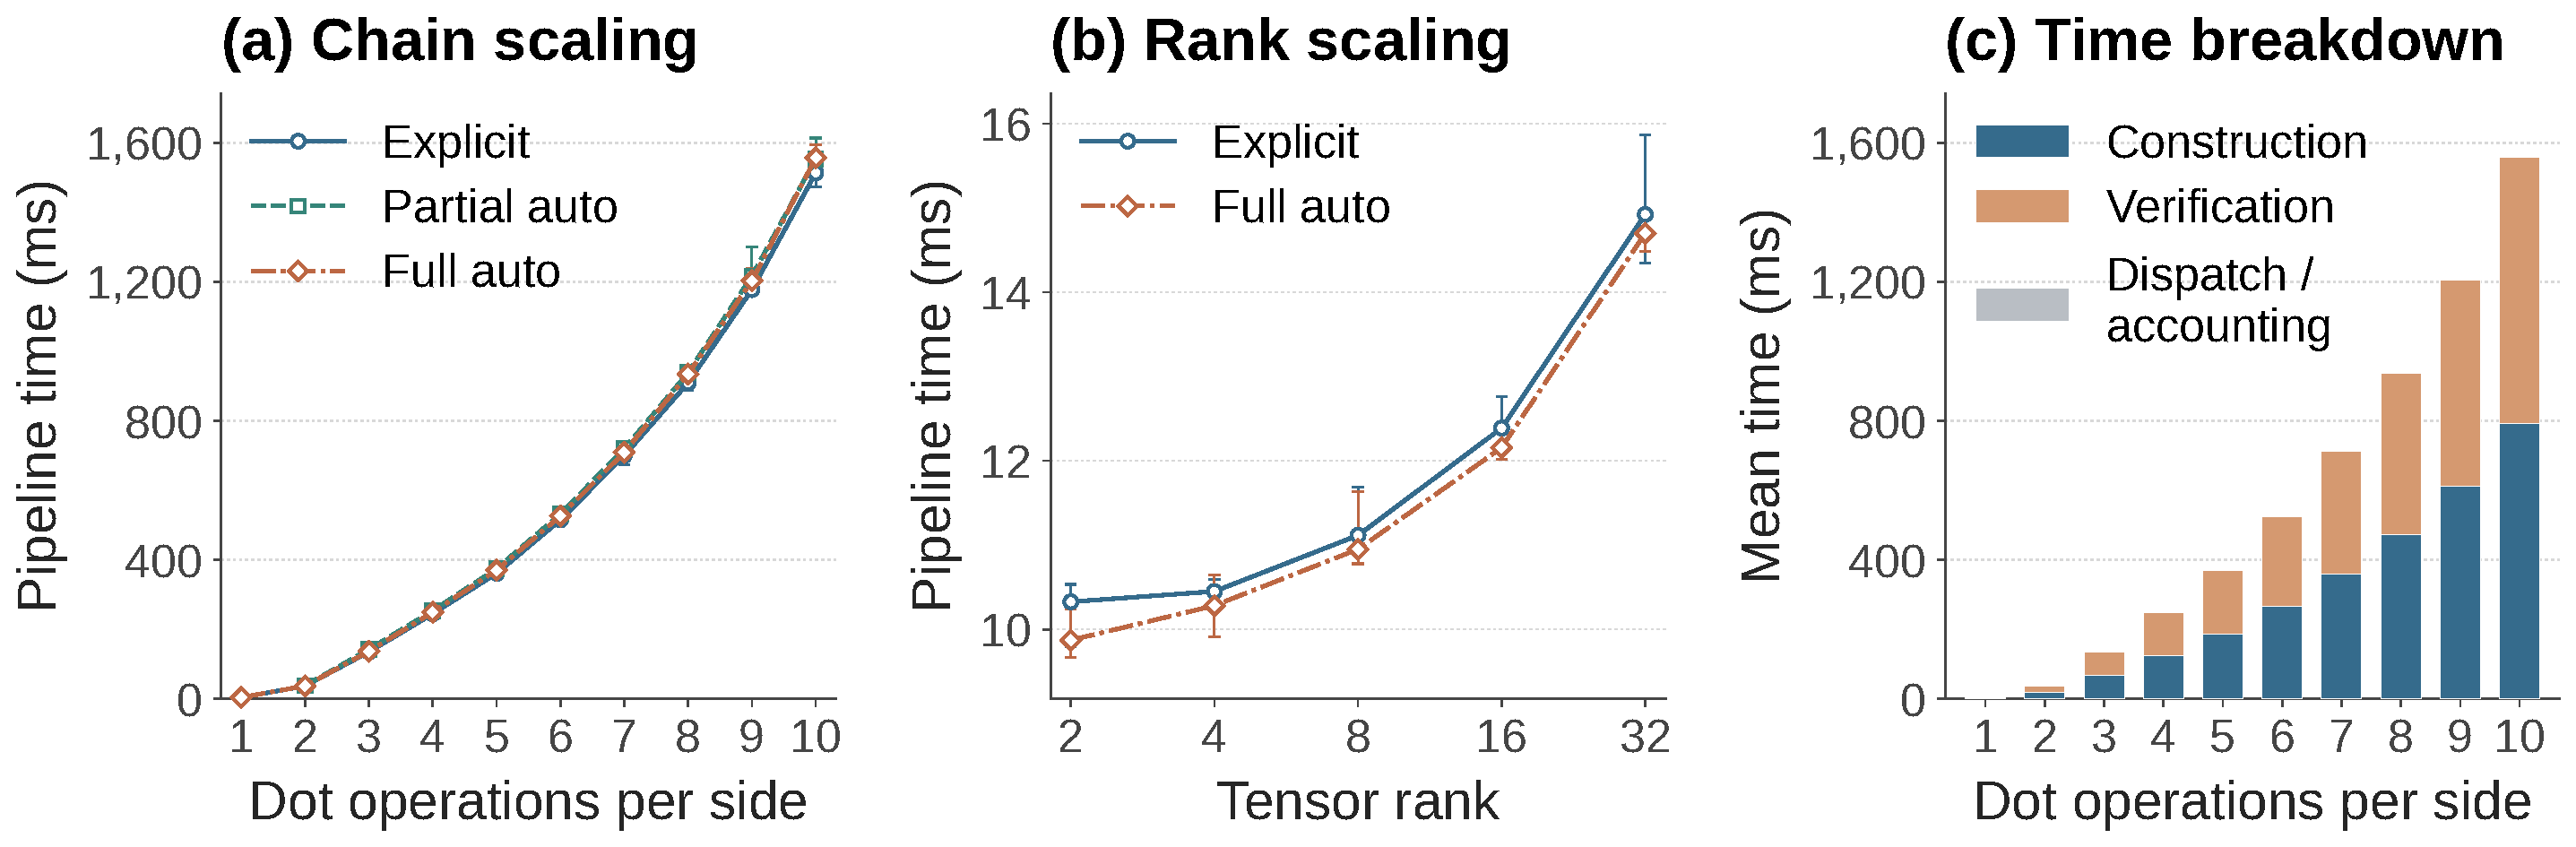
\includegraphics[width=\linewidth]{figures/scalability.pdf}
\caption{Construction and verification scaling: (a)~chains at rank three,
(b)~transpose ranks, and (c)~mean full-auto phase times.
Curves show medians and minimum--maximum whiskers.}
\label{fig:scalability}
\Description{Three panels show pipeline time increasing with the number of
dot operations, a modest increase with transpose rank, and stacked mean
times for construction, verification, and dispatch or accounting.}
\end{figure}

\begin{table}[!htbp]
\caption{Scalability results and their interpretation.}
\label{tab:scalability-results}
\centering
\small
\setlength{\tabcolsep}{4pt}
\begin{tabularx}{\linewidth}{@{}>{\raggedright\arraybackslash}p{0.17\linewidth}YY@{}}
\toprule
Aspect & Result & Interpretation\\\midrule
(a) Chain scaling
& Full-auto median time increases from 0.25~s at 4 dots to 1.56~s at 10 dots.
& Superlinear growth in this interval; no asymptotic bound is established.\\
\addlinespace
(b) Rank scaling
& Full-auto median time increases from 9.87~ms at rank 2 to 14.70~ms at rank 32.
& Rank has a modest effect for symbolic transpose composition.\\
\addlinespace
(c) Time breakdown
& At 10 dots, mean times are 0.793~s for construction and 0.765~s for verification.
& Both phases contribute substantially: approximately 51\% and 49\% of total time.\\
\addlinespace
Tested limits
& All 39 configurations succeed in every measured repetition within the deadline.
& Feasible over the tested range; no failure boundary is identified.\\\bottomrule
\end{tabularx}
\end{table}
\endgroup
\FloatBarrier

\paragraph{Interpretation and measurement limits.}
Figure~\ref{fig:scalability} and Table~\ref{tab:scalability-results} show
comparable total costs for explicit, partial-auto, and full-auto modes.
However, different solver paths mean that differences between their curves
do not directly isolate synthesis overhead.

The evaluation covers canonical contraction chains and symbolic transpose
composition. Larger graphs, other axis layouts, and other operator families
remain untested. Increasing chain length also increases expression depth,
so their effects are not separated. Measurements characterize metadata
reasoning rather than numerical tensor execution or end-to-end compilation.
Finally, five measured repetitions on one machine provide limited evidence
about runtime variability; the plotted minimum--maximum whiskers are not
confidence intervals.
\FloatBarrier

\end{document}
